\chapter{Búsqueda de SUSY con producción electrodébil en estados finales con fotones, bosones $Z$ y Higgs}\label{cap:analysis_EWK}
% \addcontentsline{toc}{chapter}{Búsqueda de SUSY con producción electrodébil}
\chaptermark{Búsqueda de SUSY con producción EWK con fotones, $Z$ y Higgs}

Las búsquedas de supersimetría están clasificadas por distintas características, en particular en la que se trabaja en esta tesis, está identificada con la producción fuerte de gluinos, y los resultados de la misma se muestran en los Capítulos anteriores. De forma análoga, es posible realizar una búsqueda con el mismo estado final, motivada por un modelo supersimétrico similar al anterior, pero dedicado a la producción electrodébil de partículas.

La metodología empleada para realizar dicha búsqueda consiste nuevamente en el modelado de muestras de señal y fondo, diseño de regiones sensibles a dicho modelo, y una posterior comparación entre las estimaciones de los fondos y los eventos observados. El presente Capítulo describe el diseño de una búsqueda con dichas características, su correspondiente validación y la sensibilidad esperada a una luminosidad de $139\,\ifb$. 


\section{Muestras de señal a partir de simulaciones de Monte Carlo}

El modelo que motiva a la presente búsqueda es una extensión al descripto en la Sección \ref{sec:signal_samples}. En el mismo se optimizaron los parámetros del modelo para obtener las masas y decaimientos deseados, en los cuales no estaba contemplado el decaimiento a bosones $Z$. La búsqueda electrodébil emplea una estrategia simplificada para generar las muestras de señal. En principio se fijan directamente las masas y los decaimientos de todas las partículas, sin centrarse en los parámetros de la teoría que llevan a tales valores. A su vez, la búsqueda se realiza de forma sensible a posibles decaimientos del \ninoone a fotones, bosones $Z$ y Higgs. La Figura \ref{fig:EWK_GGM_diagrams} muestra los posibles diagramas de decaimiento para la búsqueda electrodébil.


\begin{figure}
  \centering
  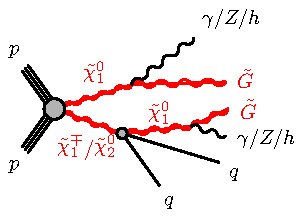
\includegraphics[width=0.45\textwidth]{images/analysis_EWK/N1N2C1-qqZhphGG-GGM.pdf}%
  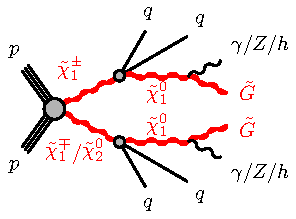
\includegraphics[width=0.45\textwidth]{images/analysis_EWK/C1C1N2-qqqqZhphGG-GGM.pdf}
  \caption{Diagramas de producción de gauginos con estado final de fotones, bosones $Z$, Higgs y gravitinos}
  \label{fig:EWK_GGM_diagrams}
\end{figure}


Se generan 12 puntos de señal en función de la masa del \ninoone, cuyos valores son: \magn{150}{GeV}, \magn{250}{GeV}, \magn{350}{GeV}, \magn{450}{GeV}, \magn{650}{GeV}, \magn{750}{GeV}, \magn{850}{GeV}, \magn{950}{GeV}, \magn{1050}{GeV}, \magn{1250}{GeV} y \magn{1450}{GeV}. Los decaimientos del mismos se fijaron a $33\%$ de igual forma para $\gamma + \gravino$, $Z + \gravino$ y $h + \gravino$. Los estados finales de cada evento están caracterizados por los posibles decaimientos de los dos \ninoone de la cadena de decaimiento, los cuales pueden ser $\gamma\gamma$, $\gamma Z$, $\gamma h$, $ZZ$, $Zh$ y $hh$ (omitiendo los \gravino por simplicidad). Al estar permitidos los tres decaimientos, es posible realizar un ponderado de los eventos, con el objetivo de estudiar diferentes combinaciones de fracciones de decaimiento. Es decir, aquellos decaimientos que no sean de interés, se los puede suprimir asignándole un peso nulo, permitiendo estudiar los otros dos restantes. Esto permite analizar diferentes modelos a partir de una misma muestra, y además calcular posibles límites de exclusión en función de las fracciones de decaimiento.
La metodología para asignar dichos pesos a los eventos va a depender, tanto de las fracciones de decaimiento que se deseen estudiar, como del tipo de partículas que se genera en el estado final. A nivel generador de las muestras, es posible saber cuáles partículas se generaron en los decaimientos de los \ninoone, y aplicarle el siguiente peso al evento:

% \begin{equation}
% \begin{split}
%   \textbf{w}(\text{BR}_{\gam}, \text{BR}_{Z}, \text{BR}_{h^{0}})  = &\ [w_{\gam\gam}, w_{\gam Z}, w_{\gam h^{0}}, w_{ZZ}, w_{Zh^{0}}, w_{h^{0}h^{0}}] \\
%      = &\ \left(\frac{1}{3}\right)^{-2} \cdot [\text{BR}_{\gam}^{2}, \text{BR}_{\gam}\cdot\text{BR}_{Z}, \text{BR}_{\gam}\cdot\text{BR}_{h^{0}}, \text{BR}_{Z}^{2}, \text{BR}_{Z}\cdot\text{BR}_{h^{0}}, \text{BR}_{h^{0}}^{2}] \\
% \end{split}
% \end{equation}


\begin{equation}
  w(\text{BR}_{\gamma}, \text{BR}_{Z}, \text{BR}_{h^{0}})=\left(\frac{1}{3}\right)^{-2}\cdot\begin{cases}
    \text{BR}_{\gamma}^{2} & \text{si el par es } \gamma\gamma \\
    \text{BR}_{\gamma}\cdot\text{BR}_{Z} & \text{si el par es } \gamma Z \\
    \text{BR}_{\gamma}\cdot\text{BR}_{h^{0}} & \text{si el par es } \gamma h \\
    \text{BR}_{Z}^{2} & \text{si el par es } ZZ \\
    \text{BR}_{Z}\cdot\text{BR}_{h^{0}} & \text{si el par es } Zh \\
    \text{BR}_{h^{0}}^{2} & \text{si el par es } hh \\
  \end{cases}
\end{equation}

\noindent
donde $\text{BR}_{X}$ es la fracción de decaimiento del proceso $\ninoone \to \gravino X$ que se desea estudiar.
El peso está normalizado de tal forma que la suma de todas las fracciones de decaimiento de la unidad. En particular, y a modo de estudio preliminar, la búsqueda se centra en dos modelos: el modelo equivalente al estudiado en la producción fuerte, donde el \ninoone decae $50\%$ a $\gamma + \gravino$ y $50\%$ a $\gamma + h$, denominado modelo <<ph+h>> donde $w(0.5, 0, 0.5)$. Y por otro lado, el modelo donde el \ninoone decae $50\%$ a $\gamma + \gravino$ y $50\%$ a $\gamma + Z$, denominado modelo <<ph+Z>> donde $w(0.5, 0.5, 0)$.

Las masas del \ninotwo y \chinopm se eligen levemente degeneradas, e iguales a la del \ninoone más \magn{10}{GeV} y \magn{11}{GeV} respectivamente. 
% \solved{justificar esto?} fue una primera referencia para una posible extension
Sus decaimientos se fijan en $100\%$ al \ninoone a través de un $Z$ o $W$ virtual, con sus respectivos decaimientos del SM. Todas las demás partículas SUSY se desacoplan con una masa de \magn{4500}{GeV}. A partir de ellos, se consideran todos los posibles canales de producción electrodébil, los cuales son: $\ninoone \ninotwo$, $\ninoone \chinoonepm$, $\ninotwo \chinoonepm$ y $\chinoonep \chinoonem$. La sección eficaz de producción de cada uno se calcula utilizando \texttt{RESUMMINO-3.0.0} \cite{Beenakker:1999xh,Debove:2010kf,Fuks:2012qx,Fuks:2013vua,Fiaschi:2018hgm} con una precisión de NLO+NLL, utilizando la familia de PDFs \texttt{CTEQ6.6} y \texttt{MSTW2008}, siguiendo las recomendaciones de \texttt{PDF4LHC} \cite{Butterworth:2015oua}. La Figura \ref{fig:SUSY_EWK_xs} muestra las secciones eficaces de cada proceso junto con la total.

\begin{figure}
  \centering
  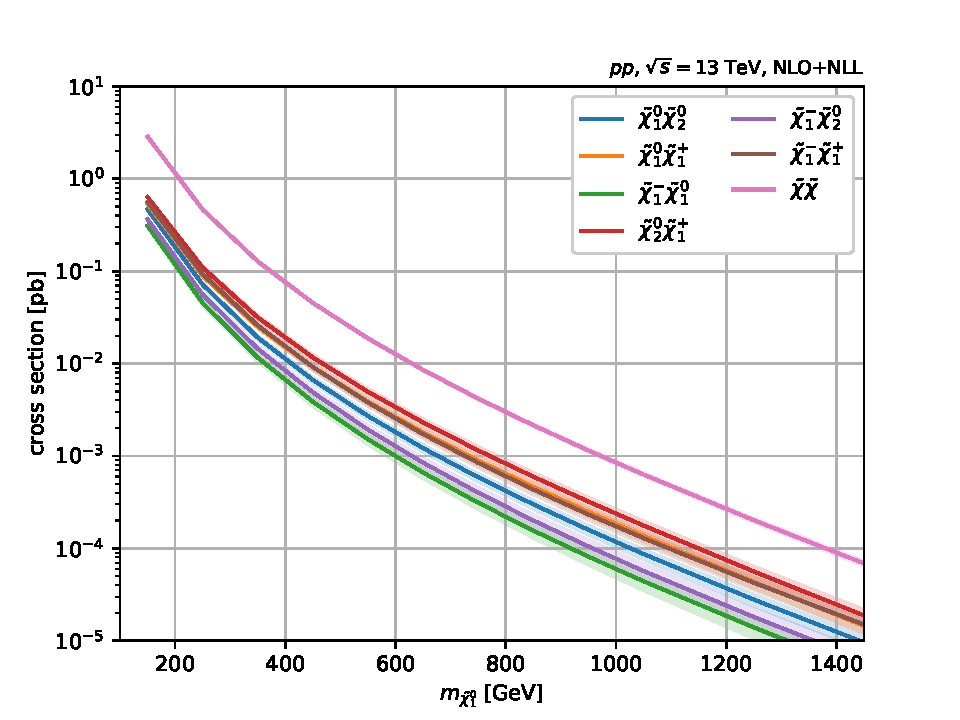
\includegraphics[width=0.7\textwidth]{images/analysis_EWK/SUSY_EWK_xsecs_m.pdf}
  \caption{Sección eficaz de la producción de gauginos en función de la masa de \ninoone. En rosa la sección eficaz total considerando todos los procesos.}
  \label{fig:SUSY_EWK_xs}
\end{figure}



\section{Fondos del Modelo Estándar}

Tantos las simulaciones de fondos del SM, como las técnicas para modelar fondos a partir de datos descriptas en la Sección \ref{sec:sm_backgrounds}, se emplean de forma equivalente para esta búsqueda. Adicionalmente, se incluye el fondo de producción de tops y bosones de Higgs decayendo a fotones \cite{tesis_jose}, listadas en la Tabla \ref{tab:higgs_bkg}. Esto está motivado por el valor del factor de normalización obtenido para la región de control CRT, que al ser superior a la unidad, puede ser un indicio de que algún proceso con el mismo estado final no está siendo considerado.

\begin{table}[h!]
  \centering
  \caption{Muestras de fondos de MC con producción de tops y bosones de Higgs decayendo a fotones, utilizadas en el análisis con producción electrodébil, donde se especifica su generador, sección eficaz, $k$-factor y eficiencia de filtro.}
  \label{tab:higgs_bkg}
  \resizebox{\textwidth}{!}{
  \begin{tabular}{llrrr}

     \hline
      \hline
    Proceso & Generador & Sección Eficaz [pb] & $k$-factor & Eficiencia de filtro \\

    \hline
     \hline

    $\ttbar h(\to \gamma\gamma)$  & \texttt{Powheg\_aMC@NLO}/\texttt{Pythia8} & 0.52493  & 1.0 & 1.0  \\
    $\ttbar h(\to Z\gamma)$  & \texttt{Powheg\_aMC@NLO}/\texttt{Pythia8} & 0.52492  & 1.0 & 1.0  \\

    \hline
     \hline
  \end{tabular}
  }
\end{table}



\section{Selección de eventos y objetos para el análisis}

Para la presente búsqueda se emplea el conjunto de datos con centro de masa de \magn{13}{TeV}, y una luminosidad integrada de \magn{139}{\ifb} tomados durante el Run 2. Los datos son seleccionados con el trigger \texttt{HLT\_g140\_loose}, y empleando la derivación \texttt{SUSY1} tanto para los datos como para las simulaciones. La selección de objetos es similar a la descripta en la Sección \ref{sec:selection}, con leves modificaciones en los leptones y jets. Dentro de la colaboración existen grupos dedicados a combinar los resultados obtenidos para distintos análisis de SUSY. Para ello, los análisis combinados deben tener selecciones ortogonales, por lo que se establece una selección particular de leptones para lograr dicho objetivo. La presente búsqueda, en base a una posible combinación con otros análisis, selecciona electrones baseline con un $\pt>4.5\ \gev$ y los signal con un $\pt>10 \ \gev$, mientras que los muones baseline se seleccionan con un $\pt>3\ \gev$ y los signal con un $\pt>10\ \gev$. A su vez en todas las regiones del análisis se solicita que el número de leptones baseline sea igual al número de leptones signal. Los jets empleados en la selección de eventos son \texttt{PFlow} jets con un $\pt>20\ \gev$. El algoritmo para identificar $b$-jets es el \texttt{DL1r}, con un $77\%$ de eficiencia.



\section{Definición de las regiones del análisis}

La definición de las regiones de señal se realiza siguiendo metodología de optimización similar a la descripta en la Sección \ref{sec:sig_selection}.
Si bien el estado final de esta búsqueda coincide con la búsqueda anterior, la cinemática de los mismos tiene algunos aspectos distintos. Dada la baja masa de los gauginos producidos en la colisión, con respecto a la producción de gluinos, se espera que los productos generados en el decaimiento sean menos energéticos. Con el mismo criterio, el número de jets reconstruidos de la cadena de decaimiento se espera que sea menor.

Se diseñan cuatro regiones de señal dedicadas a cubrir todo el espectro de masas de \ninoone de las muestras de señal. Las regiones se definen con cortes comunes para todas, salvo por un corte inclusivo en \met. Estos cortes consisten en al menos un fotón con $\pt>145\ \gev$, un veto de leptones, al menos un jet, y separaciones angulares de \dphijetmet y \dphigammet mayores a $0.4$. A su vez, se incluyen cortes en dos variables adicionales para incrementar la separación de señal y fondo. La primera definida como:

\begin{equation}
  \frac{\met}{\meff} = \frac{\met}{\HT + \met}
\end{equation}

La misma se entiende como la fracción de \met presente con respecto a la energía total presente en el evento, que para una señal de SUSY con gran actividad de partículas no interactuantes es esperable que sea mayor a $0.5$.
% \solved{en realidad todavía no entendemos esta variable...} % ponele que si
La segunda variable empleada es la Significancia de \met ($\mathcal{S}$), con una reconstrucción denominada \textit{object-based} descripta en la Referencia \cite{ATLAS-CONF-2018-038}. La misma sirve para discriminar eventos con \met proveniente de partículas poco interactuantes, de aquella producto de la reconstrucción ineficiente de las partículas (instrumental), ya que valores altos de $\mathcal{S}$ son un indicio del primer caso. Finalmente, y solo en el caso de eventos con dos fotones, se aplica un corte en la masa invariante de los mismos, excluyendo el rango de valores centrados en la masa del Higgs. Esto se hace con el objetivo de ser ortogonales al análisis con estado final similar, que selecciona dos fotones provenientes del decaimiento del bosón de Higgs. La selección empleada para las distintas regiones de señal se muestra en la Tabla \ref{tab:sr_ewk}.



\begin{table} 
\centering
  \caption{Regiones de señal de descubrimiento, empleadas para el análisis de búsqueda de SUSY con producción electrodébil.}
  % \resizebox{\linewidth}{!}{
    \begin{tabular}{ l | c | c | c | c }
    \hline
    \hline
      & SRd\_200 & SRd\_300 & SRd\_400 & SRd\_500 \\
    \hline
    \hline
    % Trigger & \multicolumn{4}{c}{g140\_loose} \\
    % \hline
    \nph & \multicolumn{4}{c}{$\ge1$} \\
    % \hline
    \nlep & \multicolumn{4}{c}{$0$} \\
    % \hline
    \njet & \multicolumn{4}{c}{$\ge1$} \\
    % \hline
    \ptph [GeV] & \multicolumn{4}{c}{$>145$} \\
    % \hline
    $\met/\meff$ & \multicolumn{4}{c}{$>0.5$} \\
    % \hline
    $\mathcal{S}$ & \multicolumn{4}{c}{$>21$} \\
    % \hline
    \dphijetmet & \multicolumn{4}{c}{$>0.4$} \\
    % \hline
    \dphigammet & \multicolumn{4}{c}{$>0.4$} \\
    % \hline
    \myy [GeV]& \multicolumn{4}{c}{$<120,\ >130$} \\
    % \hline
    \cline{2-5}
    \met [GeV] & $>200$ & $>300$ & $>400$ & $>500$ \\
    \hline
    \hline
      \end{tabular}
  % }
  \label{tab:sr_ewk}
\end{table}


% \solved{mencionar SRs para exclusion?} done

Las regiones de señal anteriormente mencionadas, están diseñadas para obtener la mejor significancia esperada, lo que no implica que en el caso hipotético de no observar algún descubrimiento, los límites esperados que se impongan con las mismas sean los más óptimos. 
En base a eso, se diseña un conjunto de regiones señal destinadas exclusivamente a imponer límites de exclusión. Para poder distinguirlas, se denomina a las primeras como regiones de señal para descubrimiento (SRd\_XXX), y a las segundas para exclusión (SRe\_XXX). Las regiones para exclusión se obtienen en base a las de descubrimiento, modificando sus cortes para obtener la combinación que permita tener los límites esperados más altos. Para tener una estimación preliminar de dichos límites, se emplea la aproximación asintótica enunciada en la Sección \ref{sec:aprox_test}, y se omiten los sistemáticos para simplificar los cálculos. Se encuentra que para obtener mejores limites, los cortes en \met no deben ser inclusivos (sino ortogonales), y que además se debe omitir el corte en $\met/\meff$. La definición de las regiones de señal para exclusión se muestran en la Tabla \ref{tab:sr_ewk_excl}.

\begin{table} 
\centering
  \caption{Regiones de señal para exclusión, empleadas para el análisis de búsqueda de SUSY con producción electrodébil.}
  % \resizebox{\linewidth}{!}{
  \begin{tabular}{ l | c | c | c | c }
  \hline
  \hline
    & SRe\_200 & SRe\_300 & SRe\_400 & SRe\_500 \\
  \hline
  \hline
  Trigger & \multicolumn{4}{c}{g140\_loose} \\
  % \hline
  \nph & \multicolumn{4}{c}{$\ge1$} \\
  % \hline
  \nlep & \multicolumn{4}{c}{$0$} \\
  % \hline
  \njet & \multicolumn{4}{c}{$\ge1$} \\
  % \hline
  \ptph [GeV] & \multicolumn{4}{c}{$>145$} \\
  % \hline
  $\mathcal{S}$ & \multicolumn{4}{c}{$>21$} \\
  % \hline
  \dphijetmet & \multicolumn{4}{c}{$>0.4$} \\
  % \hline
  \dphigammet & \multicolumn{4}{c}{$>0.4$} \\
  % \hline
  \cline{2-5}
  \met [GeV] & $[200-300]$ & $[300-400]$ & $[400-500]$ & $>500$ \\
  \hline
  \hline
    \end{tabular}
      % }
      \label{tab:sr_ewk_excl}
    \end{table}


Los fondos del SM con mayor impacto en el análisis son \wph, \ttbarph, $\ttbar h$ y \znunuph, para las cuales se diseñan regiones de control dedicadas. El fondo \phj no se considera importante, debido a la presente selección en los objetos del estado final buscado, y por ende no tiene su respectiva región de control. Todas las regiones de control emplean selecciones similares a las descriptas en la Sección \ref{sec:cr_vr_sel} para favorecer cada fondo, pero adaptadas a las actuales SRs. En todas se omite el corte en $\met/\meff$ y $\mathcal{S}$, debido a la elevada reducción de fondo que producen.


Los fondos \ttbarph y $\ttbar h$, son normalizados simultáneamente en una región de control (CRT) que selecciona al menos un leptón y dos $b$-jets. Para el fondo de \wph se diseña una región de control (CRW) que selecciona un leptón con un veto a los $b$-jets, junto con un corte en la masa transversa de \met y el leptón\footnote{$\mtlep = \sqrt{2p_{\text{T}}^{\text{leptón}}\met[1-\cos(\phi^{\text{miss}}-\phi^{\text{leptón}})]}$}, para incrementar la pureza del fondo. Dado que el fondo de \znunuph presenta un estado final similar al de la señal, resulta prácticamente imposible diseñar una región de control para ese fondo que no tenga contaminación de señal. Para ello, se emplea un método alternativo, en donde se diseñan regiones de control para los procesos \zeeph y \zmumuph (CRZ\_el y CRZ\_mu), y se asume que las correcciones que necesita la simulación son equivalentes para la simulación de \znunuph, por lo que se aplica el mismo factor de normalización a los tres fondos simultáneamente. Como los fondos \zeeph y \zmumuph tienen \met despreciable, se construye una una energía transversa alternativa pero omitiendo del cálculo a los leptones. De esta forma se obtiene una \met alineada con los leptones del evento, a la cual se le aplica un corte para ser lo más similar posible a las SRs. A su vez, los cortes empleados para \dphijetmet y \dphigammet se obtienen en base a este cálculo de \met. En la Figura \ref{fig:met_inv} se puede observar una comparación entre \met de \znunuph y la reconstruida en las simulaciones de \zeeph y \zmumuph, en la que se demuestra un buen acuerdo entre las distintas estimaciones de \met. La definición de las regiones de control empleadas para el presente análisis se muestran en la Tabla \ref{tab:cr_ewk}.

\begin{figure}
  \centering
  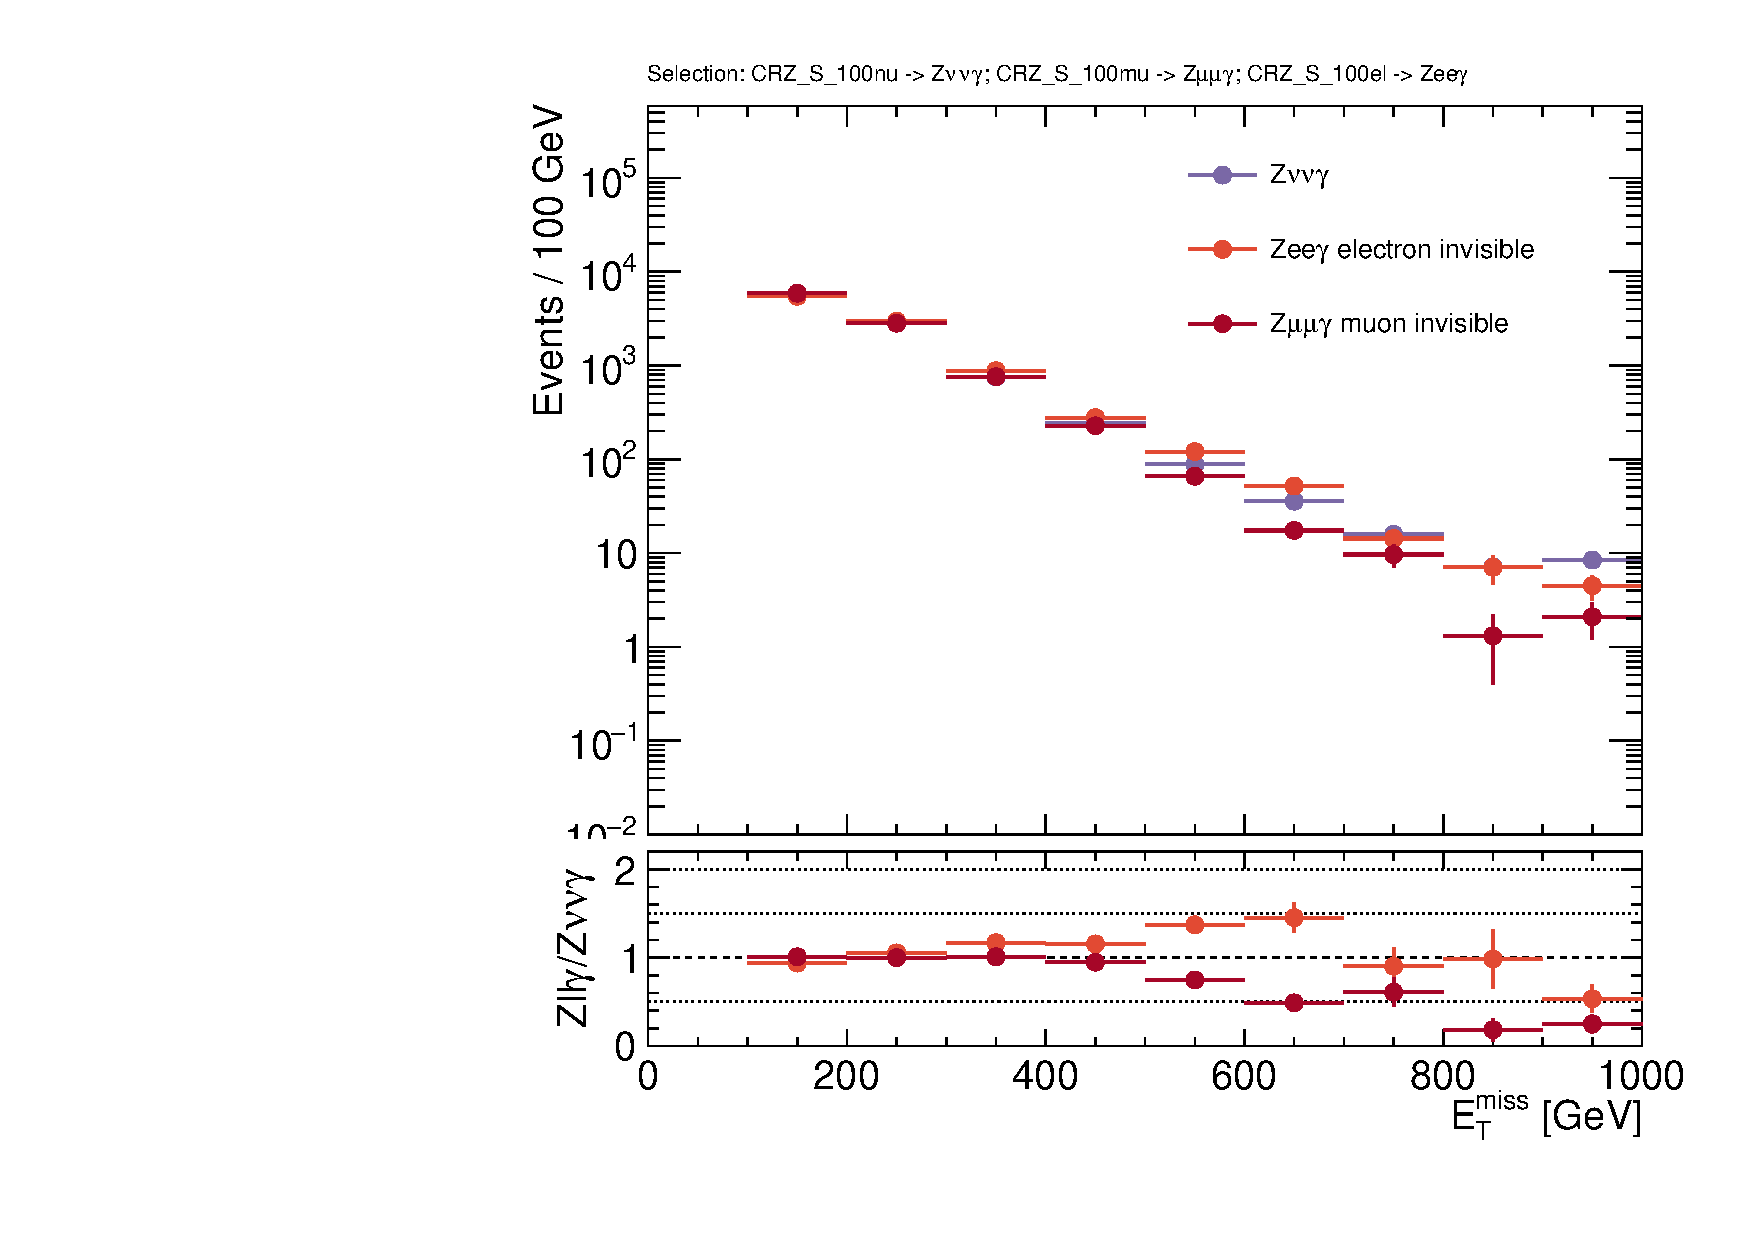
\includegraphics[width=0.24\textwidth]{images/analysis_EWK/ZnunugCutS_100_vs_ZllgCutS_100_v192_0_met_et.pdf}
  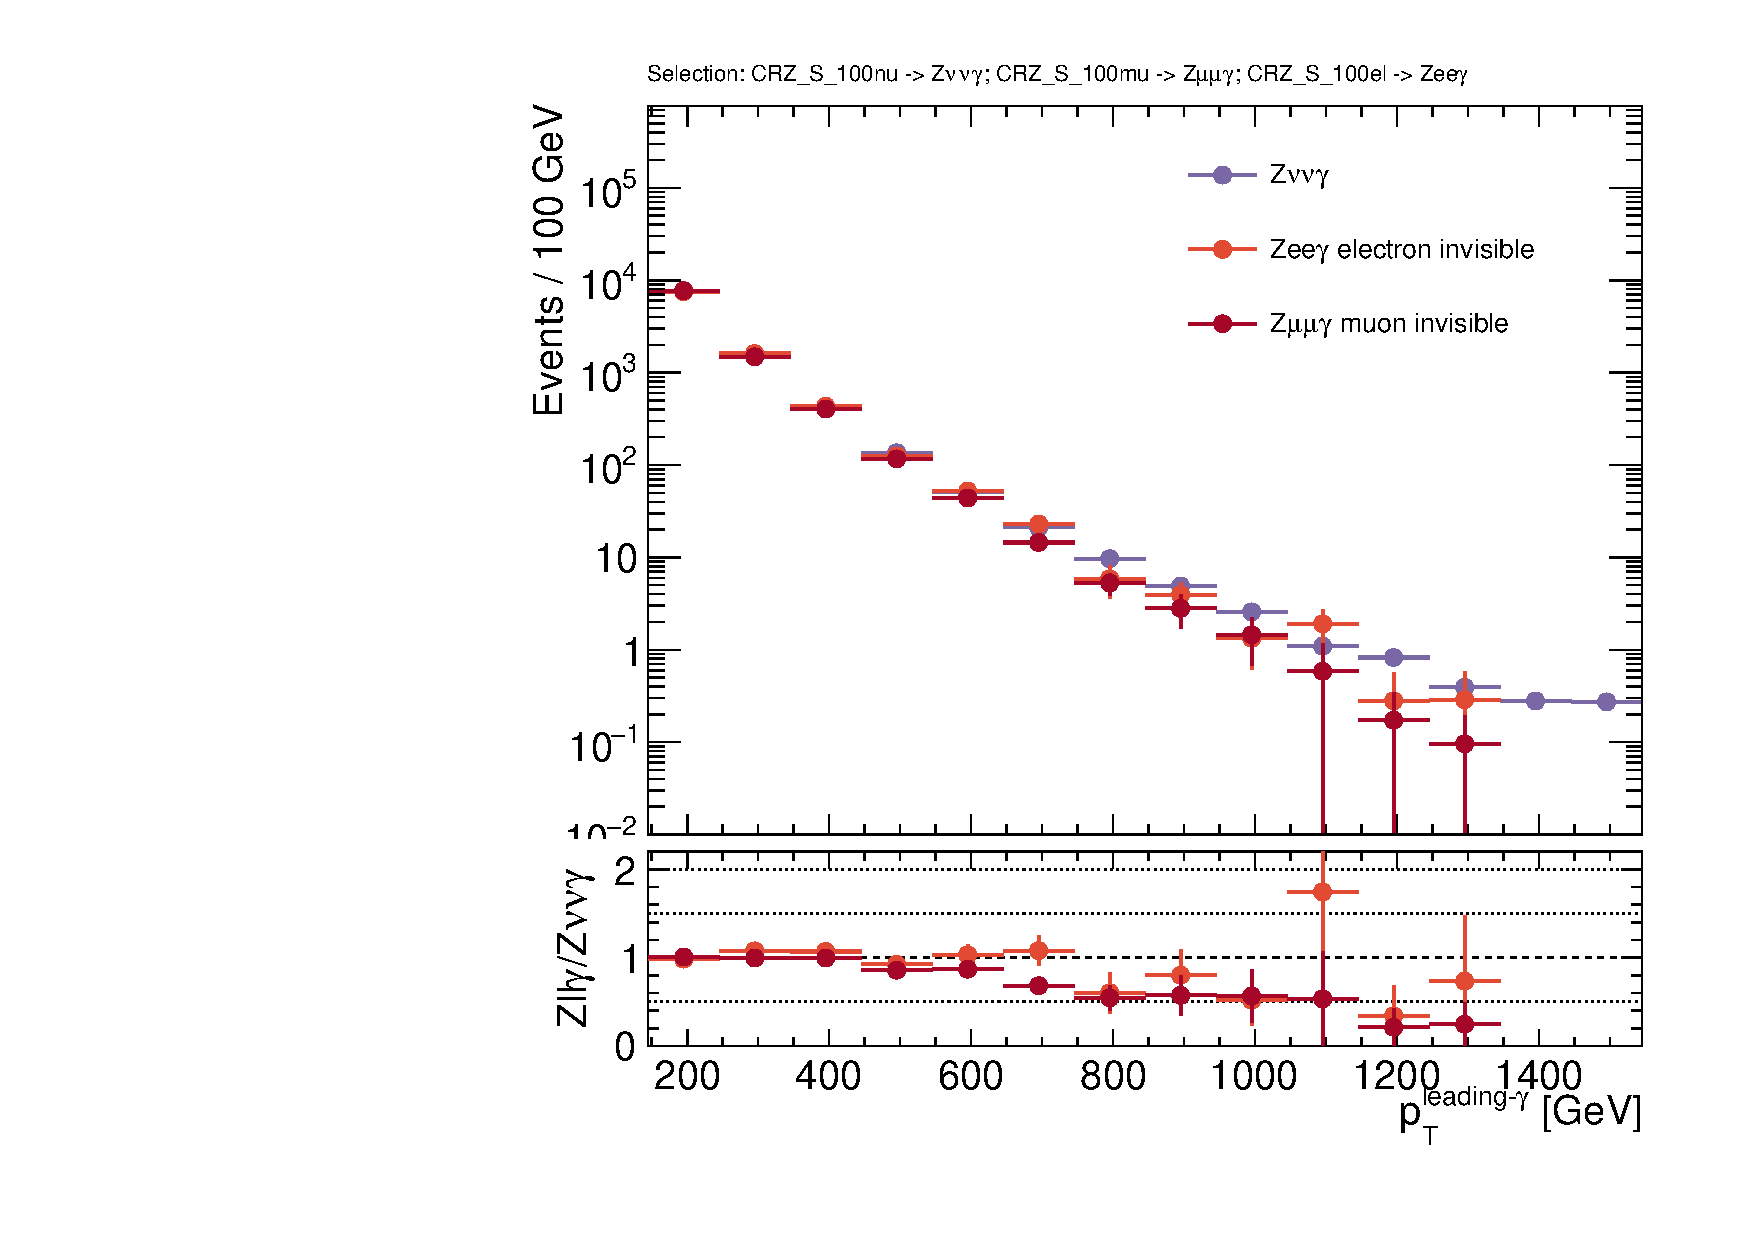
\includegraphics[width=0.24\textwidth]{images/analysis_EWK/ZnunugCutS_100_vs_ZllgCutS_100_v192_0_ph_pt0.pdf}
  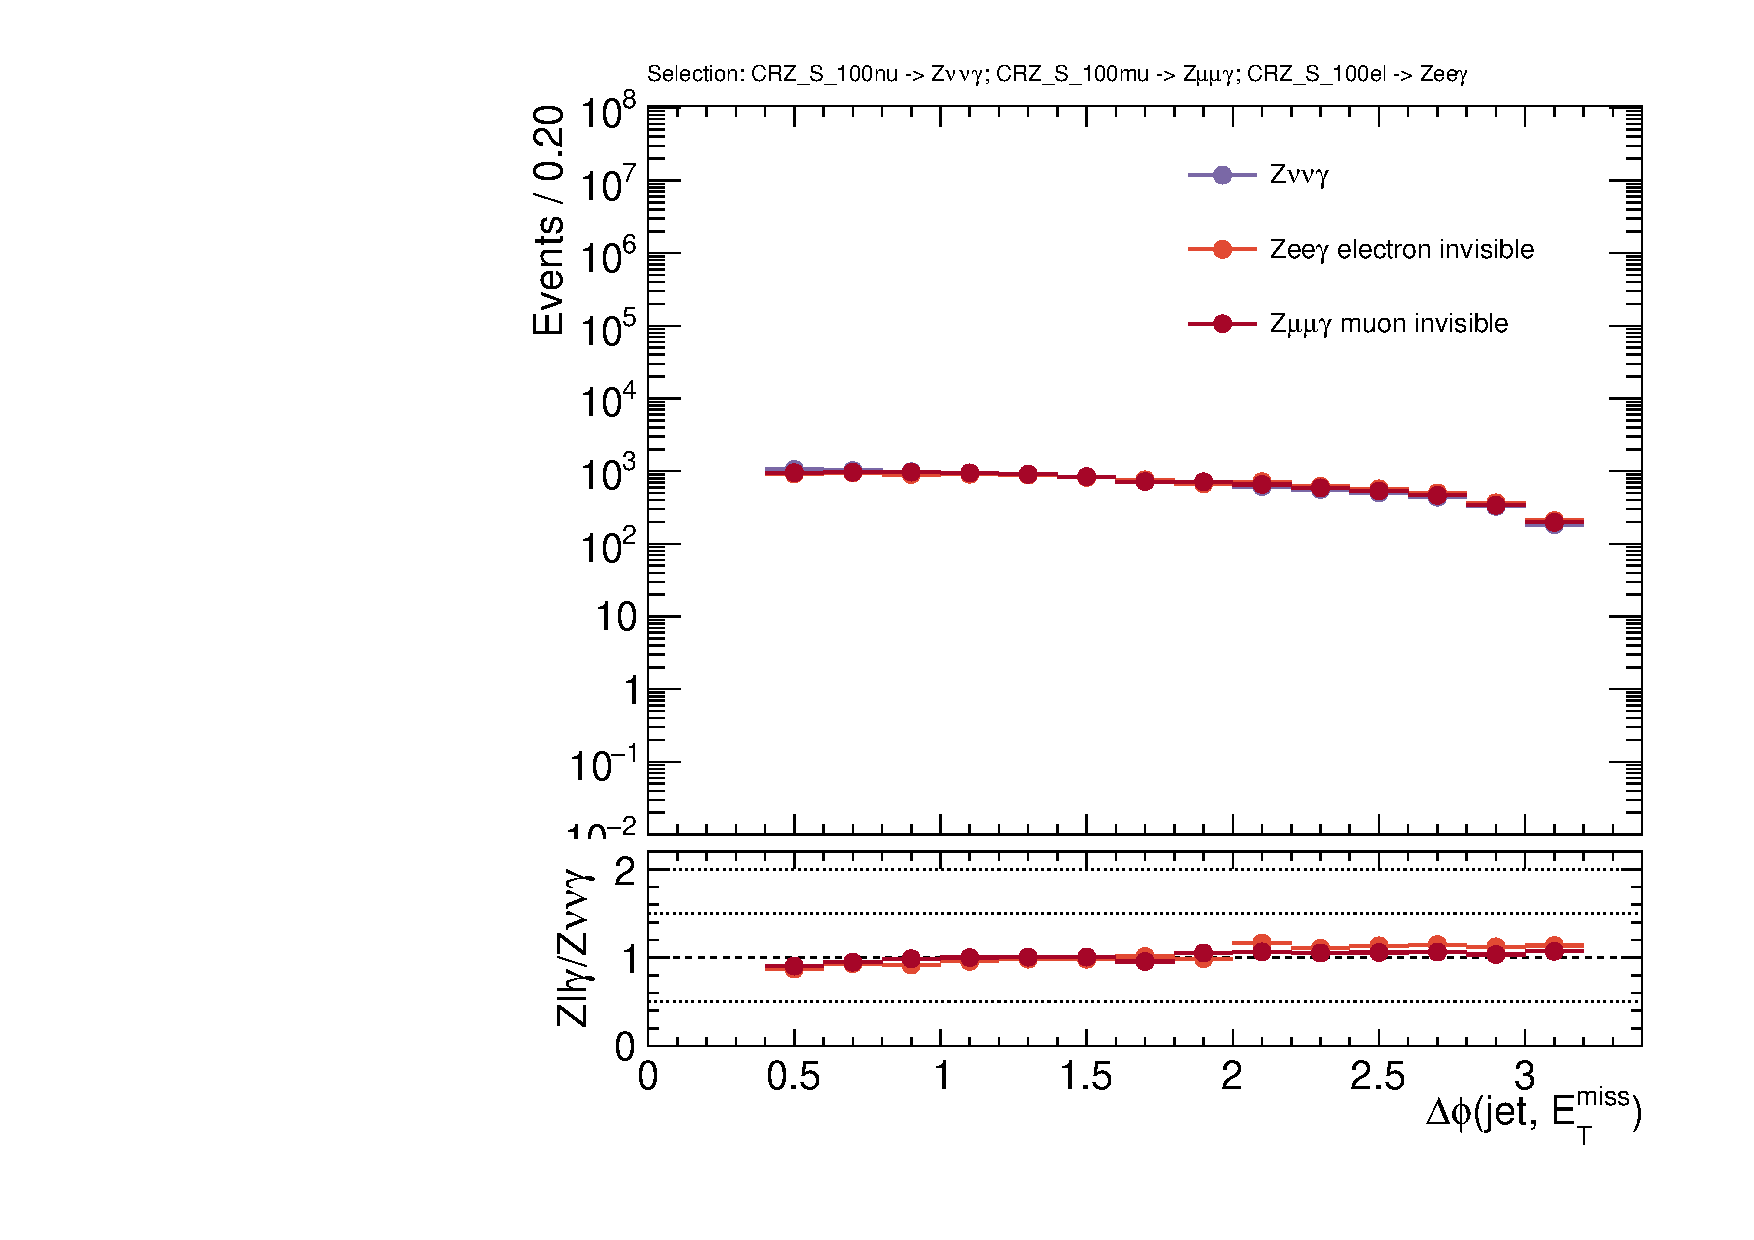
\includegraphics[width=0.24\textwidth]{images/analysis_EWK/ZnunugCutS_100_vs_ZllgCutS_100_v192_0_dphi_jetmet.pdf}
  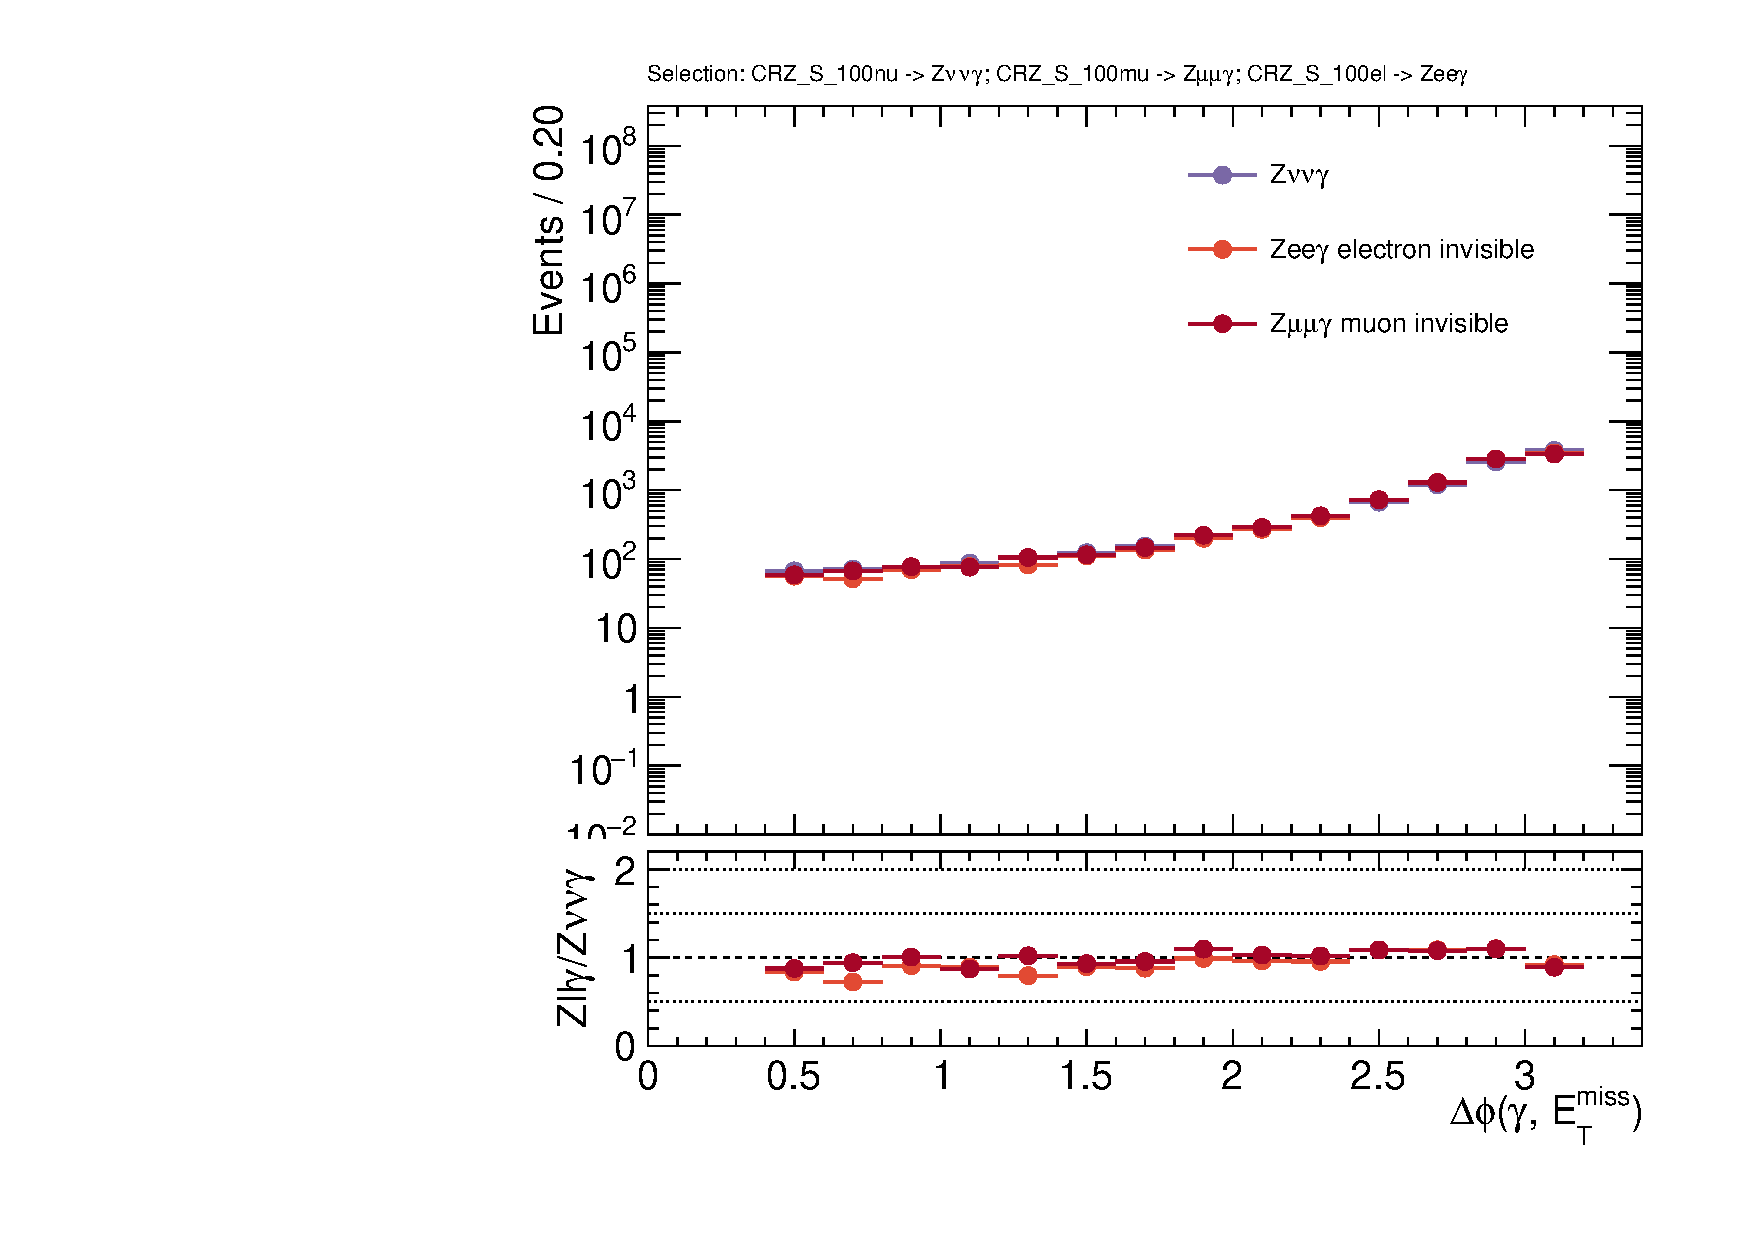
\includegraphics[width=0.24\textwidth]{images/analysis_EWK/ZnunugCutS_100_vs_ZllgCutS_100_v192_0_dphi_gammet.pdf}
  \caption{Comparación de \met en el fondo de \znunuph y la reconstruida para los fondos de \zeeph y \zmumuph.}
  \label{fig:met_inv}
\end{figure}

\begin{table}
\centering
    \caption{Definición de las regiones de control para el análisis con producción electrodébil. El asterisco en las variables que emplean \met representa que el valor de dicha variable es estimado removiendo los leptones del cálculo.}
  % \resizebox{\linewidth}{!}{
    \begin{tabular}{ l | c | c | c | c }
    \hline
    \hline
      & CRW & CRT & CRZ\_el & CRZ\_mu \\
    \hline
    \hline
    % Trigger & \multicolumn{4}{c}{g140\_loose} \\
    % \hline
    \nph & \multicolumn{4}{c}{$\ge1$} \\
    % \hline
    \ptph [GeV] & \multicolumn{4}{c}{$>145$} \\
    % \hline
    \njet & \multicolumn{4}{c}{$\ge1$} \\
    % \hline
    \cline{2-5}
    \nbjet & 0 & $\ge 2$ & - & - \\
    % \hline
    \nlep & \cellcolor{lightgreen} $1$ & \cellcolor{lightgreen} $\ge1$ & \cellcolor{lightgreen} $2$ (el) & \cellcolor{lightgreen} $2$ (mu) \\
    % \hline
    \dphijetmet & $>0.4$ & $>0.4$ & $>0.4$ (*) & $>0.4$ (*)\\
    % \hline
    \dphigammet & $>0.4$ & $>0.4$ & $>0.4$ (*) & $>0.4$ (*)\\
    % \hline
    \met [GeV] & $>200$ & $>150$ & $<50$ & $<50$ \\
    % \hline
    \met (*) [GeV] & - & - & $>100$ & $>100$ \\
    % \hline
    \mtlep [GeV] & $<100$ & - & - & - \\
    \hline
    \hline
    % $m_{ll}$ [GeV] & - & - & $[80-100]$ & $[80-100]$ \\
    % \hline
    \end{tabular}
    \label{tab:cr_ewk}
  % }
\end{table}



Finalmente se incluye un diseño preliminar para regiones de validación. Las mismas se diseñan para validar la extrapolación de los distintos fondos normalizados en las control regiones, a las regiones de señal. Se diseñan cinco regiones de señal, cuatro asociadas a las regiones de control (VRW, VRT, VRZee y VRZmm) y una adicional para el fondo de electrones reconstruidos erróneamente como fotones (VRE). Las regiones basadas en las CRs incluyen ahora el corte en $\met/\meff$ y $\mathcal{S}$ para acercarse cinemáticamente a las SRs, y son ortogonales a estas últimas debido a la selección de leptones. La VRE se construye invirtiendo el corte en \dphigammet, favoreciendo al fondo de \textit{efakes}, y adicionalmente siendo ortogonal a las regiones de señal. En la Tabla \ref{tab:vr_ewk} se muestran las definiciones de las regiones de validación.



\begin{table}
\centering
    \caption{Definición de las regiones de validación para el análisis con producción electrodébil. El asterisco en las variables que emplean \met representa que el valor de dicha variable es estimado removiendo los leptones del cálculo.}
  % \resizebox{\linewidth}{!}{
      \begin{tabular}{ l | c | c | c | c | c }
      \hline
      \hline
        & VRW & VRT & VRZee & VRZmm & VRE \\
      \hline
      \hline
      Trigger & \multicolumn{5}{c}{g140\_loose} \\
      % \hline
      \nph & \multicolumn{5}{c}{$\ge1$} \\
      % \hline
      \ptph [GeV] & \multicolumn{5}{c}{$>145$} \\
      % \hline
      \njet & \multicolumn{5}{c}{$\ge1$} \\
      \cline{2-6}
      % \hline
      \nlep & \cellcolor{lightgreen} $1$ & \cellcolor{lightgreen} $\ge1$ & \cellcolor{lightgreen} $2$ (el) & \cellcolor{lightgreen} $2$ (mu) & - \\
      % \hline
      \dphijetmet & $>0.4$ & $>0.4$ & $>0.4$ (*) & $>0.4$ (*) & $>0.4$\\
      % \hline
      \dphigammet & $>0.4$ & $>0.4$ & $>0.4$ (*) & $>0.4$ (*) & \cellcolor{lightgreen} $<0.4$ \\
      % \hline
      \met [GeV] & $>200$ & $>200$ & $<50$ & $<50$ & $>200$ \\
      % \hline
      $\met/\meff$ & $>0.25$ & $>0.2$ & $>0.25$ & $>0.25$ & $>0.25$ \\
      % \hline
      $\mathcal{S}$ & $>10$ & $>8$ & $>10$  & $>10$  & $>10$  \\
      % \hline
      \met (*) [GeV] & - & - & $>200$ & $>200$ & - \\
      \hline
      \hline
      \end{tabular}
      \label{tab:vr_ewk}
  % }
\end{table}

\section{Resultados preliminares}

% \solved{Arreglar sistematicos en las tablas} % Done


En la Tabla \ref{tab:bkg_only_fit_ewk} se muestran los resultados preliminares del ajuste de solo fondo, empleando las cuatro regiones de control. En las mismas se muestra el aporte de cada fondo antes y después del ajuste, junto con la pureza del fondo y el factor de normalización. Los fondos \ttbarph y $\ttbar h$ se ajustan con el mismo factor de normalización en la CRT, mientras que los fondos de \znunuph, \zeeph y \zmumuph lo hacen con su respectivo factor en las CRZ\_el y CRZ\_mu. De forma preliminar se emplea un sistemático \textit{dummy} del $25\%$ para todos los fondos en todas las regiones, emulando el aporte de los sistemáticos teóricos y del detector, observado en el análisis descripto en el Capítulo \ref{cap:analysis}. En general se obtuvieron factores de normalización cercanos a la unidad, lo que evidencia un correcto modelado por parte de las simulaciones. En las Figuras \ref{fig:crw_crt_dist_ewk} y \ref{fig:crz_el_mu_dist_ewk} se puede observar el buen acuerdo entre las simulaciones y los datos luego del ajuste.

\begin{table}
  \centering
  \caption{Resultados preliminares del ajuste de solo fondo en las diferentes regiones de control para el análisis de producción electrodébil. Se muestran los resultados antes y después del ajuste, la pureza del fondo y los factores de normalización.}
  \resizebox{\textwidth}{!}{\begin{tabular}{lrrrr}
\hline
Control Regions & CRW & CRT & CRZ\_mu & CRZ\_el \\
\hline
Observed events & 1378 & 471 & 1032 & 776 \\
\hline
Expected SM events & $1377.00 \pm 36.96$ & $470.93 \pm 21.64$ & $1043.42 \pm 24.48$ & $764.42 \pm 17.87$ \\
\hline
$t\bar{t}\gamma$ & $25.50 \pm 3.74$ & $203.86 \pm 29.90$ & $8.33 \pm 1.22$ & $5.91 \pm 0.87$ \\
$t\bar{t}h(\gamma\gamma/Z\gamma)$ & $17.58 \pm 3.17$ & $154.64 \pm 27.85$ & $6.03 \pm 1.09$ & $5.12 \pm 0.92$ \\
$W\gamma$ & $1168.05 \pm 43.98$ & $16.59 \pm 0.62$ & $0.49 \pm 0.02$ & $0.88 \pm 0.03$ \\
$Z(\nu\nu)\gamma$ & $0.76 \pm 0.21$ & $0.02 \pm 0.01$ & $0.00 \pm 0.00$ & $0.00 \pm 0.00$ \\
$\gamma + \text{jets}$ & $2.30 \pm 0.46$ & $1.68 \pm 0.33$ & $1.71 \pm 0.34$ & $0.00 \pm 0.00$ \\
$\gamma\gamma/W\gamma\gamma/Z\gamma\gamma$ & $36.51 \pm 7.26$ & $0.55 \pm 0.11$ & $36.82 \pm 7.32$ & $24.20 \pm 4.81$ \\
$Z(ll)\gamma$ & $30.17 \pm 0.78$ & $0.76 \pm 0.02$ & $990.06 \pm 25.48$ & $722.43 \pm 18.59$ \\
$\gamma\ \text{fakes}$ & $96.12 \pm 24.83$ & $92.83 \pm 20.71$ & $0.00 \pm 0.00$ & $5.88 \pm 1.34$ \\
\hline
Before fit SM events & $1479.29 \pm 253.45$ & $560.43 \pm 67.25$ & $1063.29 \pm 201.41$ & $779.07 \pm 146.96$ \\
\hline
Before fit $t\bar{t}\gamma$ & $31.80 \pm 6.36$ & $254.28 \pm 50.86$ & $10.39 \pm 2.08$ & $7.37 \pm 1.47$ \\
Before fit $t\bar{t}h(\gamma\gamma/Z\gamma)$ & $21.91 \pm 4.38$ & $192.74 \pm 38.55$ & $7.51 \pm 1.50$ & $6.39 \pm 1.28$ \\
Before fit $W\gamma$ & $1259.56 \pm 251.91$ & $17.89 \pm 3.58$ & $0.52 \pm 0.10$ & $0.95 \pm 0.19$ \\
Before fit $Z(\nu\nu)\gamma$ & $0.77 \pm 0.15$ & $0.02 \pm 0.00$ & $0.00 \pm 0.00$ & $0.00 \pm 0.00$ \\
Before fit $\gamma + \text{jets}$ & $2.30 \pm 0.46$ & $1.69 \pm 0.34$ & $1.71 \pm 0.34$ & $0.00 \pm 0.00$ \\
Before fit $\gamma\gamma/W\gamma\gamma/Z\gamma\gamma$ & $36.56 \pm 7.31$ & $0.56 \pm 0.11$ & $36.87 \pm 7.37$ & $24.24 \pm 4.85$ \\
Before fit $Z(ll)\gamma$ & $30.67 \pm 6.13$ & $0.77 \pm 0.15$ & $1006.29 \pm 201.26$ & $734.28 \pm 146.86$ \\
Before fit $\gamma\ \text{fakes}$ & $95.70 \pm 25.05$ & $92.48 \pm 20.91$ & $0.00 \pm 0.00$ & $5.85 \pm 1.35$ \\
\hline
 &  &  &  &  \\
\hline
Background purity & $85\%$ & $80\%$ & $95\%$ & $94\%$ \\
\hline
Normalization factor ($\mu$) & $0.93 \pm 0.18$ & $0.80 \pm 0.13$ & $0.99 \pm 0.20$ & $0.99 \pm 0.20$ \\
\hline
\end{tabular}}
  \label{tab:bkg_only_fit_ewk}
\end{table}


\begin{figure}

\centering

    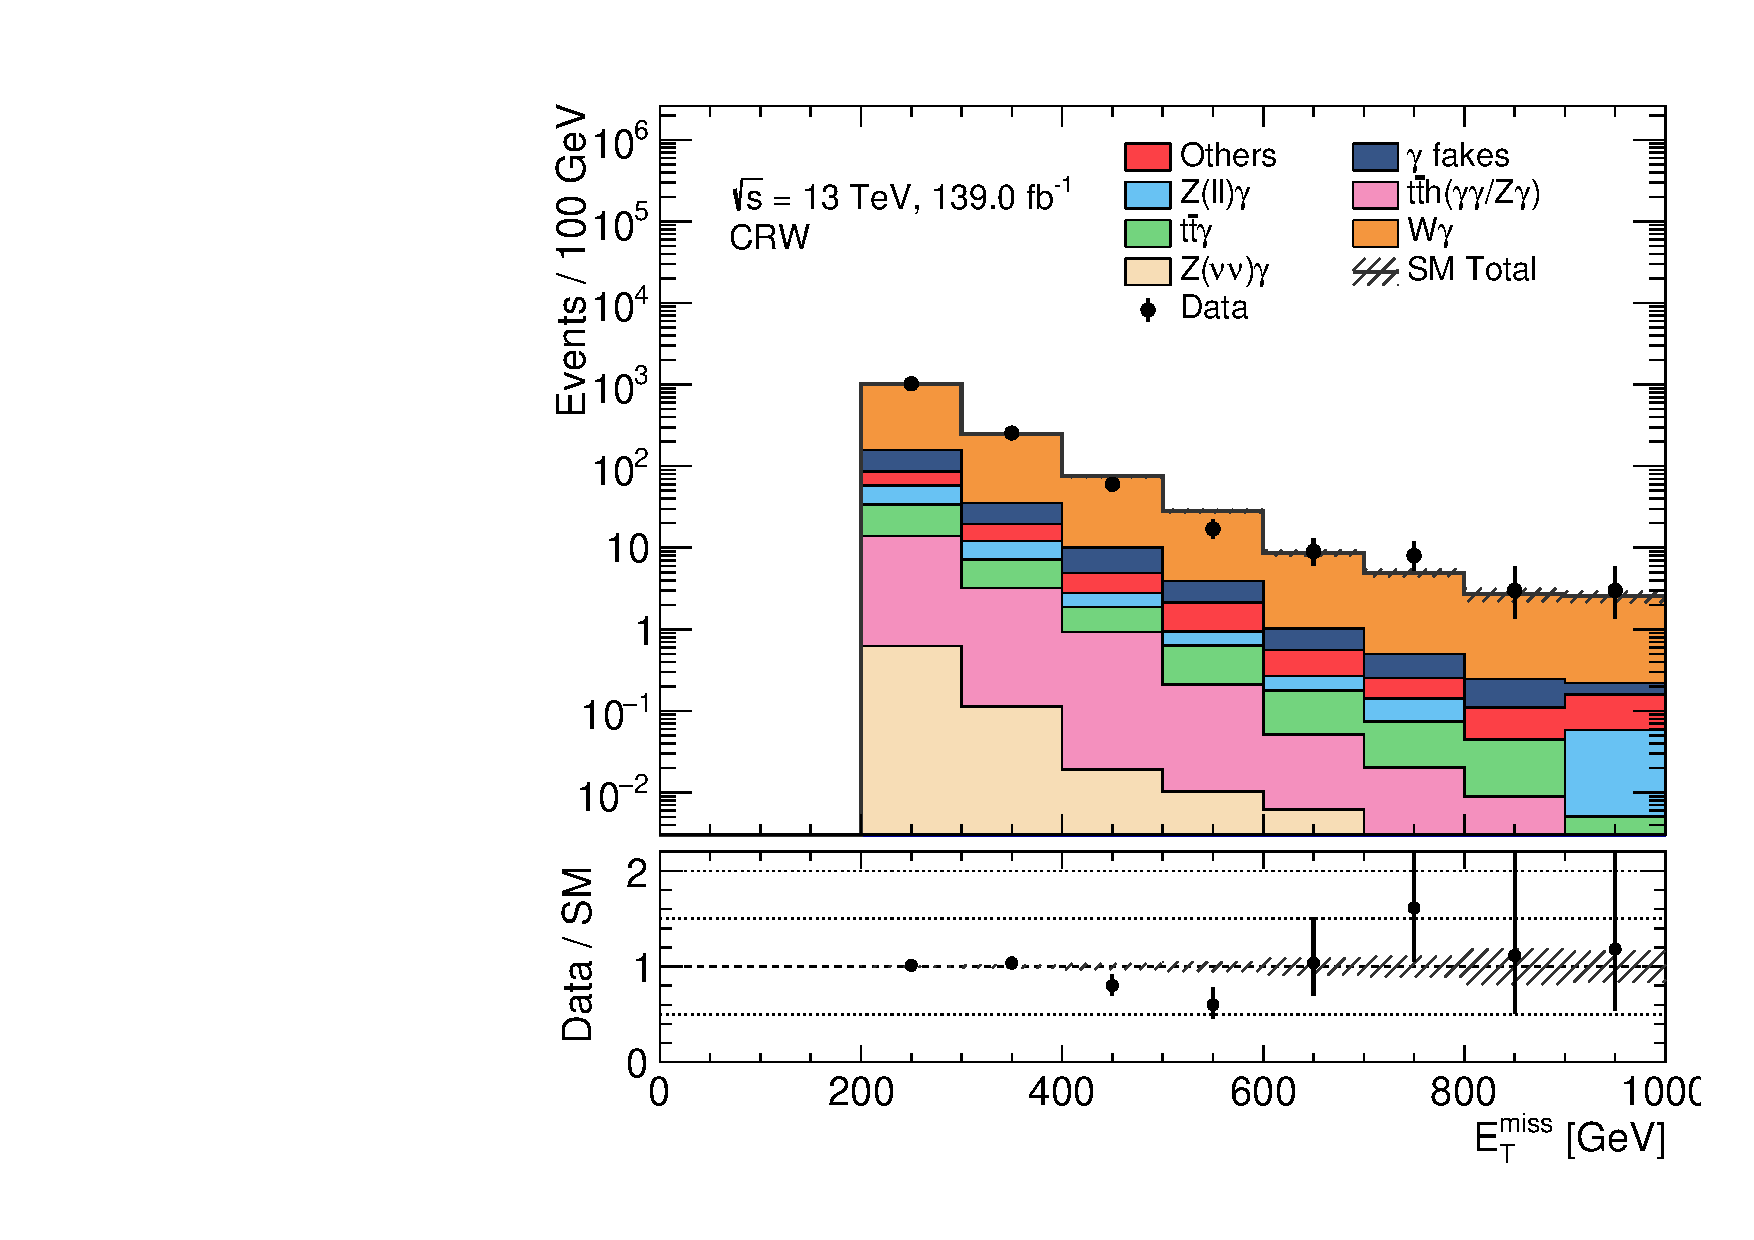
\includegraphics[width=0.32\textwidth]{images/analysis_EWK/v192_2_nosyst/can_CRW_met_et_afterFit.pdf}
    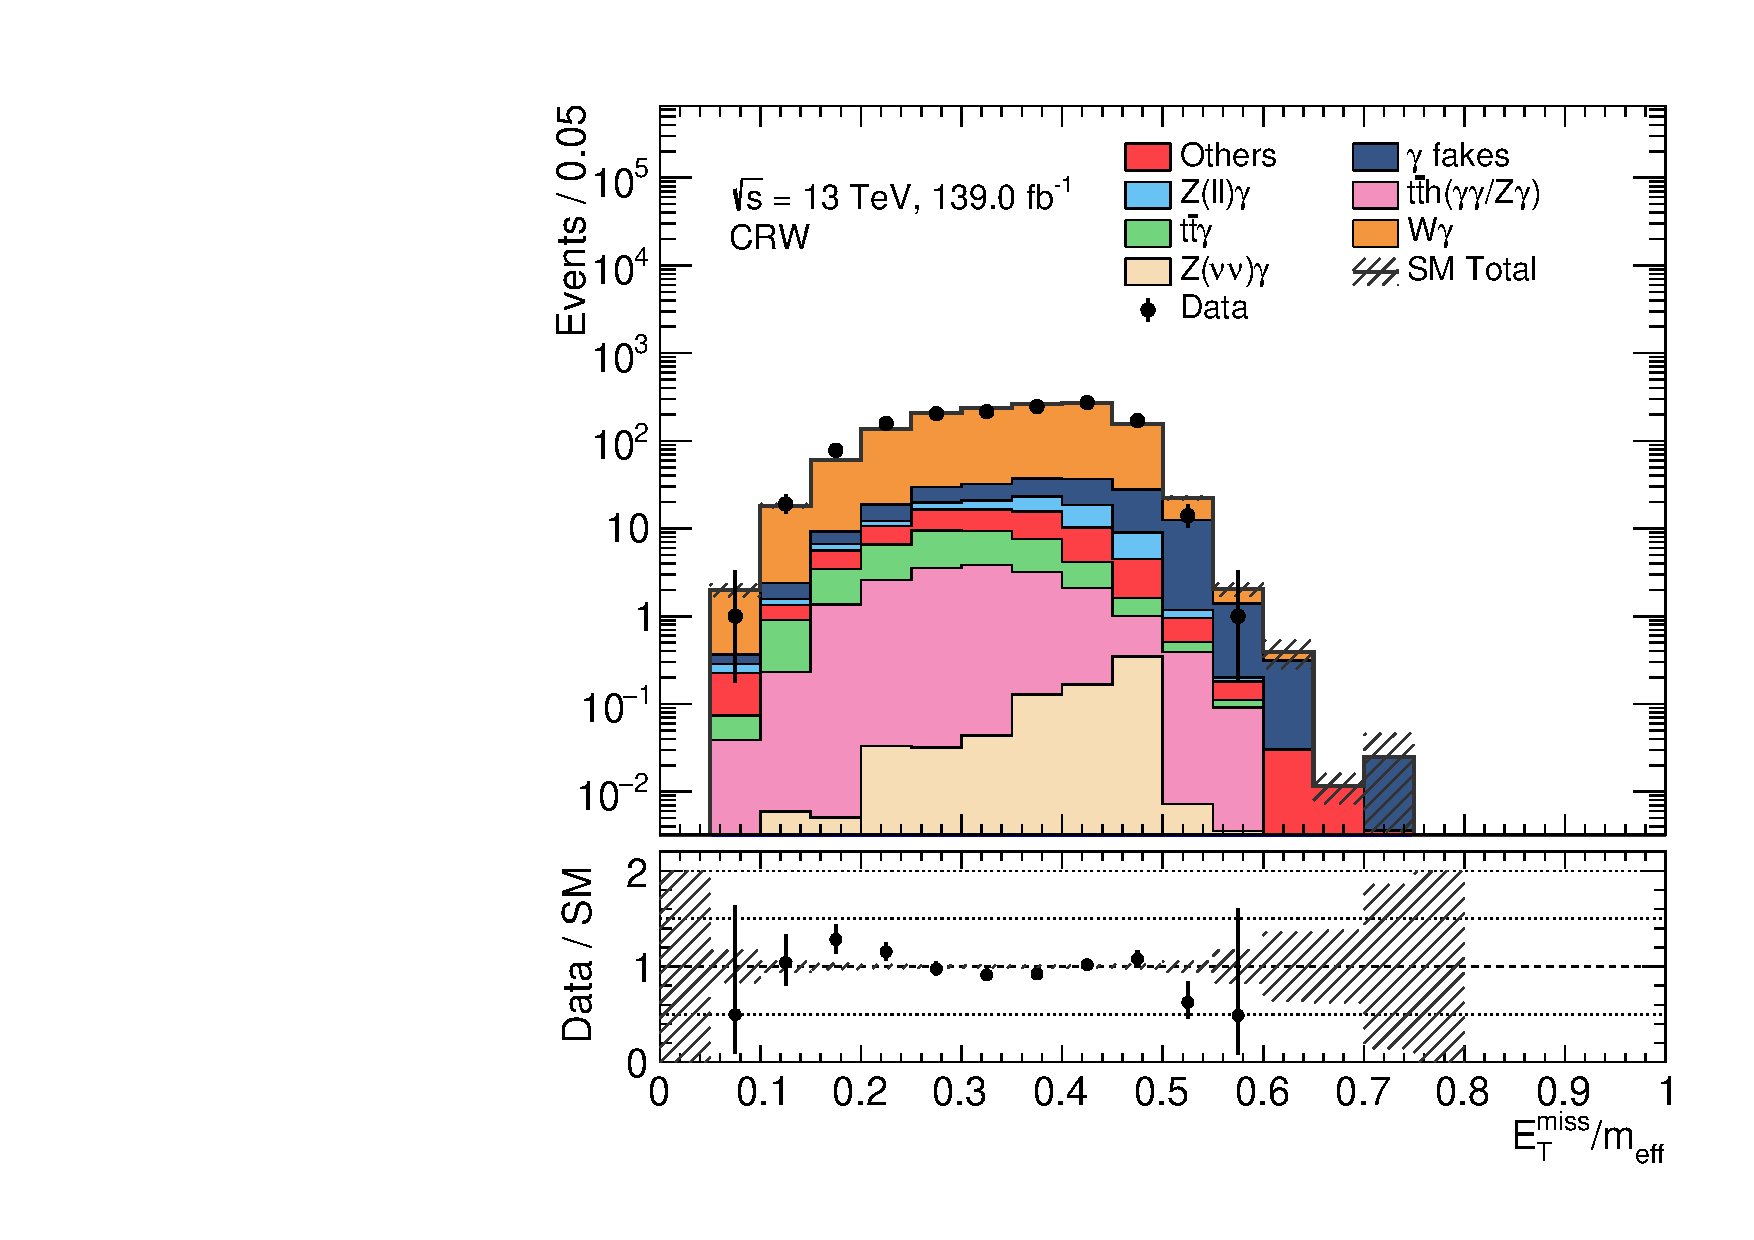
\includegraphics[width=0.32\textwidth]{images/analysis_EWK/v192_2_nosyst/can_CRW_met_etmeff_afterFit.pdf}
    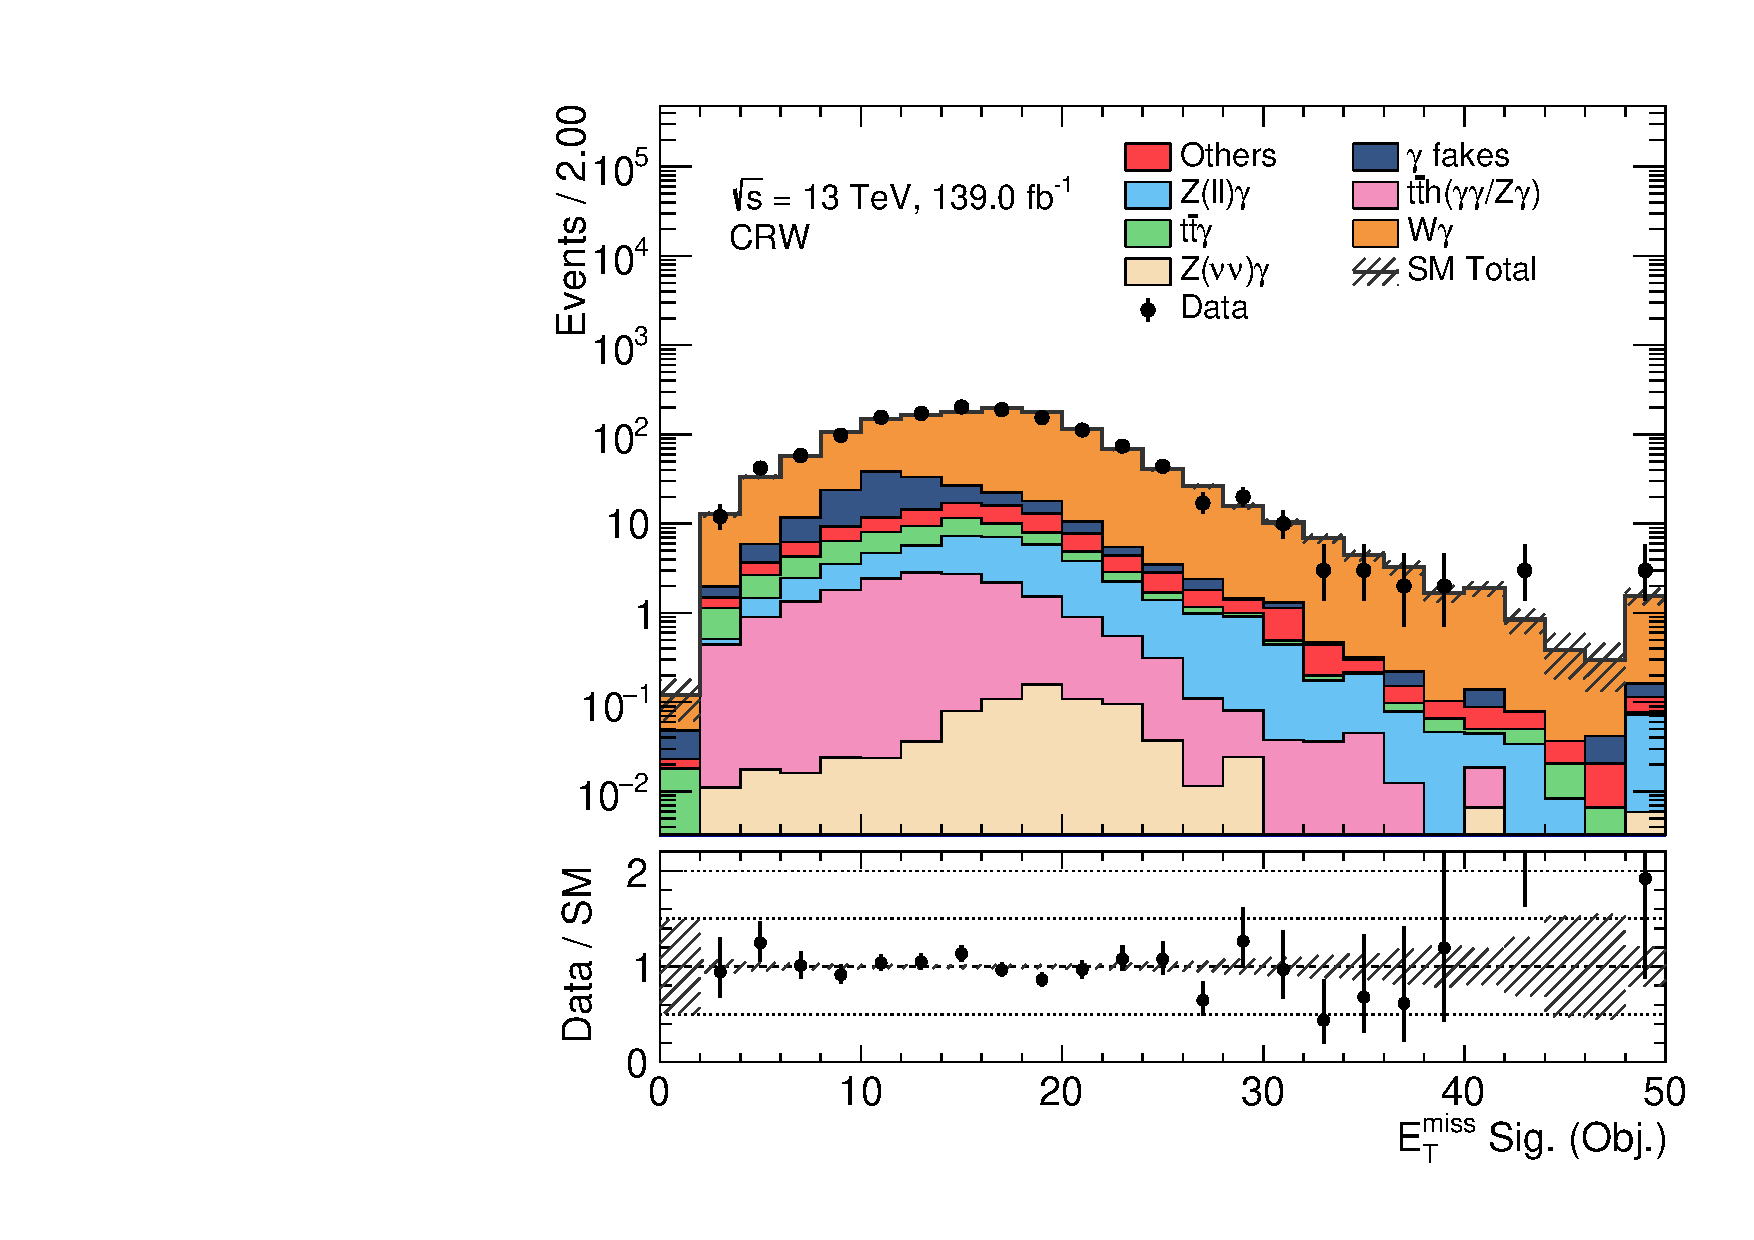
\includegraphics[width=0.32\textwidth]{images/analysis_EWK/v192_2_nosyst/can_CRW_met_sig_obj_afterFit.pdf}

    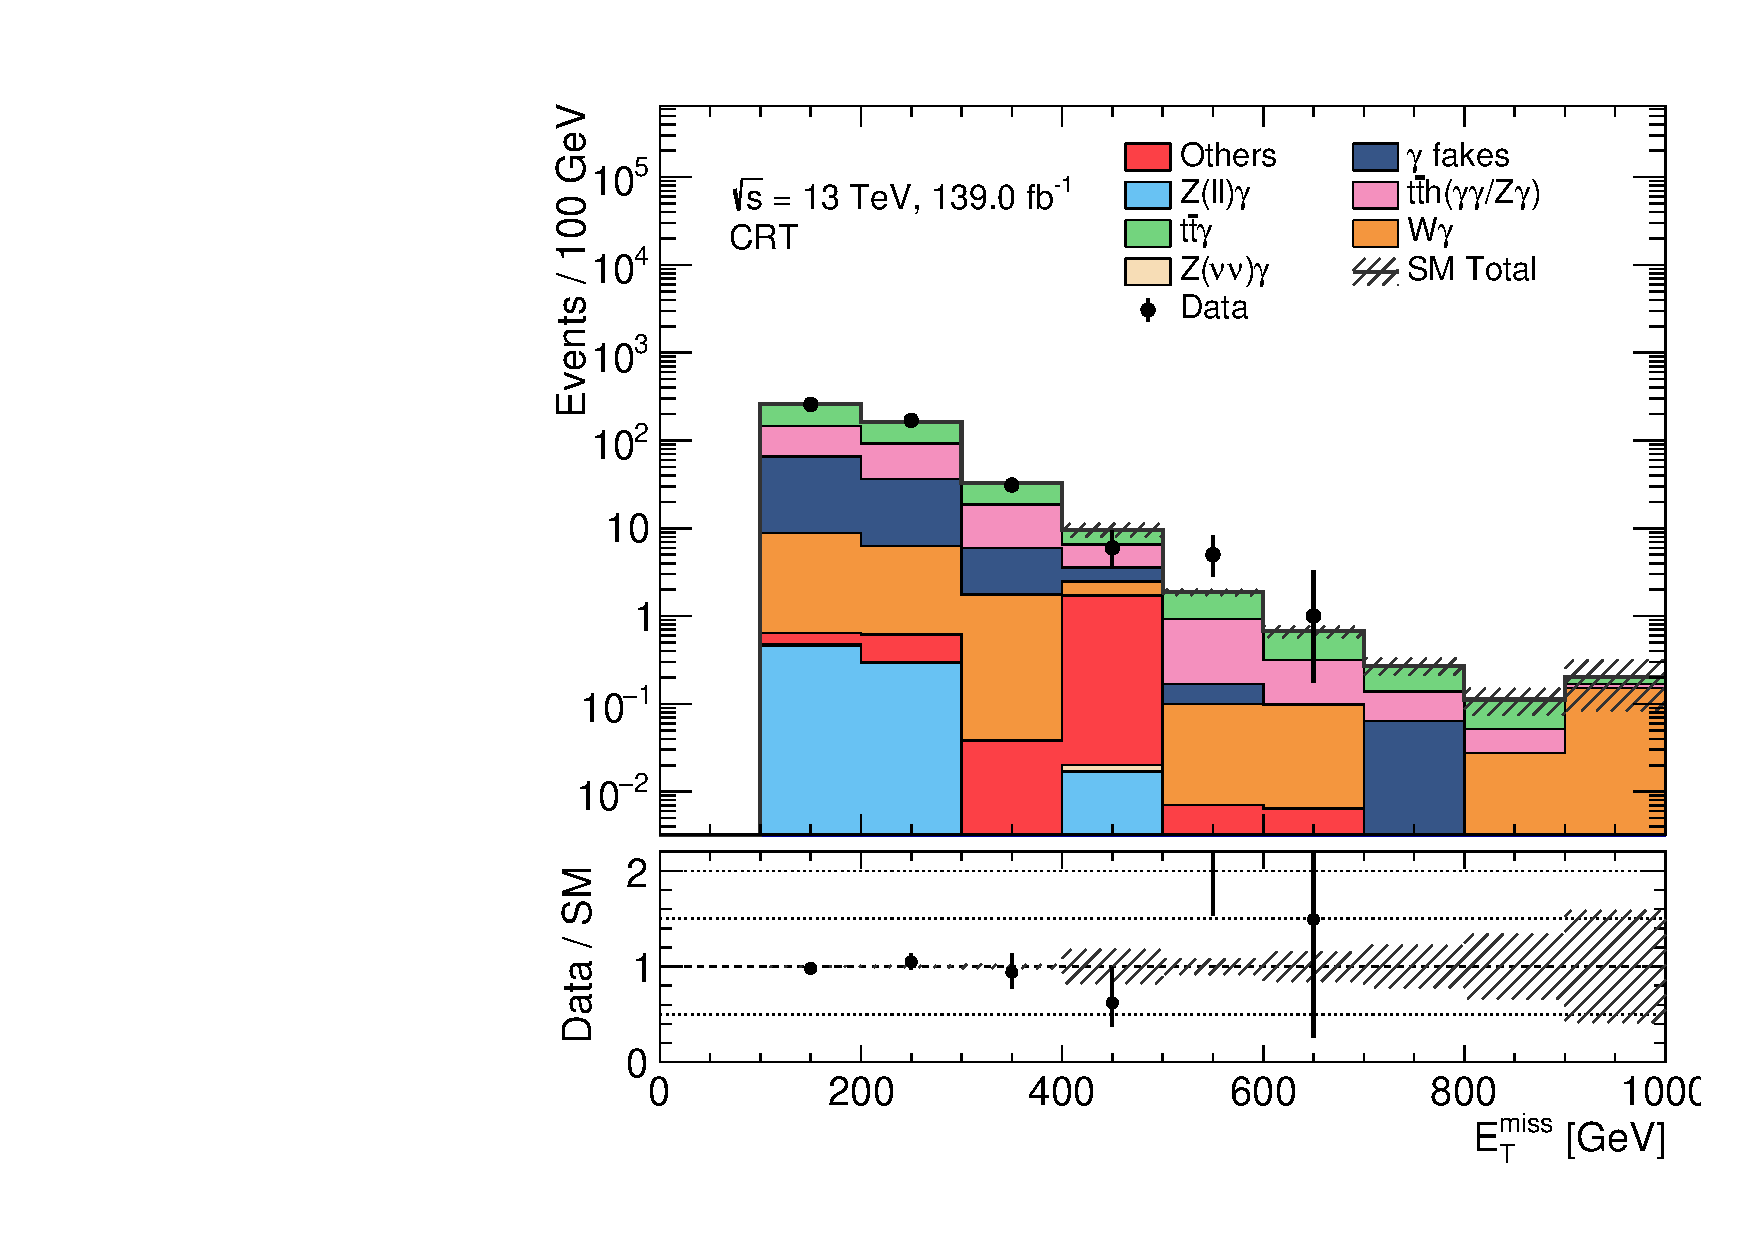
\includegraphics[width=0.32\textwidth]{images/analysis_EWK/v192_2_nosyst/can_CRT_met_et_afterFit.pdf}
    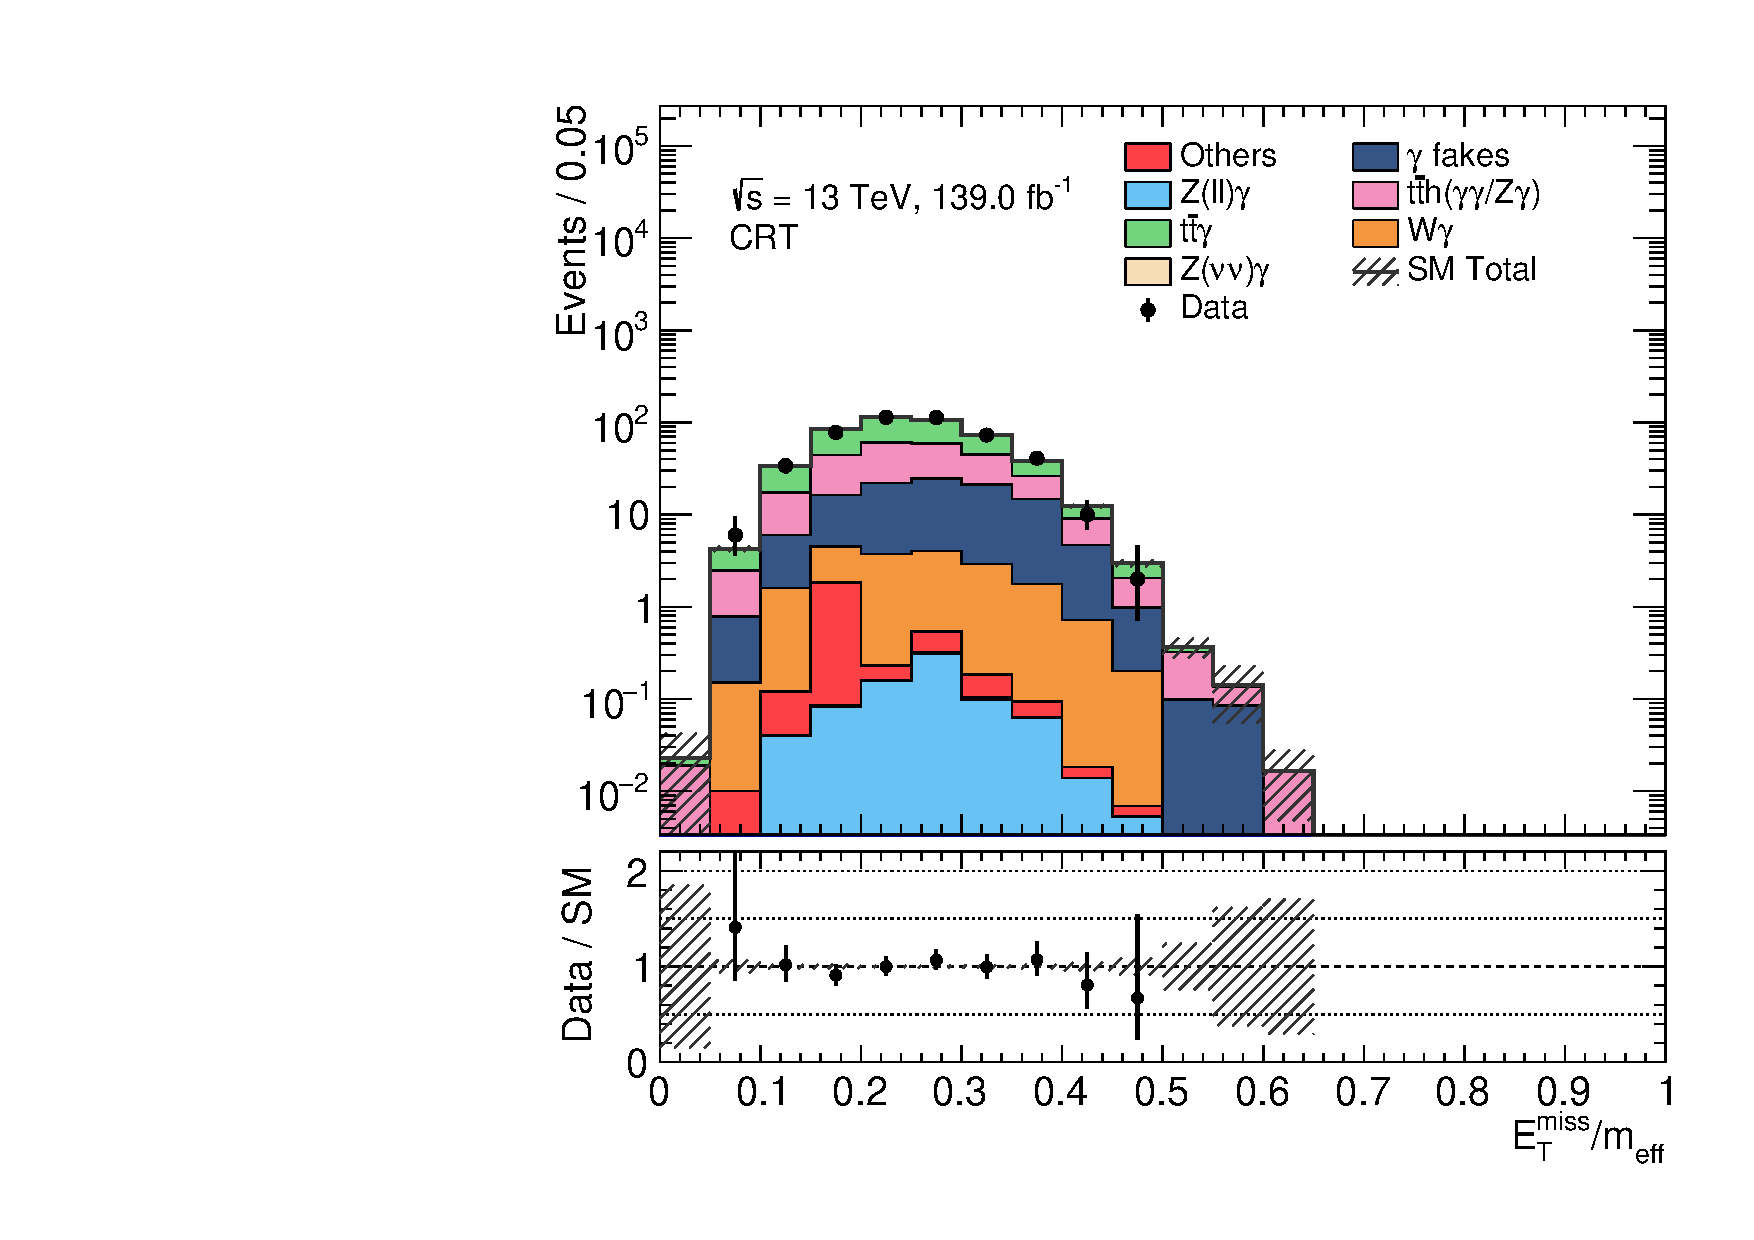
\includegraphics[width=0.32\textwidth]{images/analysis_EWK/v192_2_nosyst/can_CRT_met_etmeff_afterFit.pdf}
    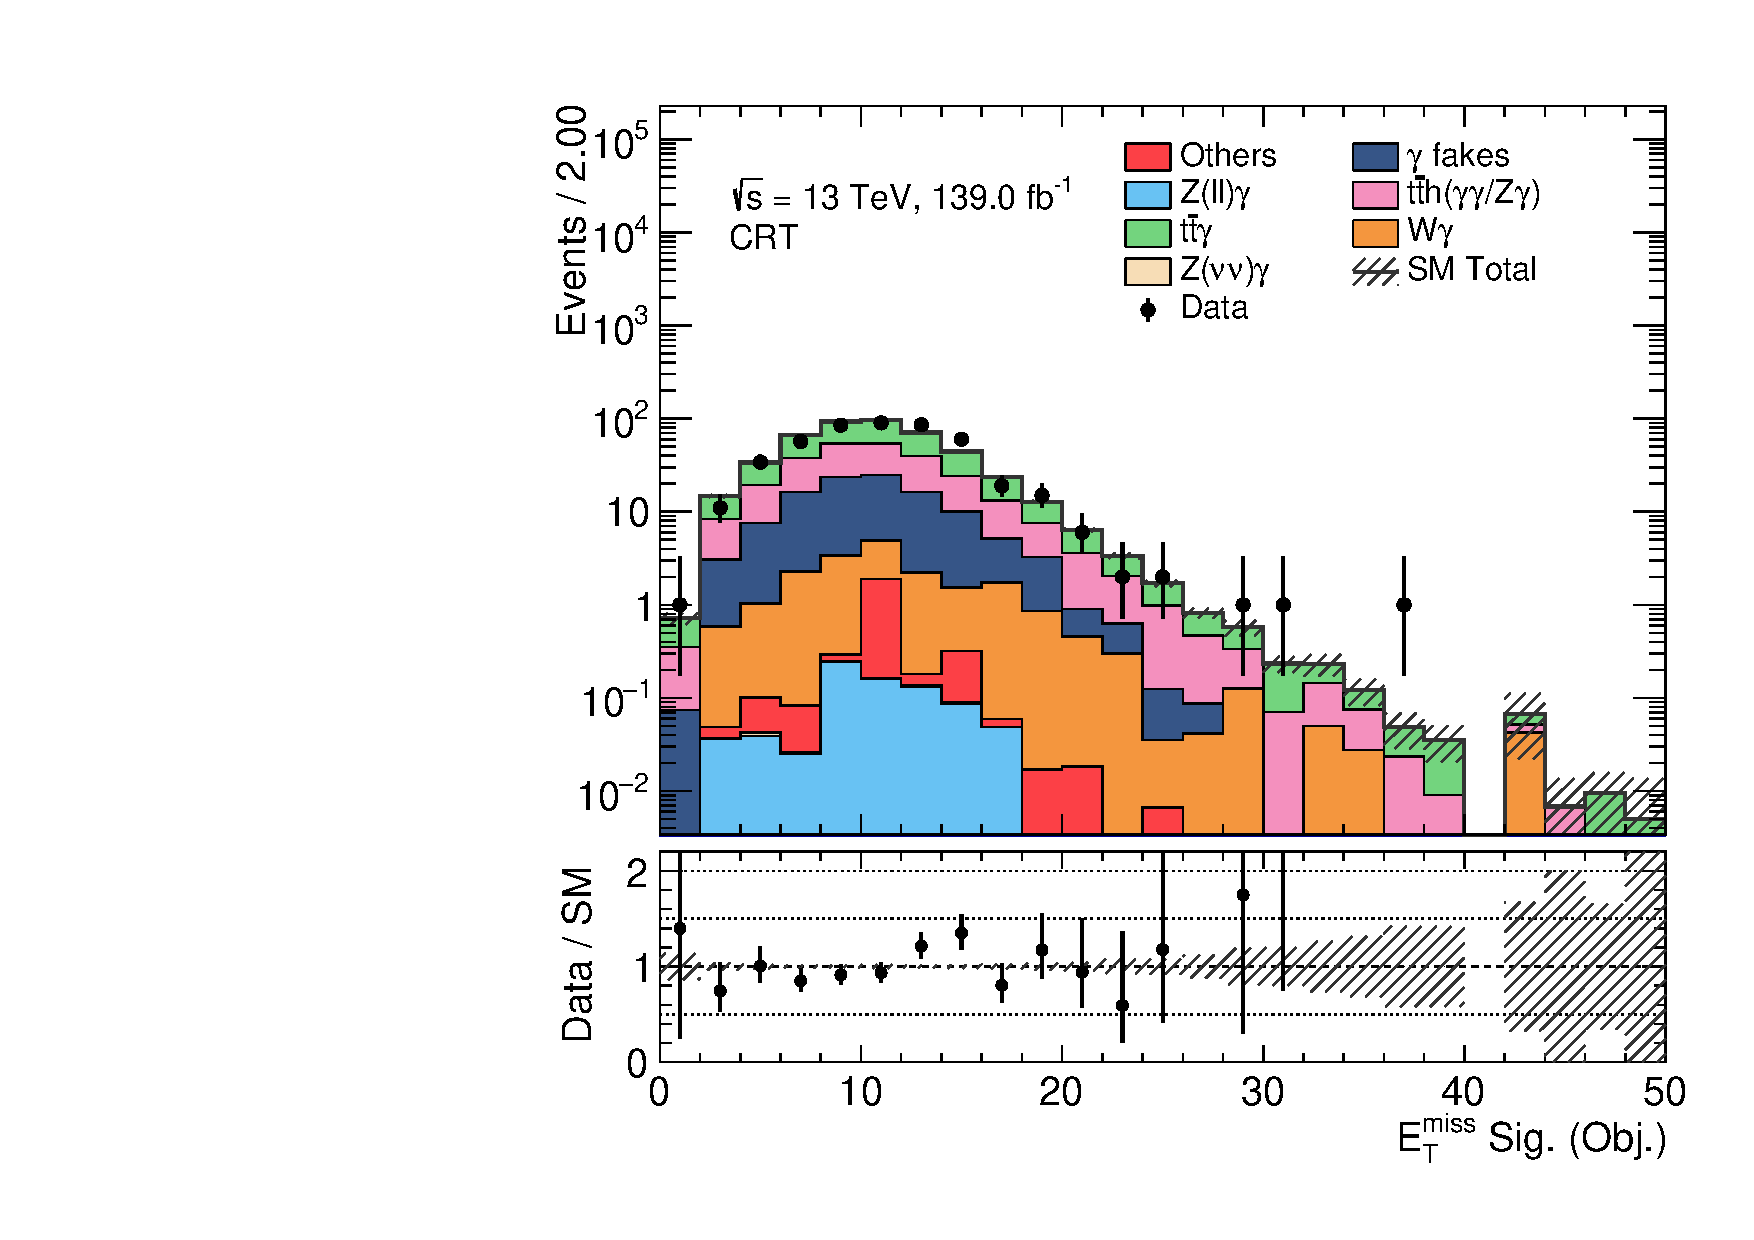
\includegraphics[width=0.32\textwidth]{images/analysis_EWK/v192_2_nosyst/can_CRT_met_sig_obj_afterFit.pdf}

    \caption{Distribuciones preliminares en la región de control CRW y CRT luego del ajuste de solo fondo, para el análisis de producción electrodébil. Las incertezas mostradas son sólo estadísticas.}
    \label{fig:crw_crt_dist_ewk}

\end{figure}


\begin{figure}

\centering
    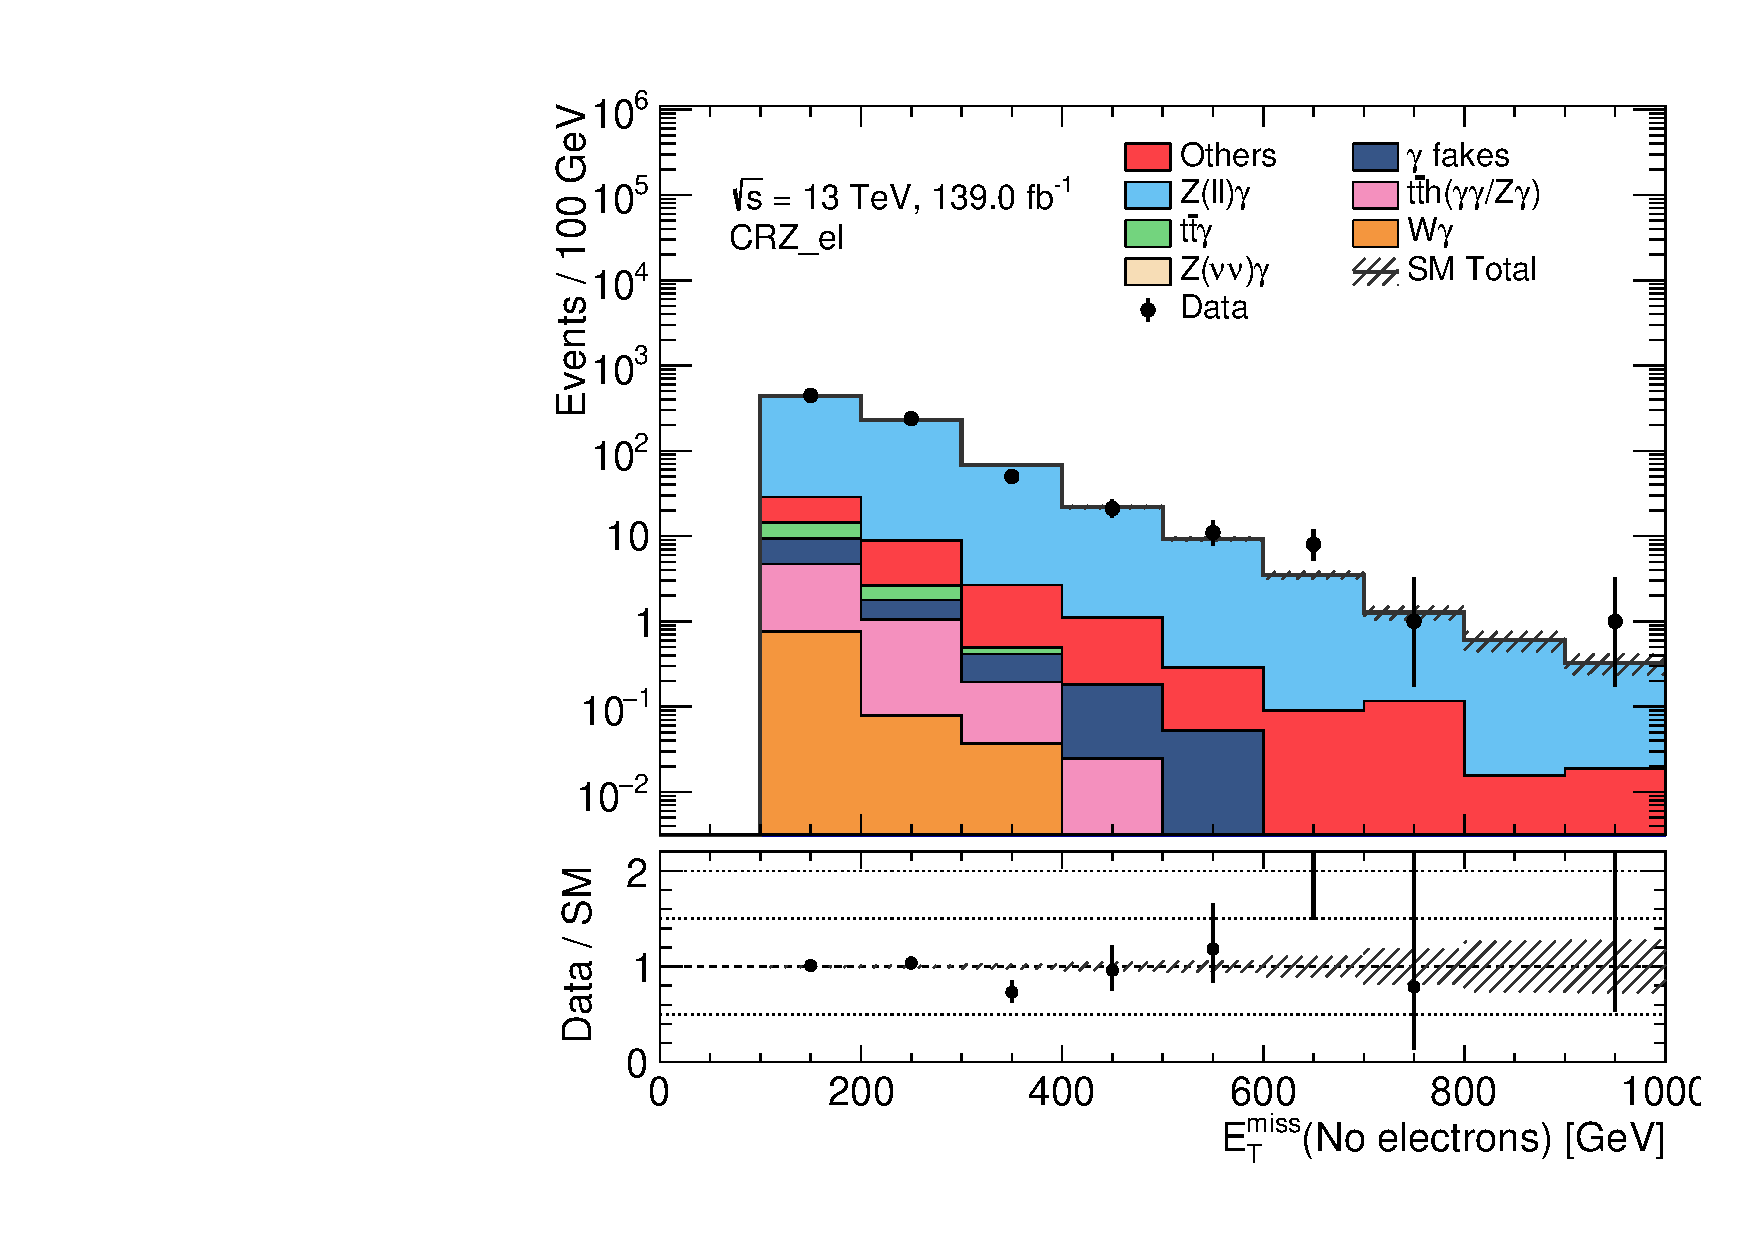
\includegraphics[width=0.49\textwidth]{images/analysis_EWK/v192_2_nosyst/can_CRZ_el_met_noele_et_afterFit.pdf}
    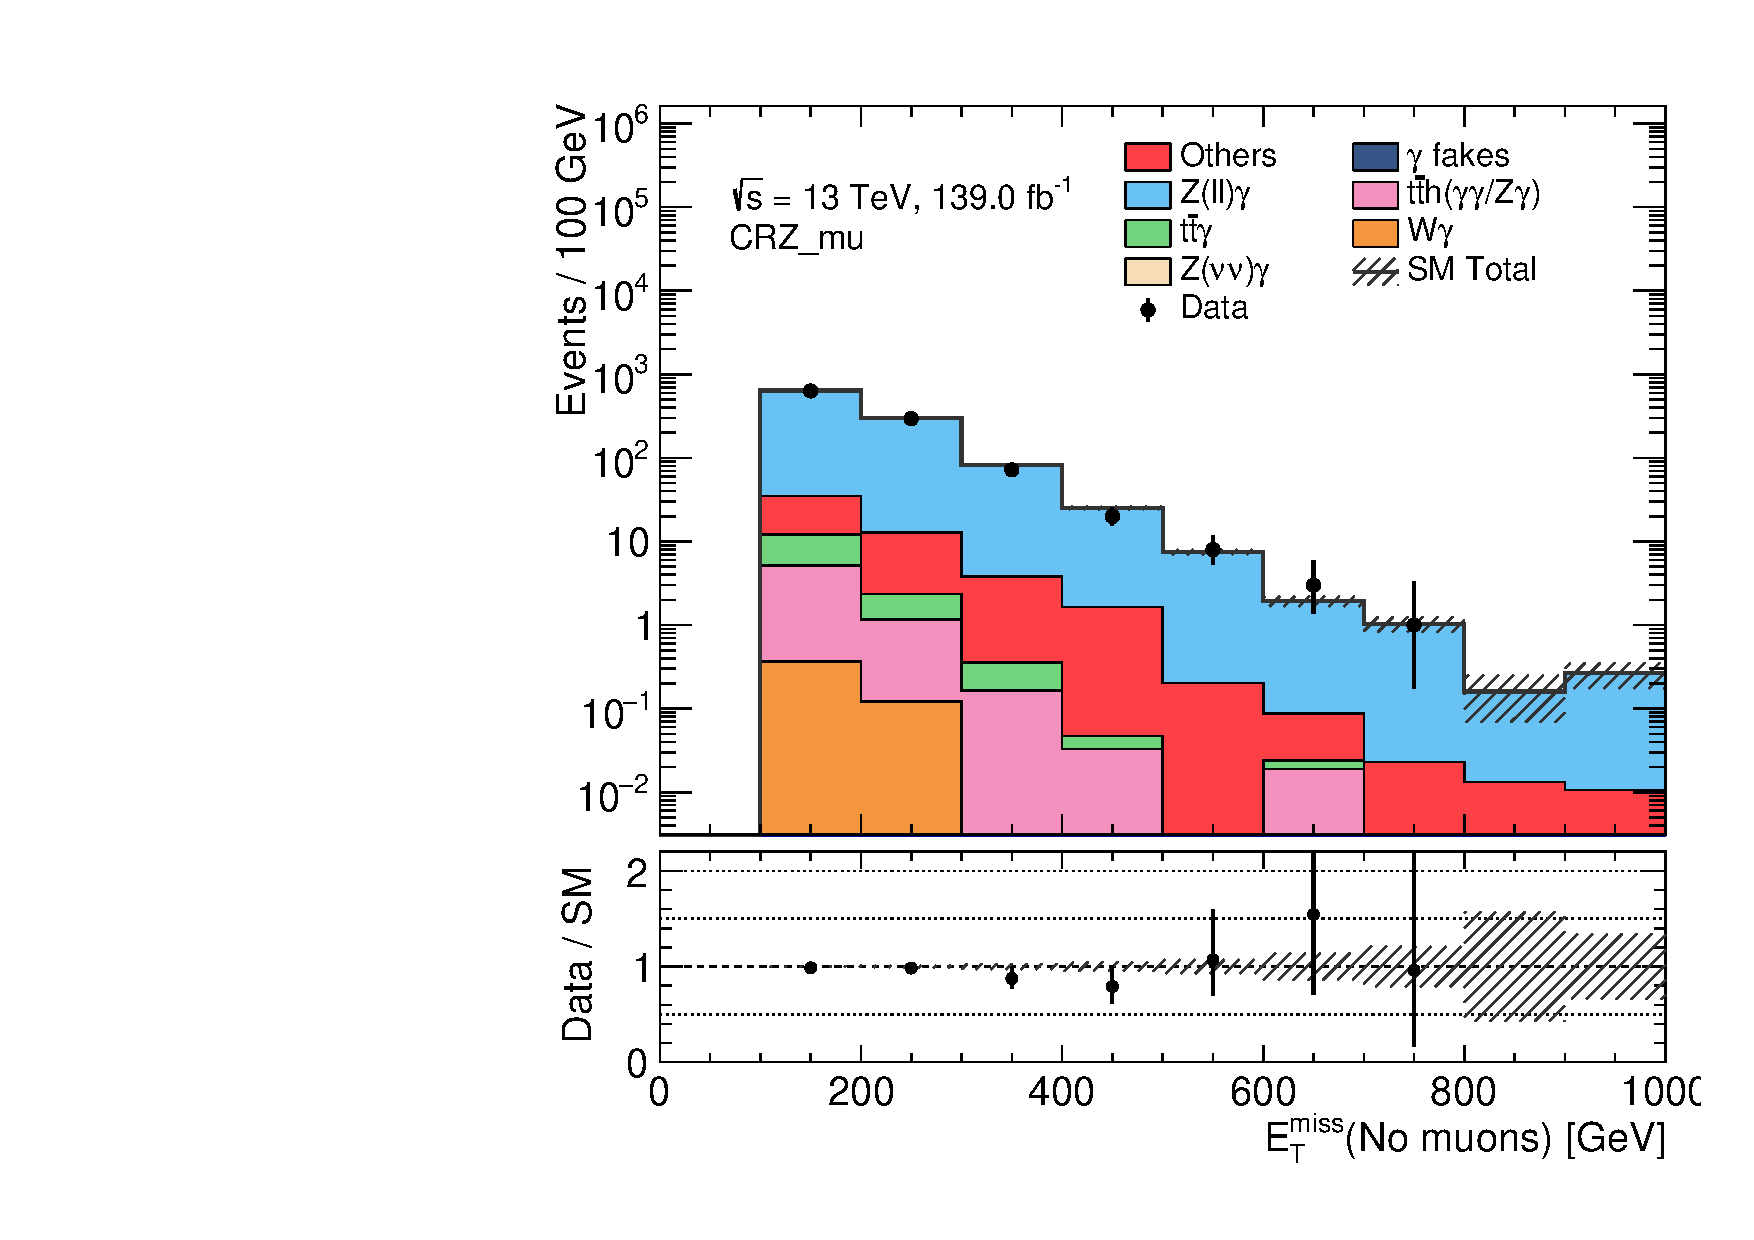
\includegraphics[width=0.49\textwidth]{images/analysis_EWK/v192_2_nosyst/can_CRZ_mu_met_nomuon_et_afterFit.pdf}

    \caption{Distribuciones preliminares de \met en las regiones de control CRZ\_el y CRZ\_mu luego del ajuste de solo fondo, para el análisis de producción electrodébil. En el cálculo de dicha variable se remueve los correspondientes leptones. Las incertezas mostradas son sólo estadísticas.}
    \label{fig:crz_el_mu_dist_ewk}
\end{figure}



En la Tabla \ref{tab:fit_result_vr} se muestran los resultados de las estimación de los fondos y su comparación con los datos en las regiones de validación, mientras que en la Figura \ref{fig:vr_ewk} se muestran algunas de las distribuciones más significativas. El acuerdo en dichas regiones se considera que es apropiado. 

\begin{table}[ht!]
  \centering
  \caption{Estimación preliminar de los fondos y de la señal en las distintas regiones de validación luego del ajuste de solo fondo para el análisis de producción electrodébil.}
  \resizebox{\textwidth}{!}{\begin{tabular}{lrrrrr}
\hline
Validation Regions & VRW & VRT & VRE & VRZee & VRZmm \\
\hline
Observed events & 1443 & 467 & 625 & 314 & 373 \\
\hline
Expected SM events & $1456.49 \pm 34.49$ & $428.91 \pm 16.42$ & $654.58 \pm 7.11$ & $309.18 \pm 8.26$ & $384.29 \pm 10.22$ \\
\hline
$Z(\nu\nu)\gamma$ & $1.24 \pm 0.03$ & $0.17 \pm 0.05$ & $10.42 \pm 2.66$ & $0.00 \pm 0.00$ & $0.00 \pm 0.00$ \\
$t\bar{t}\gamma$ & $106.74 \pm 6.46$ & $149.78 \pm 9.07$ & $1.73 \pm 0.27$ & $0.72 \pm 0.11$ & $0.98 \pm 0.14$ \\
$t\bar{t}h(\gamma\gamma/Z\gamma)$ & $89.51 \pm 5.42$ & $122.26 \pm 27.12$ & $2.08 \pm 0.39$ & $0.75 \pm 0.14$ & $0.84 \pm 0.15$ \\
$W\gamma$ & $1051.76 \pm 14.95$ & $74.70 \pm 2.38$ & $98.72 \pm 5.58$ & $0.08 \pm 0.00$ & $0.12 \pm 0.00$ \\
$Z(ll)\gamma$ & $30.89 \pm 5.12$ & $3.03 \pm 0.12$ & $0.48 \pm 0.03$ & $297.44 \pm 8.21$ & $367.64 \pm 10.13$ \\
$\gamma\ \text{fakes}$ & $135.70 \pm 9.87$ & $75.47 \pm 20.16$ & $517.95 \pm 109.31$ & $0.86 \pm 0.29$ & $0.00 \pm 0.00$ \\
Others & $40.64 \pm 5.31$ & $3.49 \pm 1.01$ & $23.20 \pm 4.21$ & $9.33 \pm 1.86$ & $14.72 \pm 2.93$ \\
\hline
 &  &  &  &  &  \\
\hline
$\gamma+Z, m_{\tilde{\chi}_{1}^{0}} = 150 \text{GeV}$ & $ 100.60 \pm 12.88 (6.91\%)$ & $ 2.78 \pm 1.99 (0.65\%)$ & $ 55.94 \pm 10.56 (8.55\%)$ & $ 7.22 \pm 3.25 (2.33\%)$ & $ 14.73 \pm 4.52 (3.83\%)$ \\
$\gamma+Z, m_{\tilde{\chi}_{1}^{0}} = 250 \text{GeV}$ & $ 131.45 \pm 5.88 (9.02\%)$ & $ 16.24 \pm 2.21 (3.79\%)$ & $ 24.58 \pm 2.57 (3.75\%)$ & $ 4.20 \pm 1.01 (1.36\%)$ & $ 3.51 \pm 0.92 (0.91\%)$ \\
$\gamma+Z, m_{\tilde{\chi}_{1}^{0}} = 350 \text{GeV}$ & $ 88.95 \pm 2.59 (6.11\%)$ & $ 12.02 \pm 0.94 (2.80\%)$ & $ 11.25 \pm 0.95 (1.72\%)$ & $ 1.18 \pm 0.29 (0.38\%)$ & $ 1.52 \pm 0.32 (0.40\%)$ \\
$\gamma+Z, m_{\tilde{\chi}_{1}^{0}} = 450 \text{GeV}$ & $ 48.33 \pm 2.27 (3.32\%)$ & $ 7.54 \pm 0.88 (1.76\%)$ & $ 7.32 \pm 0.91 (1.12\%)$ & $ 0.19 \pm 0.14 (0.06\%)$ & $ 0.28 \pm 0.16 (0.07\%)$ \\
$\gamma+Z, m_{\tilde{\chi}_{1}^{0}} = 550 \text{GeV}$ & $ 24.77 \pm 1.59 (1.70\%)$ & $ 3.65 \pm 0.61 (0.85\%)$ & $ 2.72 \pm 0.57 (0.42\%)$ & $ 0.30 \pm 0.18 (0.10\%)$ & $ 0.14 \pm 0.10 (0.04\%)$ \\
$\gamma+Z, m_{\tilde{\chi}_{1}^{0}} = 650 \text{GeV}$ & $ 11.96 \pm 0.99 (0.82\%)$ & $ 1.70 \pm 0.38 (0.40\%)$ & $ 1.51 \pm 0.35 (0.23\%)$ & $ 0.00 \pm 0.00 (0.00\%)$ & $ 0.07 \pm 0.07 (0.02\%)$ \\
$\gamma+Z, m_{\tilde{\chi}_{1}^{0}} = 750 \text{GeV}$ & $ 5.86 \pm 0.56 (0.40\%)$ & $ 0.92 \pm 0.24 (0.21\%)$ & $ 1.03 \pm 0.23 (0.16\%)$ & $ 0.00 \pm 0.00 (0.00\%)$ & $ 0.00 \pm 0.00 (0.00\%)$ \\
\hline
% $\gamma+Z, m_{\tilde{\chi}_{1}^{0}} = 850 \text{GeV}$ & $ 2.85 \pm 0.28 (0.20\%)$ & $ 0.36 \pm 0.10 (0.08\%)$ & $ 0.57 \pm 0.13 (0.09\%)$ & $ 0.00 \pm 0.00 (0.00\%)$ & $ 0.00 \pm 0.00 (0.00\%)$ \\
$\gamma+h, m_{\tilde{\chi}_{1}^{0}} = 150 \text{GeV}$ & $ 87.28 \pm 12.86 (5.99\%)$ & $ 15.08 \pm 4.99 (3.52\%)$ & $ 58.40 \pm 9.98 (8.92\%)$ & $ 0.00 \pm 0.00 (0.00\%)$ & $ 0.00 \pm 0.00 (0.00\%)$ \\
$\gamma+h, m_{\tilde{\chi}_{1}^{0}} = 250 \text{GeV}$ & $ 149.13 \pm 6.13 (10.24\%)$ & $ 29.70 \pm 2.76 (6.92\%)$ & $ 24.55 \pm 2.62 (3.75\%)$ & $ 0.00 \pm 0.00 (0.00\%)$ & $ 0.00 \pm 0.00 (0.00\%)$ \\
$\gamma+h, m_{\tilde{\chi}_{1}^{0}} = 350 \text{GeV}$ & $ 144.26 \pm 3.30 (9.90\%)$ & $ 29.83 \pm 1.50 (6.96\%)$ & $ 10.18 \pm 0.92 (1.55\%)$ & $ 0.00 \pm 0.00 (0.00\%)$ & $ 0.00 \pm 0.00 (0.00\%)$ \\
$\gamma+h, m_{\tilde{\chi}_{1}^{0}} = 450 \text{GeV}$ & $ 82.61 \pm 2.94 (5.67\%)$ & $ 17.07 \pm 1.32 (3.98\%)$ & $ 5.21 \pm 0.75 (0.80\%)$ & $ 0.00 \pm 0.00 (0.00\%)$ & $ 0.11 \pm 0.11 (0.03\%)$ \\
$\gamma+h, m_{\tilde{\chi}_{1}^{0}} = 550 \text{GeV}$ & $ 42.02 \pm 2.06 (2.89\%)$ & $ 9.81 \pm 0.99 (2.29\%)$ & $ 4.31 \pm 0.68 (0.66\%)$ & $ 0.00 \pm 0.00 (0.00\%)$ & $ 0.00 \pm 0.00 (0.00\%)$ \\
$\gamma+h, m_{\tilde{\chi}_{1}^{0}} = 650 \text{GeV}$ & $ 24.15 \pm 1.42 (1.66\%)$ & $ 5.48 \pm 0.68 (1.28\%)$ & $ 1.94 \pm 0.41 (0.30\%)$ & $ 0.00 \pm 0.00 (0.00\%)$ & $ 0.00 \pm 0.00 (0.00\%)$ \\
$\gamma+h, m_{\tilde{\chi}_{1}^{0}} = 750 \text{GeV}$ & $ 10.26 \pm 0.75 (0.70\%)$ & $ 2.20 \pm 0.35 (0.51\%)$ & $ 1.31 \pm 0.26 (0.20\%)$ & $ 0.00 \pm 0.00 (0.00\%)$ & $ 0.00 \pm 0.00 (0.00\%)$ \\
% $\gamma+h, m_{\tilde{\chi}_{1}^{0}} = 850 \text{GeV}$ & $ 6.60 \pm 0.44 (0.45\%)$ & $ 1.12 \pm 0.19 (0.26\%)$ & $ 0.47 \pm 0.12 (0.07\%)$ & $ 0.00 \pm 0.00 (0.00\%)$ & $ 0.00 \pm 0.00 (0.00\%)$ \\
\hline
\end{tabular}
}
  \label{tab:fit_result_vr}
\end{table}


\begin{figure}

    \centering

    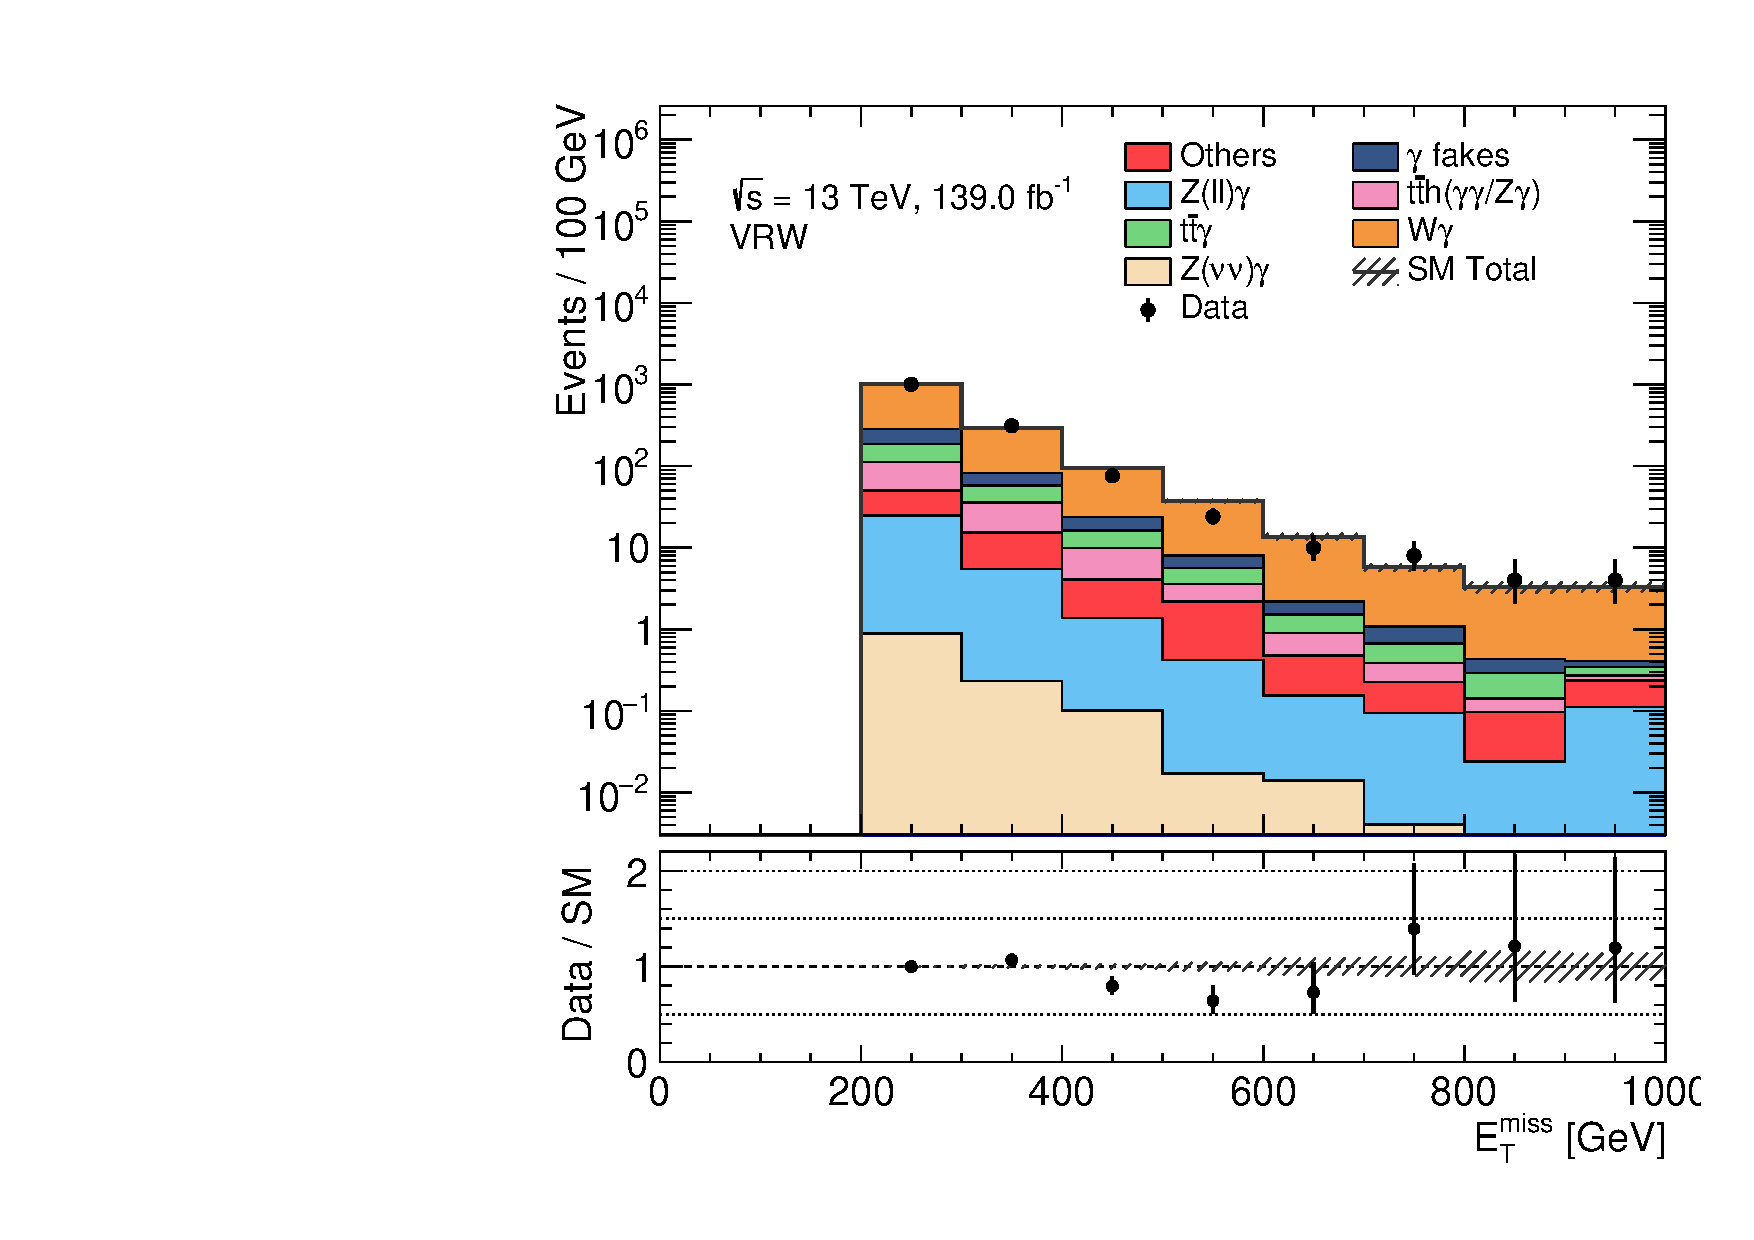
\includegraphics[width=0.24\textwidth]{images/analysis_EWK/v192_2_nosyst/can_VRW_met_et_afterFit.pdf}
    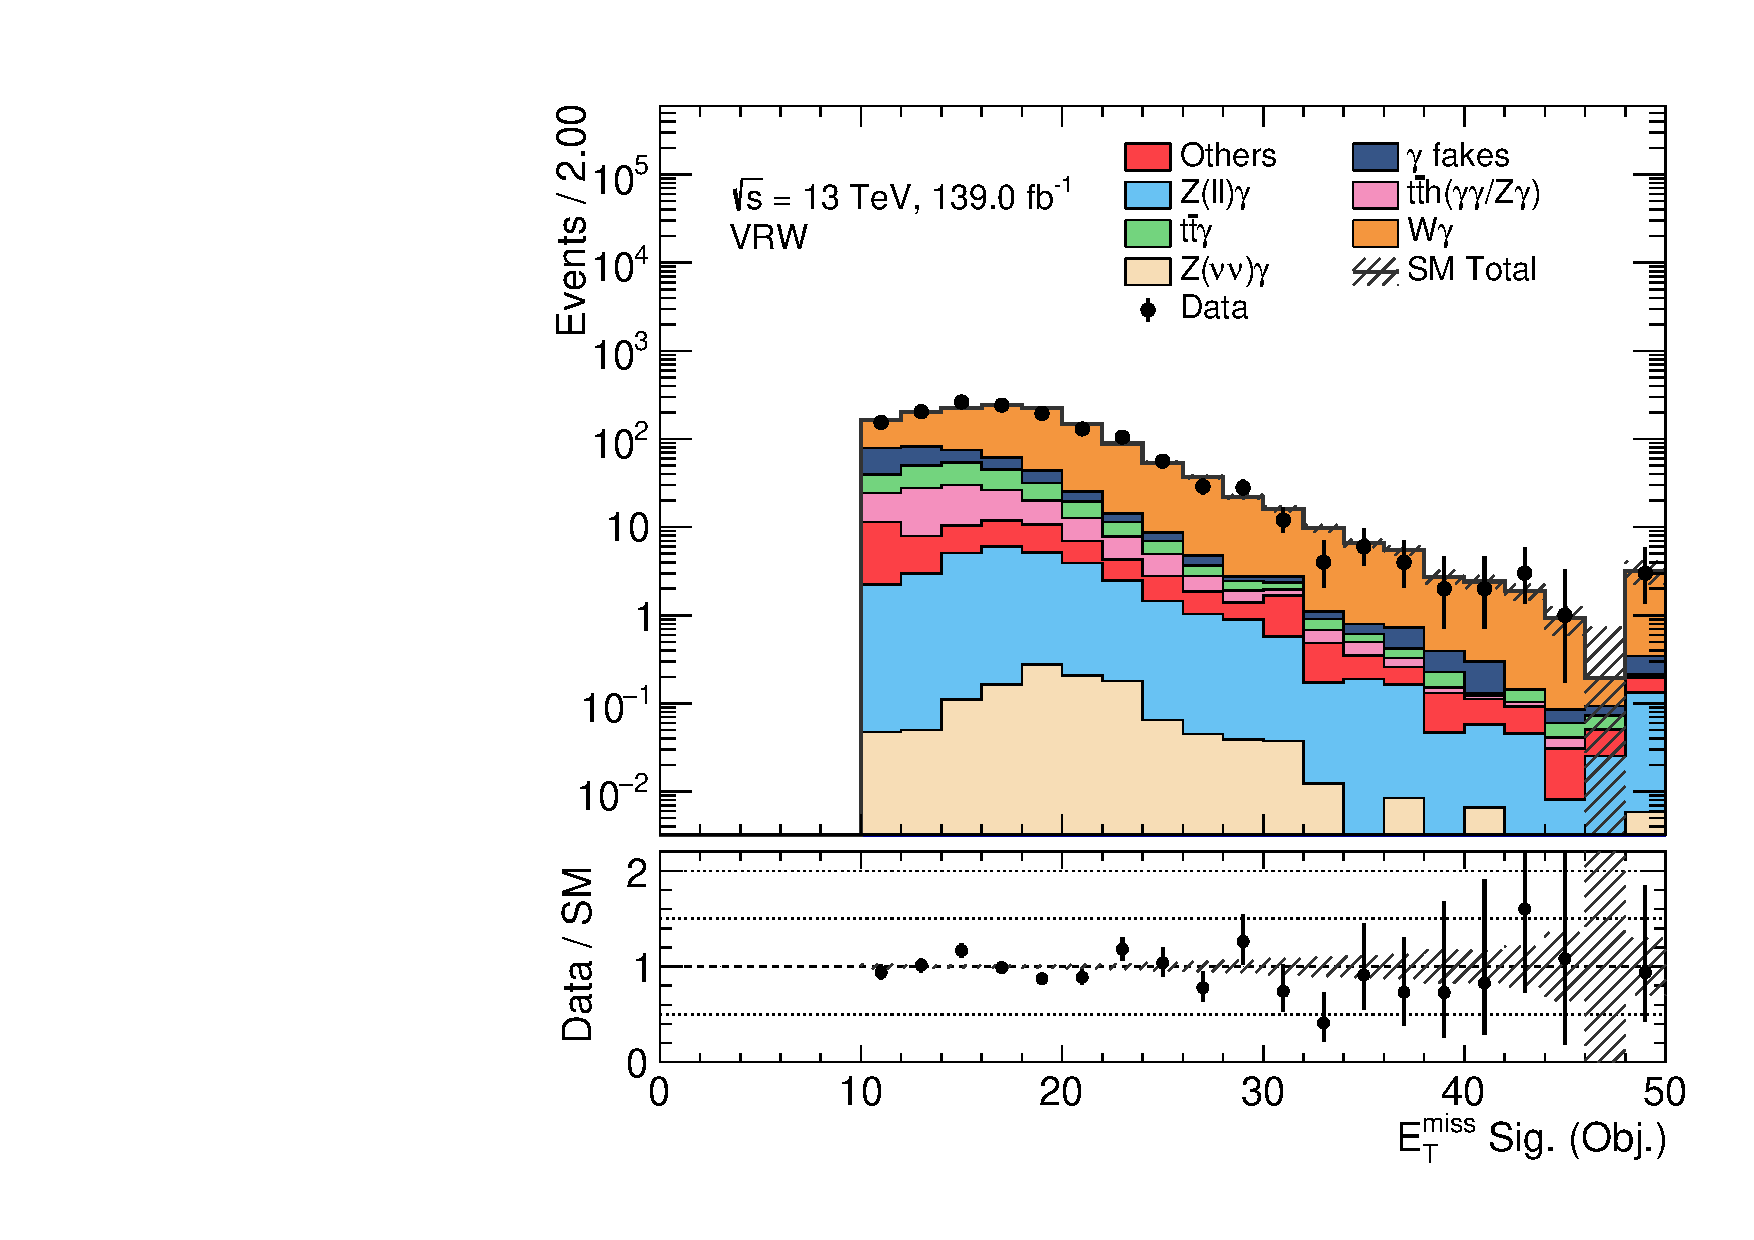
\includegraphics[width=0.24\textwidth]{images/analysis_EWK/v192_2_nosyst/can_VRW_met_sig_obj_afterFit.pdf}
    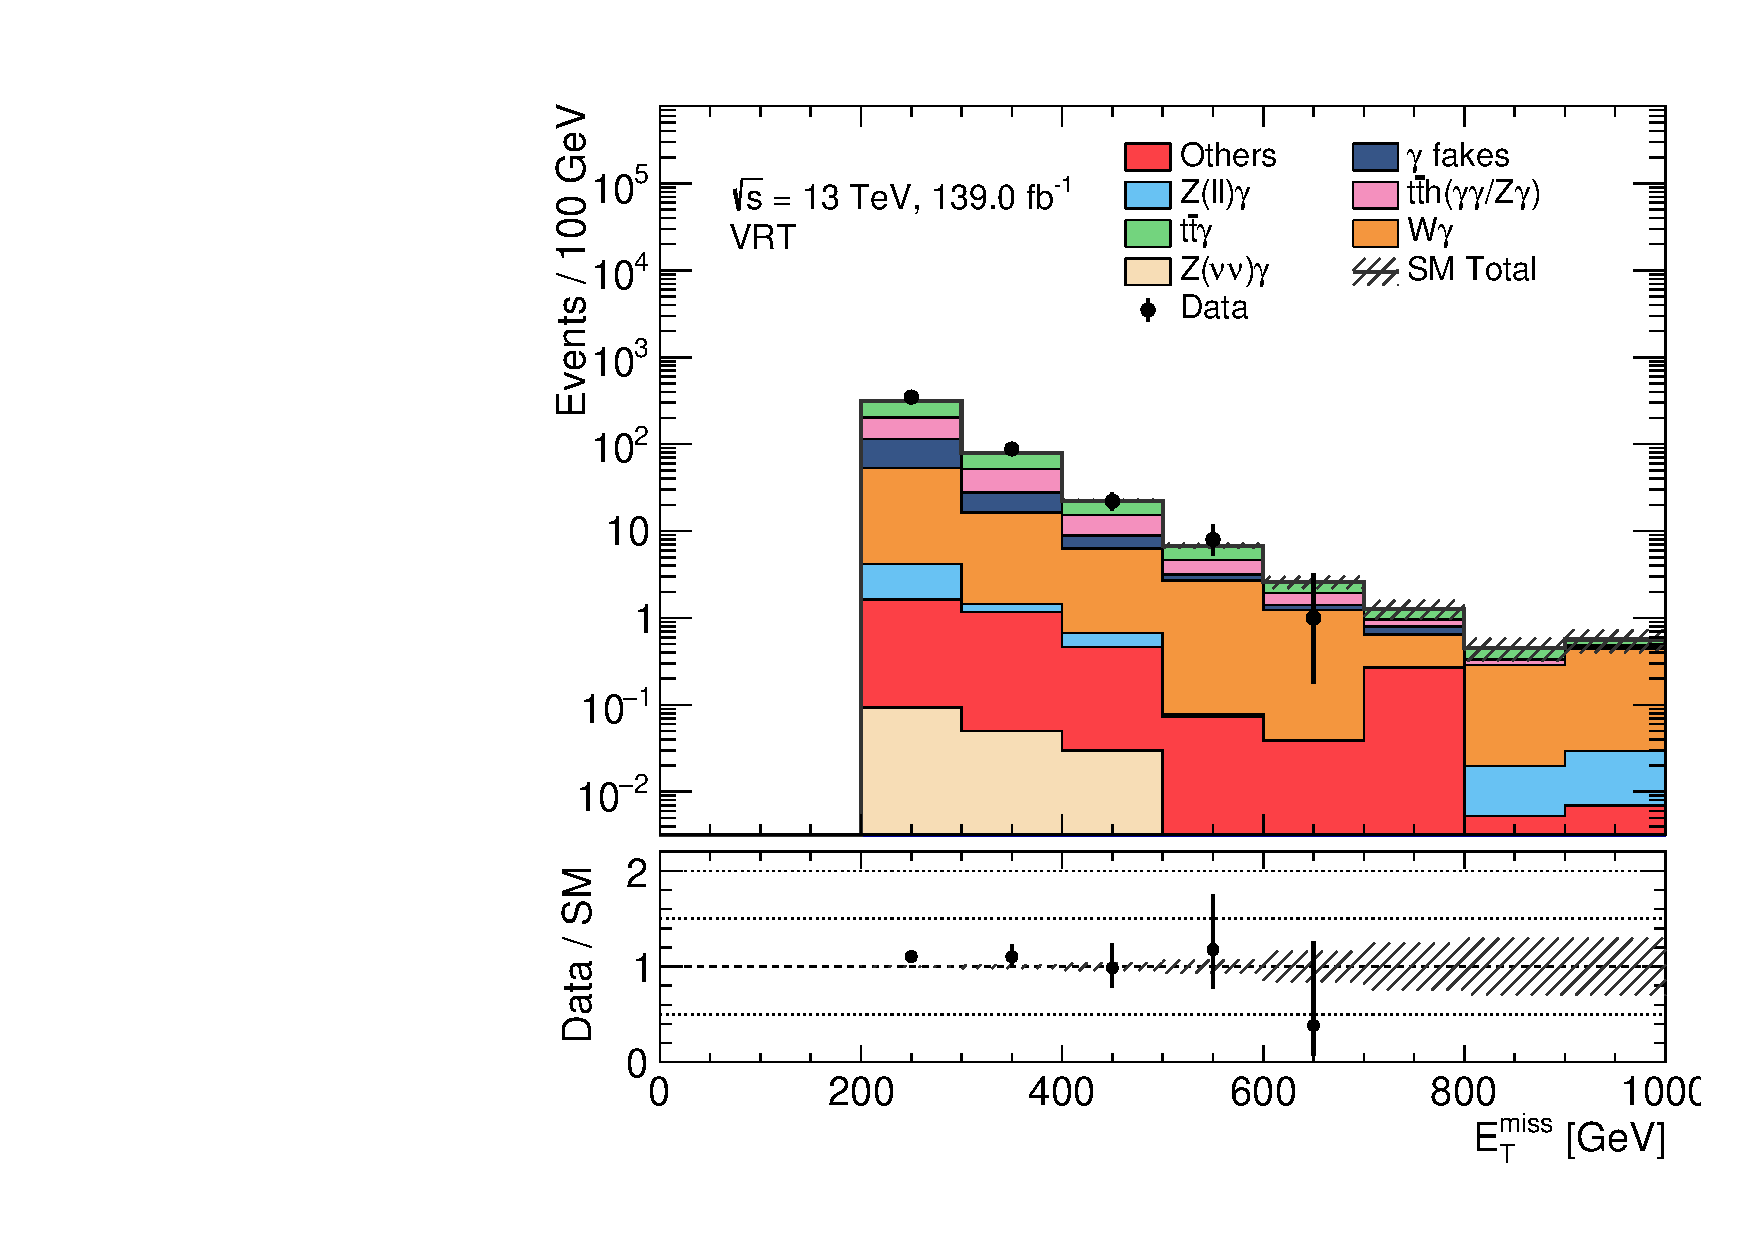
\includegraphics[width=0.24\textwidth]{images/analysis_EWK/v192_2_nosyst/can_VRT_met_et_afterFit.pdf}
    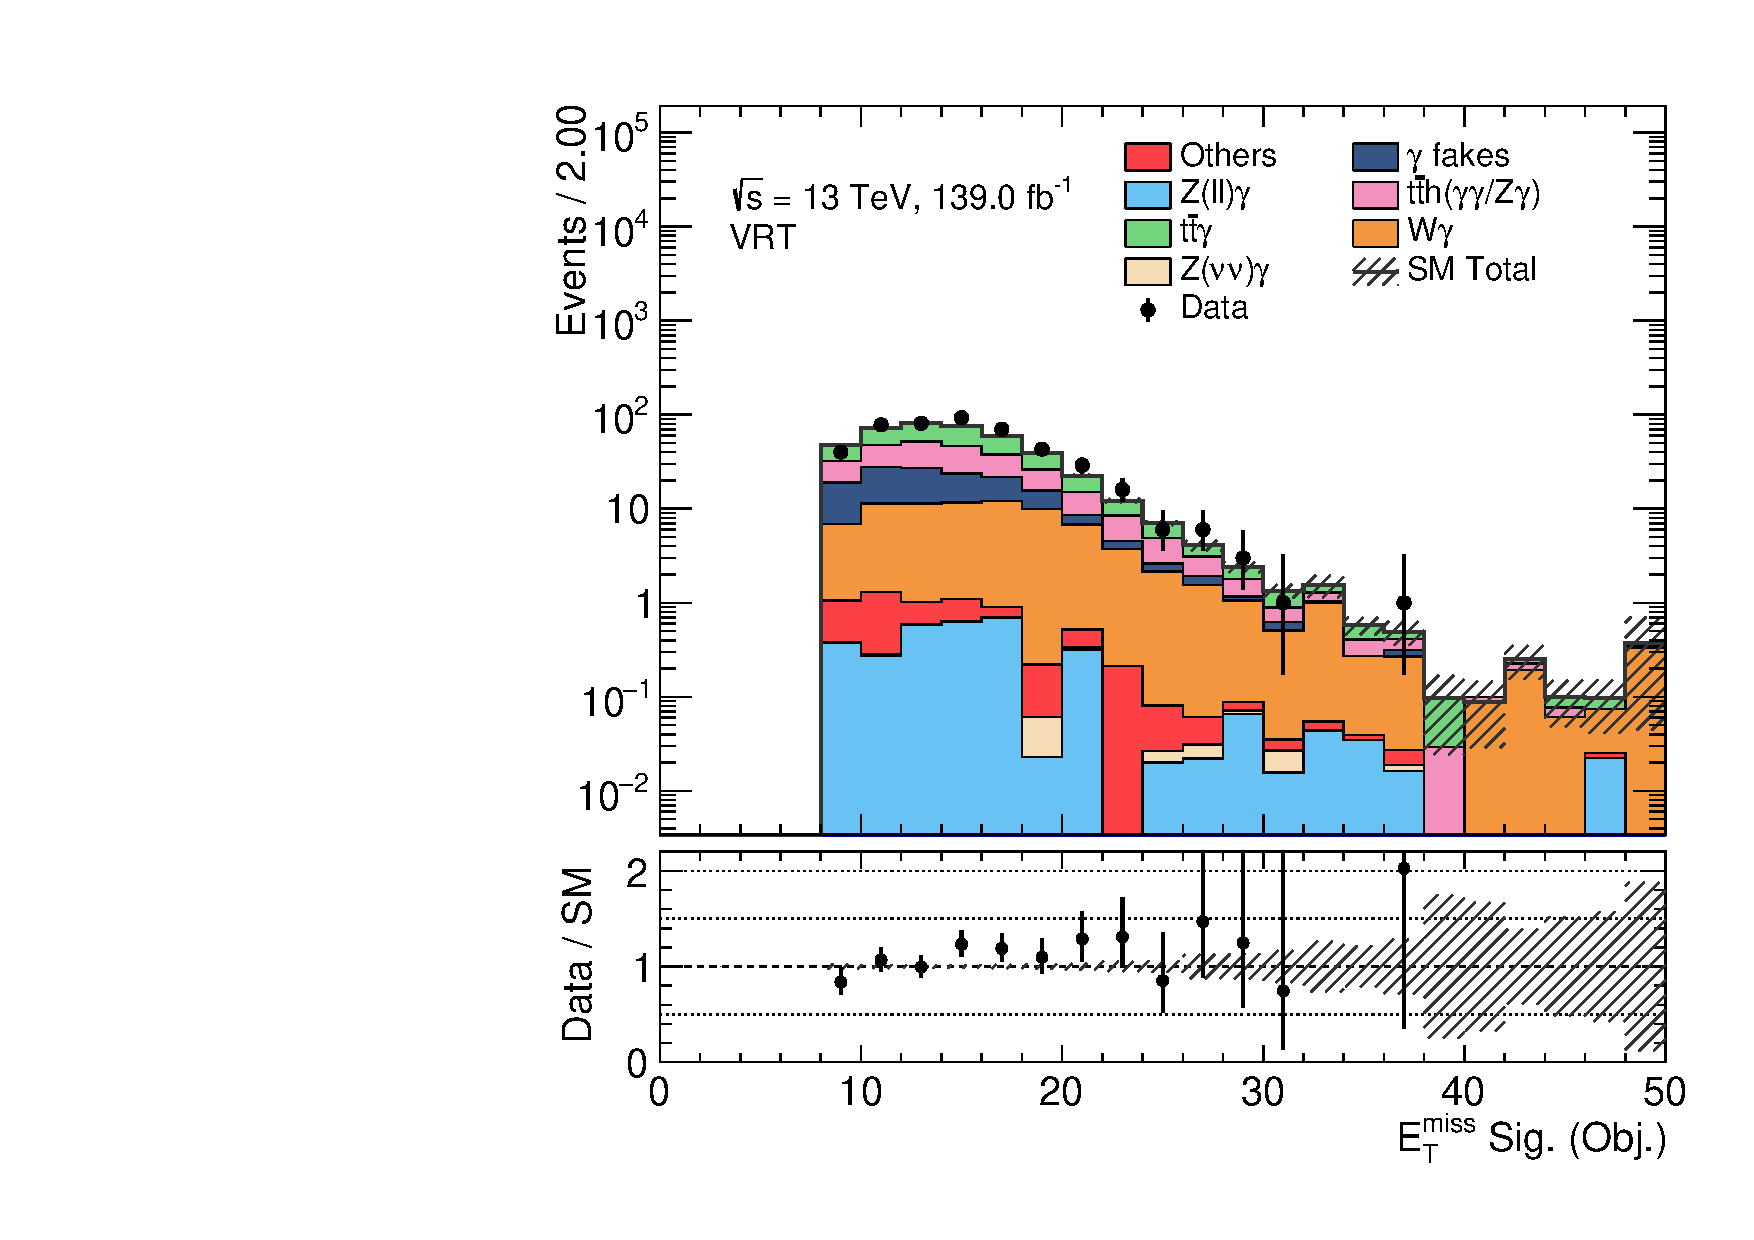
\includegraphics[width=0.24\textwidth]{images/analysis_EWK/v192_2_nosyst/can_VRT_met_sig_obj_afterFit.pdf}

    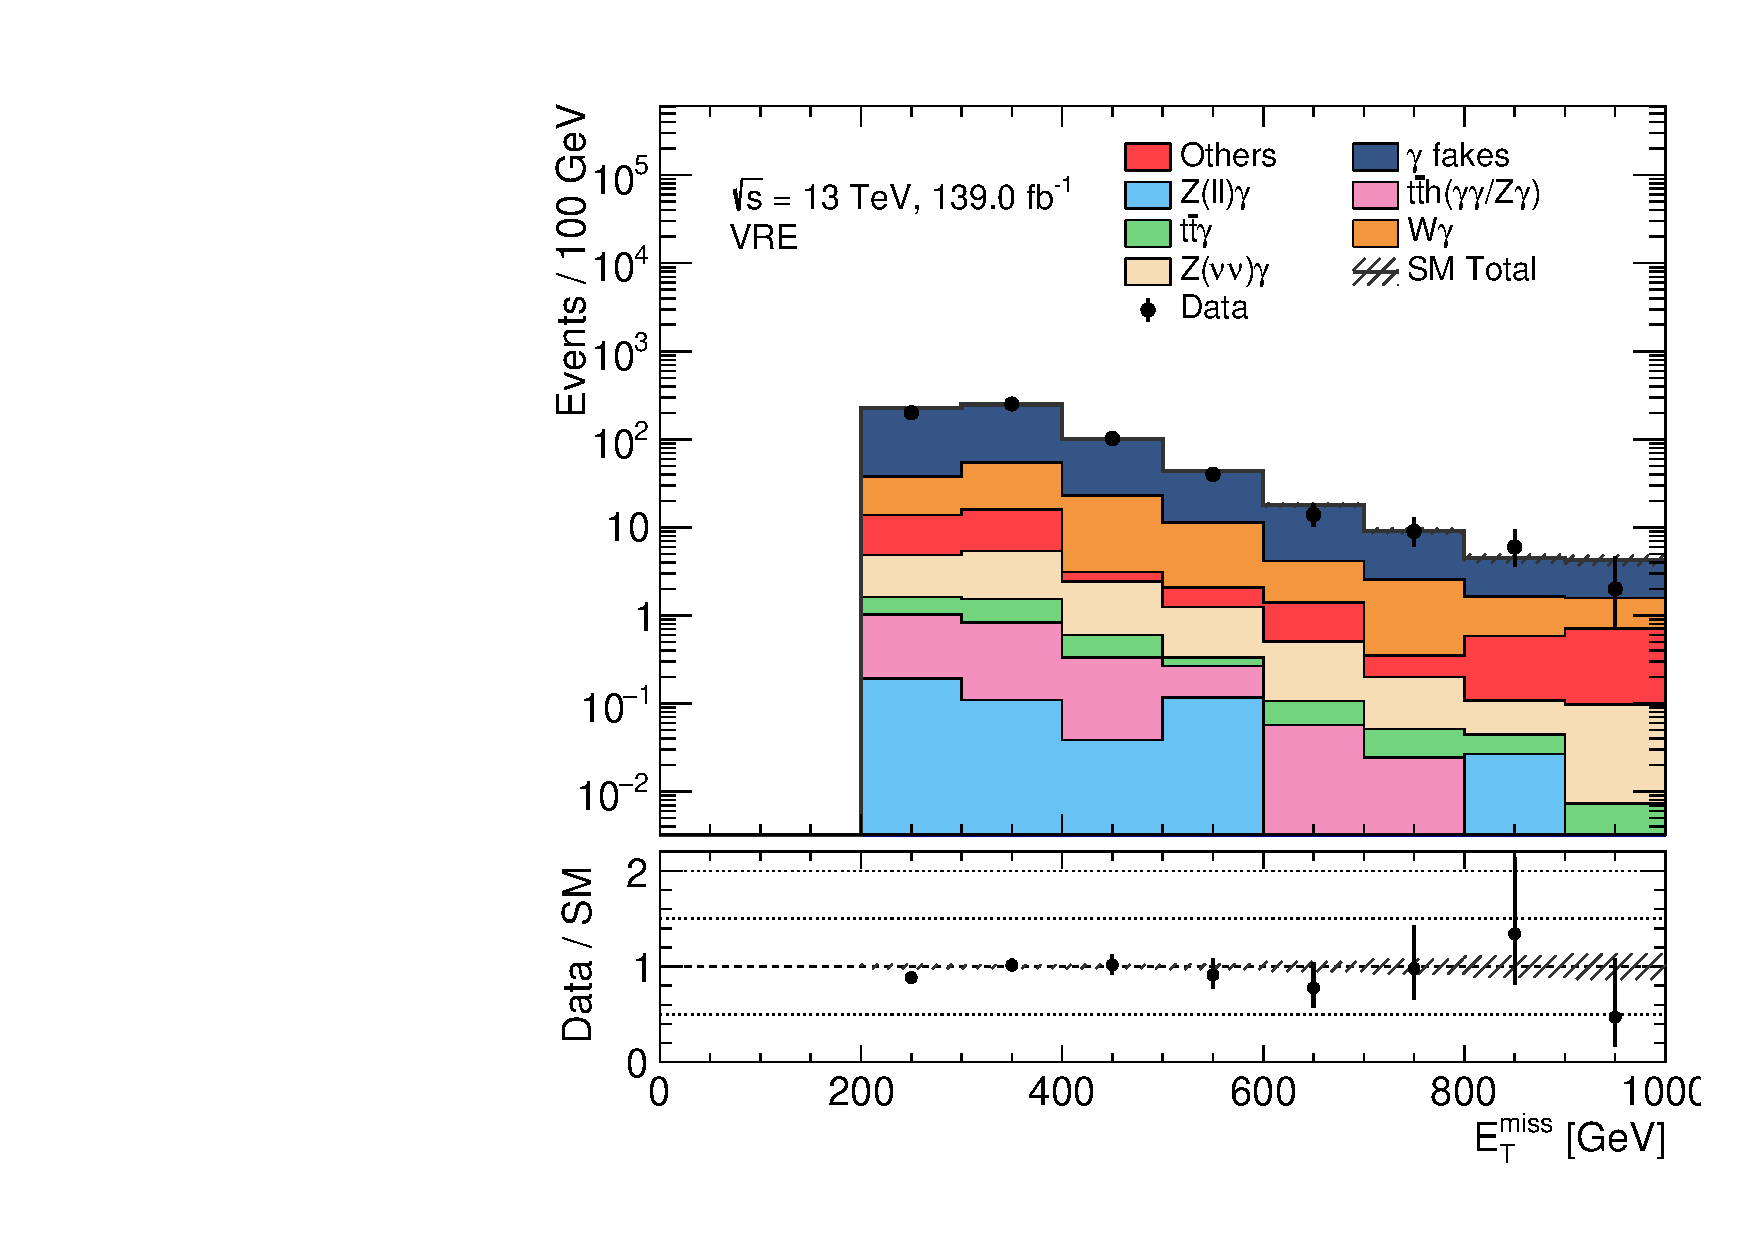
\includegraphics[width=0.24\textwidth]{images/analysis_EWK/v192_2_nosyst/can_VRE_met_et_afterFit.pdf}
    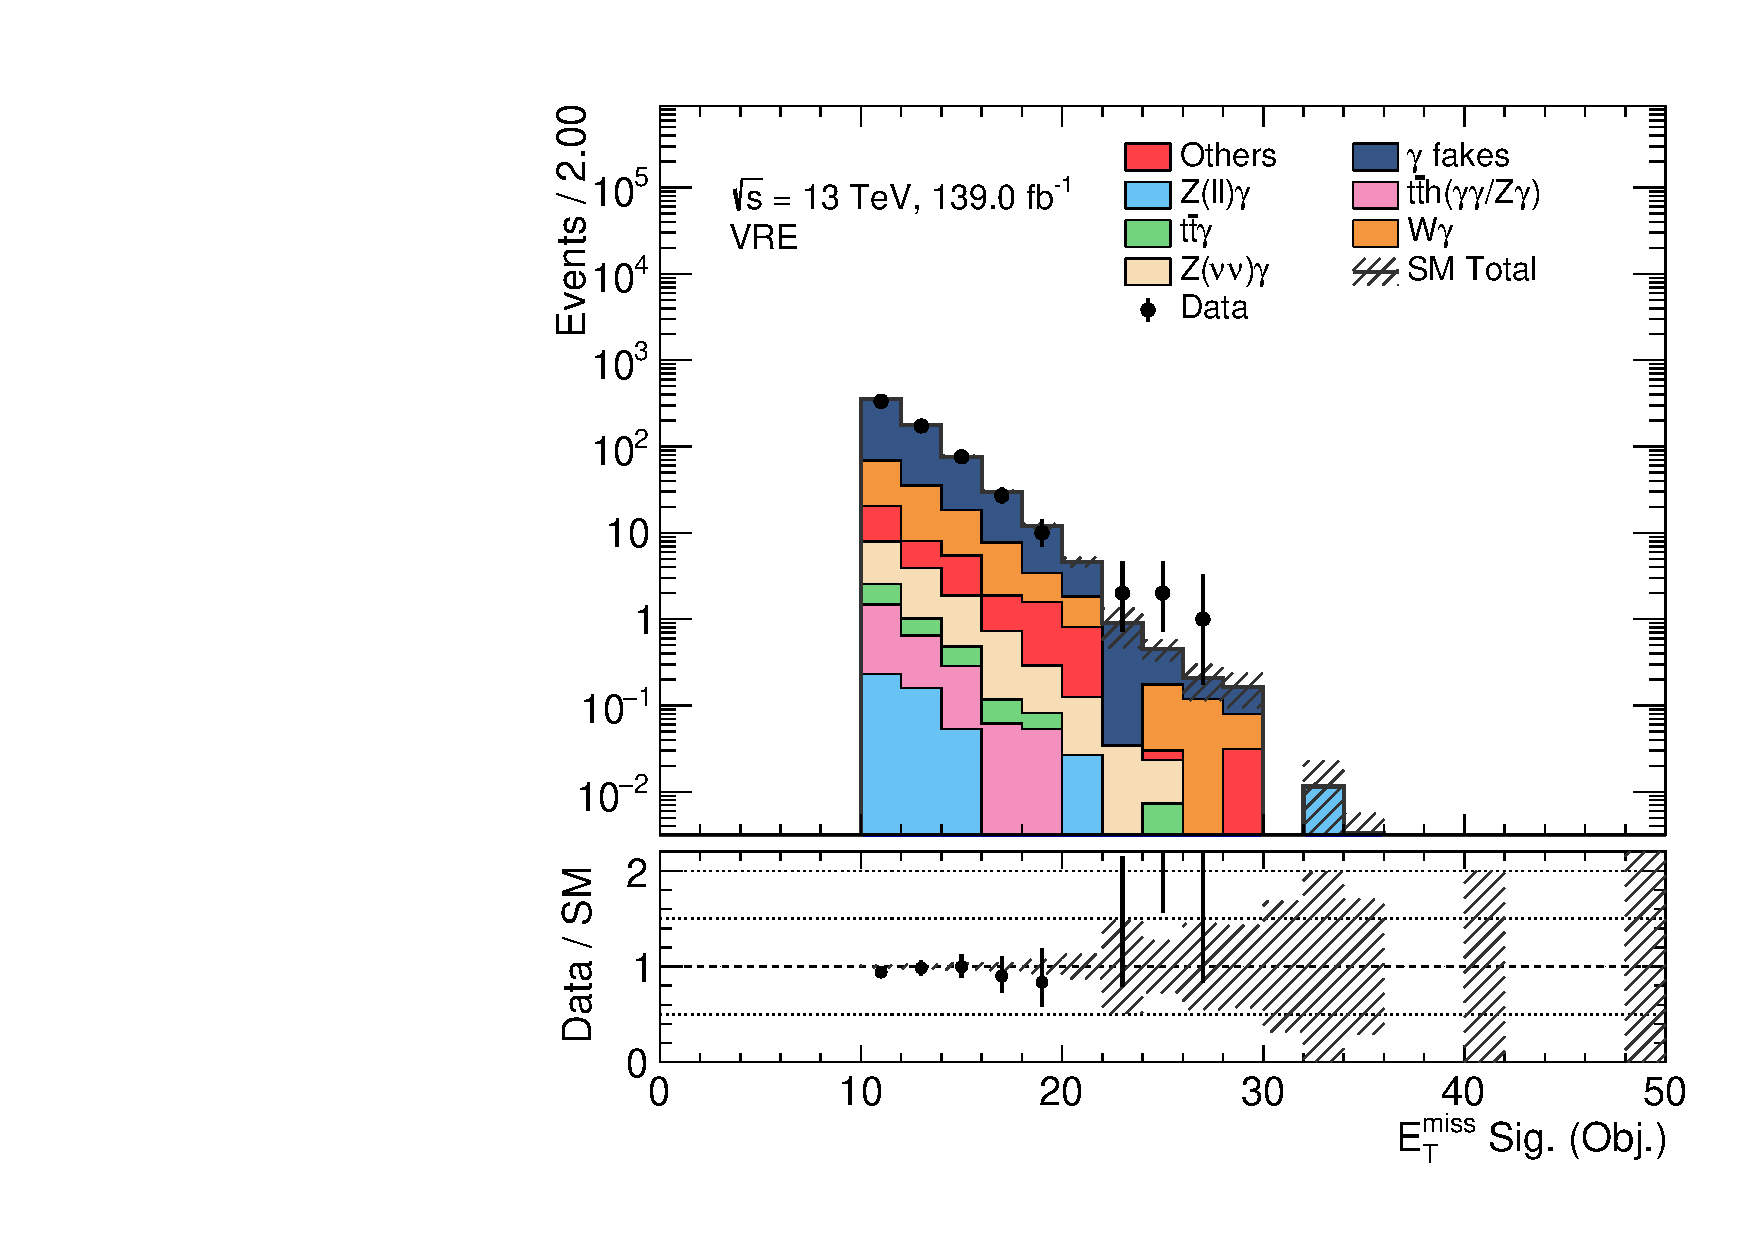
\includegraphics[width=0.24\textwidth]{images/analysis_EWK/v192_2_nosyst/can_VRE_met_sig_obj_afterFit.pdf}
    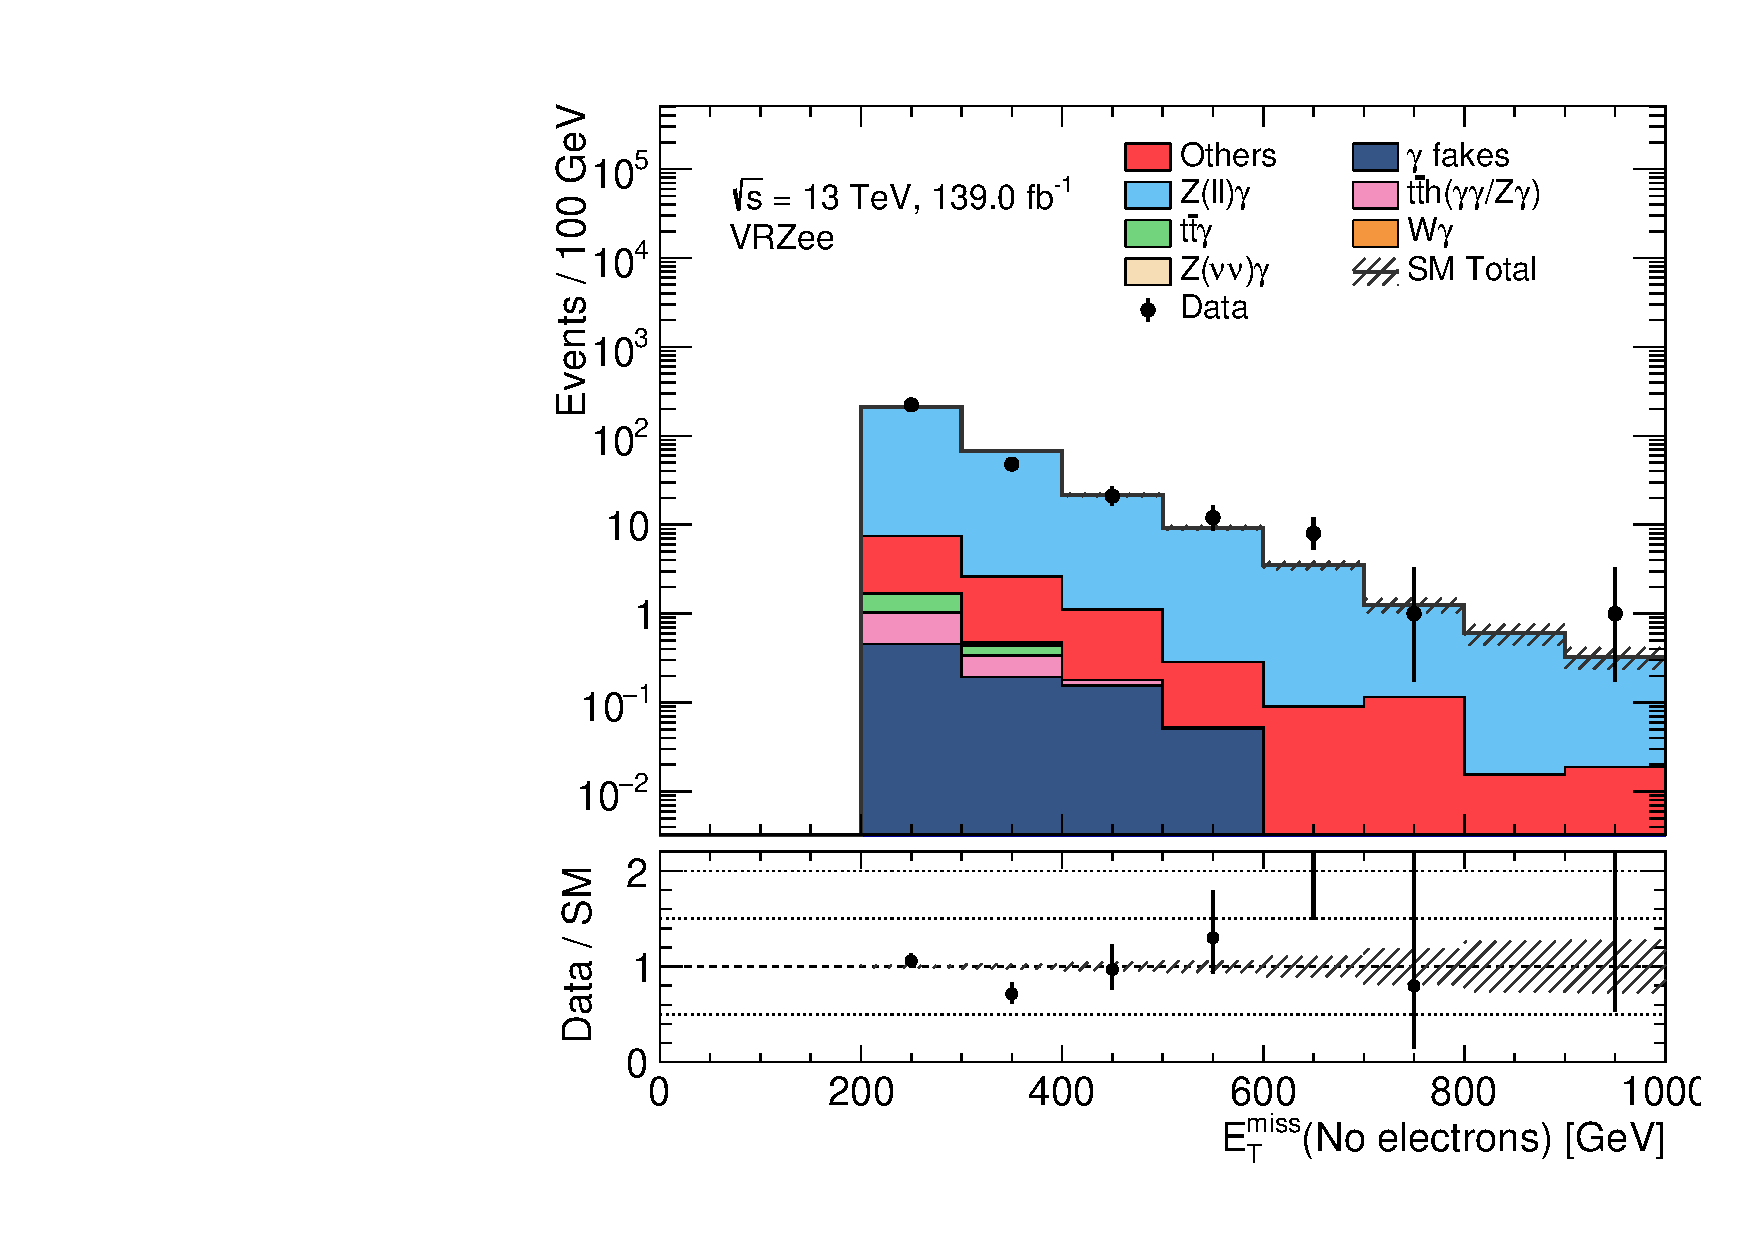
\includegraphics[width=0.24\textwidth]{images/analysis_EWK/v192_2_nosyst/can_VRZee_met_noele_et_afterFit.pdf}
    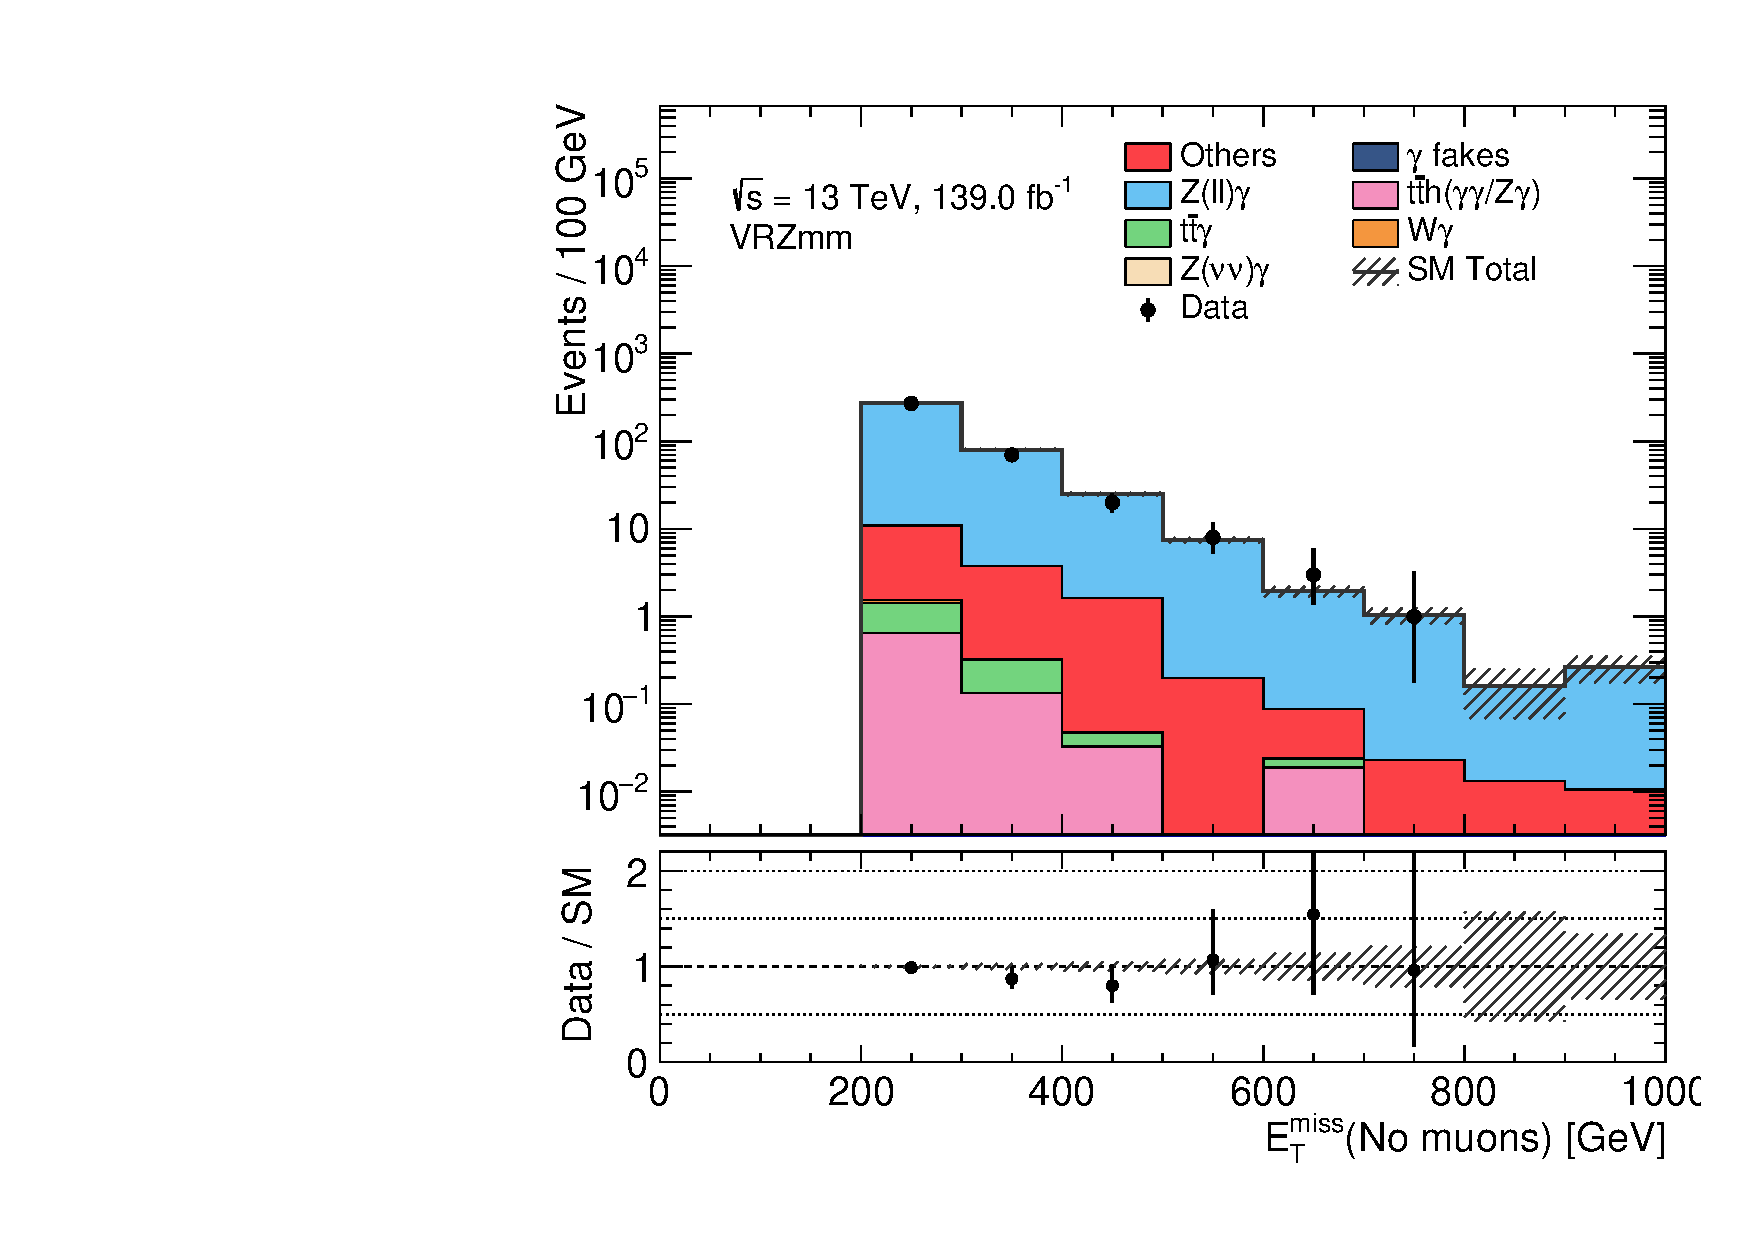
\includegraphics[width=0.24\textwidth]{images/analysis_EWK/v192_2_nosyst/can_VRZmm_met_nomuon_et_afterFit.pdf}

    \caption{Distribuciones preliminares de \met y $\mathcal{S}$ en las regiones de validación VRW, VRT y VRE, luego del ajuste de solo fondo para el análisis de producción electrodébil. Se muestra a su vez las distribuciones preliminares de \met en las VRZee y VRZmm removiendo los respectivos leptones en el cálculo de dicha variable. Las incertezas mostradas son sólo estadísticas. P}
    \label{fig:vr_ewk}

\end{figure}

En la Tabla \ref{tab:fit_result_sr} se muestran los resultados blinded en las regiones de señal de descubrimiento para el presente análisis. En la Figura \ref{fig:srd_ewk} se observan distribuciones para las regiones de señal de descubrimiento. Se puede apreciar como cada región de señal es sensible a un cierto rango de masas de \ninoone, llegándose a ser sensible hasta masas de \magn{750}{GeV}. Cabe mencionar, que al observar la distribución de $\mathcal{S}$, se puede apreciar que con cortes más estrictos de dicha variable, se obtienen valores de significancia más altos. Esto tiene como consecuencia una reducción importante del fondo, lo que conlleva a diversos problemáticas, como no encontrarse en el régimen asintótico para la aproximación de los estadísticos de prueba, o inconvenientes al ajustar los sistemáticos para PLR. Se priorizó entonces tener un número de fondo significante, al costo de una reducción de sensibilidad.
La Figura \ref{fig:sre_ewk} se muestran los límites esperados empleando ambos conjuntos de regiones de señal, donde se puede observar que con las regiones de señal de exclusión los límites son mejores.
% \solved{También se hizo los limites con un shape fit, y dan un poco mejor, el tema es que hay que explicar que es un shape fit...} no se explicar ni se menciona
Dichos limites son del orden de \magn{1200}{GeV}, lo que podría significar un importante aporte a los límites impuestos en la actualidad a dichos procesos, los cuales se observan en la Figura \ref{fig:ewk_limits}.


\begin{table}[ht!]
  \centering
  \caption{Estimación preliminar de los fondos y de la señal en las distintas regiones de señal luego del ajuste de solo fondo para el análisis de producción electrodébil.}
  \resizebox{\textwidth}{!}{\begin{tabular}{lrrrr}
\hline
Signal Regions & SRd\_200 & SRd\_300 & SRd\_400 & SRd\_500 \\
\hline
Observed events & - & - & - & - \\
\hline
Expected SM events & $115.31 \pm 4.03$ & $68.37 \pm 1.74$ & $25.08 \pm 0.88$ & $10.18 \pm 0.57$ \\
\hline
$Z(\nu\nu)\gamma$ & $84.16 \pm 3.60$ & $51.26 \pm 1.62$ & $18.89 \pm 0.79$ & $7.79 \pm 0.48$ \\
$t\bar{t}\gamma$ & $0.05 \pm 0.01$ & $0.05 \pm 0.01$ & $0.03 \pm 0.00$ & $0.01 \pm 0.00$ \\
$t\bar{t}h(\gamma\gamma/Z\gamma)$ & $0.25 \pm 0.02$ & $0.18 \pm 0.01$ & $0.11 \pm 0.01$ & $0.02 \pm 0.00$ \\
$W\gamma$ & $12.06 \pm 0.57$ & $5.79 \pm 0.22$ & $1.80 \pm 0.08$ & $0.97 \pm 0.06$ \\
$Z(ll)\gamma$ & $0.40 \pm 0.02$ & $0.16 \pm 0.01$ & $0.01 \pm 0.00$ & $0.02_{-0.02}^{+0.00}$ \\
$\gamma\ \text{fakes}$ & $17.05 \pm 2.31$ & $8.14 \pm 1.30$ & $2.97 \pm 0.21$ & $0.84 \pm 0.09$ \\
Others & $1.35 \pm 0.05$ & $2.79 \pm 0.05$ & $1.26 \pm 0.04$ & $0.56 \pm 0.03$ \\
\hline
 &  &  &  &  \\
\hline
$\gamma+Z, m_{\tilde{\chi}_{1}^{0}} = 150 \text{GeV}$ & $ 40.57 \pm 7.68 (Z=0.83)$ & $ 16.12 \pm 5.02 (Z=0.49)$ & $ 2.99 \pm 2.12 (Z=0.12)$ & $ 0.00 \pm 0.00 (Z=0.00)$ \\
$\gamma+Z, m_{\tilde{\chi}_{1}^{0}} = 250 \text{GeV}$ & $\cellcolor{lightgreen} 185.18 \pm 6.60 (Z=3.50)$ & $ 39.06 \pm 3.16 (Z=1.34)$ & $ 8.24 \pm 1.52 (Z=0.65)$ & $ 1.88 \pm 0.80 (Z=0.20)$ \\
$\gamma+Z, m_{\tilde{\chi}_{1}^{0}} = 350 \text{GeV}$ & $\cellcolor{lightgreen} 210.15 \pm 3.90 (Z=3.87)$ & $\cellcolor{lightgreen} 131.28 \pm 3.11 (Z=3.94)$ & $ 21.31 \pm 1.27 (Z=1.78)$ & $ 3.56 \pm 0.53 (Z=0.55)$ \\
$\gamma+Z, m_{\tilde{\chi}_{1}^{0}} = 450 \text{GeV}$ & $ 125.96 \pm 3.61 (Z=2.53)$ & $\cellcolor{lightgreen} 106.62 \pm 3.33 (Z=3.34)$ & $\cellcolor{lightgreen} 50.31 \pm 2.31 (Z=3.74)$ & $ 10.51 \pm 1.07 (Z=1.77)$ \\
$\gamma+Z, m_{\tilde{\chi}_{1}^{0}} = 550 \text{GeV}$ & $ 73.50 \pm 2.76 (Z=1.54)$ & $ 69.51 \pm 2.69 (Z=2.32)$ & $\cellcolor{lightgreen} 52.35 \pm 2.35 (Z=3.86)$ & $\cellcolor{lightgreen} 24.79 \pm 1.63 (Z=3.73)$ \\
$\gamma+Z, m_{\tilde{\chi}_{1}^{0}} = 650 \text{GeV}$ & $ 36.42 \pm 1.74 (Z=0.73)$ & $ 35.51 \pm 1.72 (Z=1.22)$ & $ 30.67 \pm 1.61 (Z=2.47)$ & $\cellcolor{lightgreen} 21.94 \pm 1.35 (Z=3.38)$ \\
$\gamma+Z, m_{\tilde{\chi}_{1}^{0}} = 750 \text{GeV}$ & $ 18.52 \pm 1.02 (Z=0.29)$ & $ 18.25 \pm 1.01 (Z=0.58)$ & $ 16.72 \pm 0.97 (Z=1.40)$ & $ 13.90 \pm 0.88 (Z=2.29)$ \\
% $\gamma+Z, m_{\tilde{\chi}_{1}^{0}} = 850 \text{GeV}$ & $ 11.15 \pm 0.57 (Z=0.10)$ & $ 11.10 \pm 0.57 (Z=0.29)$ & $ 10.59 \pm 0.56 (Z=0.87)$ & $ 9.18 \pm 0.52 (Z=1.56)$ \\
\hline
$\gamma+h, m_{\tilde{\chi}_{1}^{0}} = 150 \text{GeV}$ & $ 12.34 \pm 4.15 (Z=0.13)$ & $ 2.41 \pm 1.72 (Z=0.00)$ & $ 0.00 \pm 0.00 (Z=0.00)$ & $ 0.00 \pm 0.00 (Z=0.00)$ \\
$\gamma+h, m_{\tilde{\chi}_{1}^{0}} = 250 \text{GeV}$ & $\cellcolor{lightgreen} 163.46 \pm 6.19 (Z=3.16)$ & $ 27.75 \pm 2.66 (Z=0.94)$ & $ 4.33 \pm 1.14 (Z=0.26)$ & $ 0.80 \pm 0.63 (Z=0.00)$ \\
$\gamma+h, m_{\tilde{\chi}_{1}^{0}} = 350 \text{GeV}$ & $\cellcolor{lightgreen} 197.81 \pm 3.79 (Z=3.69)$ & $\cellcolor{lightgreen} 121.60 \pm 2.99 (Z=3.71)$ & $ 17.52 \pm 1.15 (Z=1.47)$ & $ 2.60 \pm 0.45 (Z=0.35)$ \\
$\gamma+h, m_{\tilde{\chi}_{1}^{0}} = 450 \text{GeV}$ & $ 119.65 \pm 3.52 (Z=2.42)$ & $\cellcolor{lightgreen} 101.79 \pm 3.26 (Z=3.21)$ & $\cellcolor{lightgreen} 46.93 \pm 2.24 (Z=3.54)$ & $ 9.07 \pm 1.00 (Z=1.54)$ \\
$\gamma+h, m_{\tilde{\chi}_{1}^{0}} = 550 \text{GeV}$ & $ 70.84 \pm 2.70 (Z=1.49)$ & $ 67.56 \pm 2.64 (Z=2.26)$ & $\cellcolor{lightgreen} 50.70 \pm 2.30 (Z=3.76)$ & $\cellcolor{lightgreen} 23.19 \pm 1.57 (Z=3.54)$ \\
$\gamma+h, m_{\tilde{\chi}_{1}^{0}} = 650 \text{GeV}$ & $ 33.64 \pm 1.67 (Z=0.67)$ & $ 32.96 \pm 1.66 (Z=1.13)$ & $ 28.64 \pm 1.55 (Z=2.33)$ & $\cellcolor{lightgreen} 20.49 \pm 1.31 (Z=3.20)$ \\
$\gamma+h, m_{\tilde{\chi}_{1}^{0}} = 750 \text{GeV}$ & $ 17.63 \pm 1.00 (Z=0.27)$ & $ 17.51 \pm 0.99 (Z=0.55)$ & $ 16.45 \pm 0.96 (Z=1.38)$ & $ 13.98 \pm 0.89 (Z=2.31)$ \\
% $\gamma+h, m_{\tilde{\chi}_{1}^{0}} = 850 \text{GeV}$ & $ 10.76 \pm 0.56 (Z=0.09)$ & $ 10.73 \pm 0.56 (Z=0.27)$ & $ 10.30 \pm 0.55 (Z=0.84)$ & $ 9.01 \pm 0.52 (Z=1.53)$ \\
\hline
\end{tabular}
}
  \label{tab:fit_result_sr}
\end{table}


\begin{figure}[ht!]
  \centering

    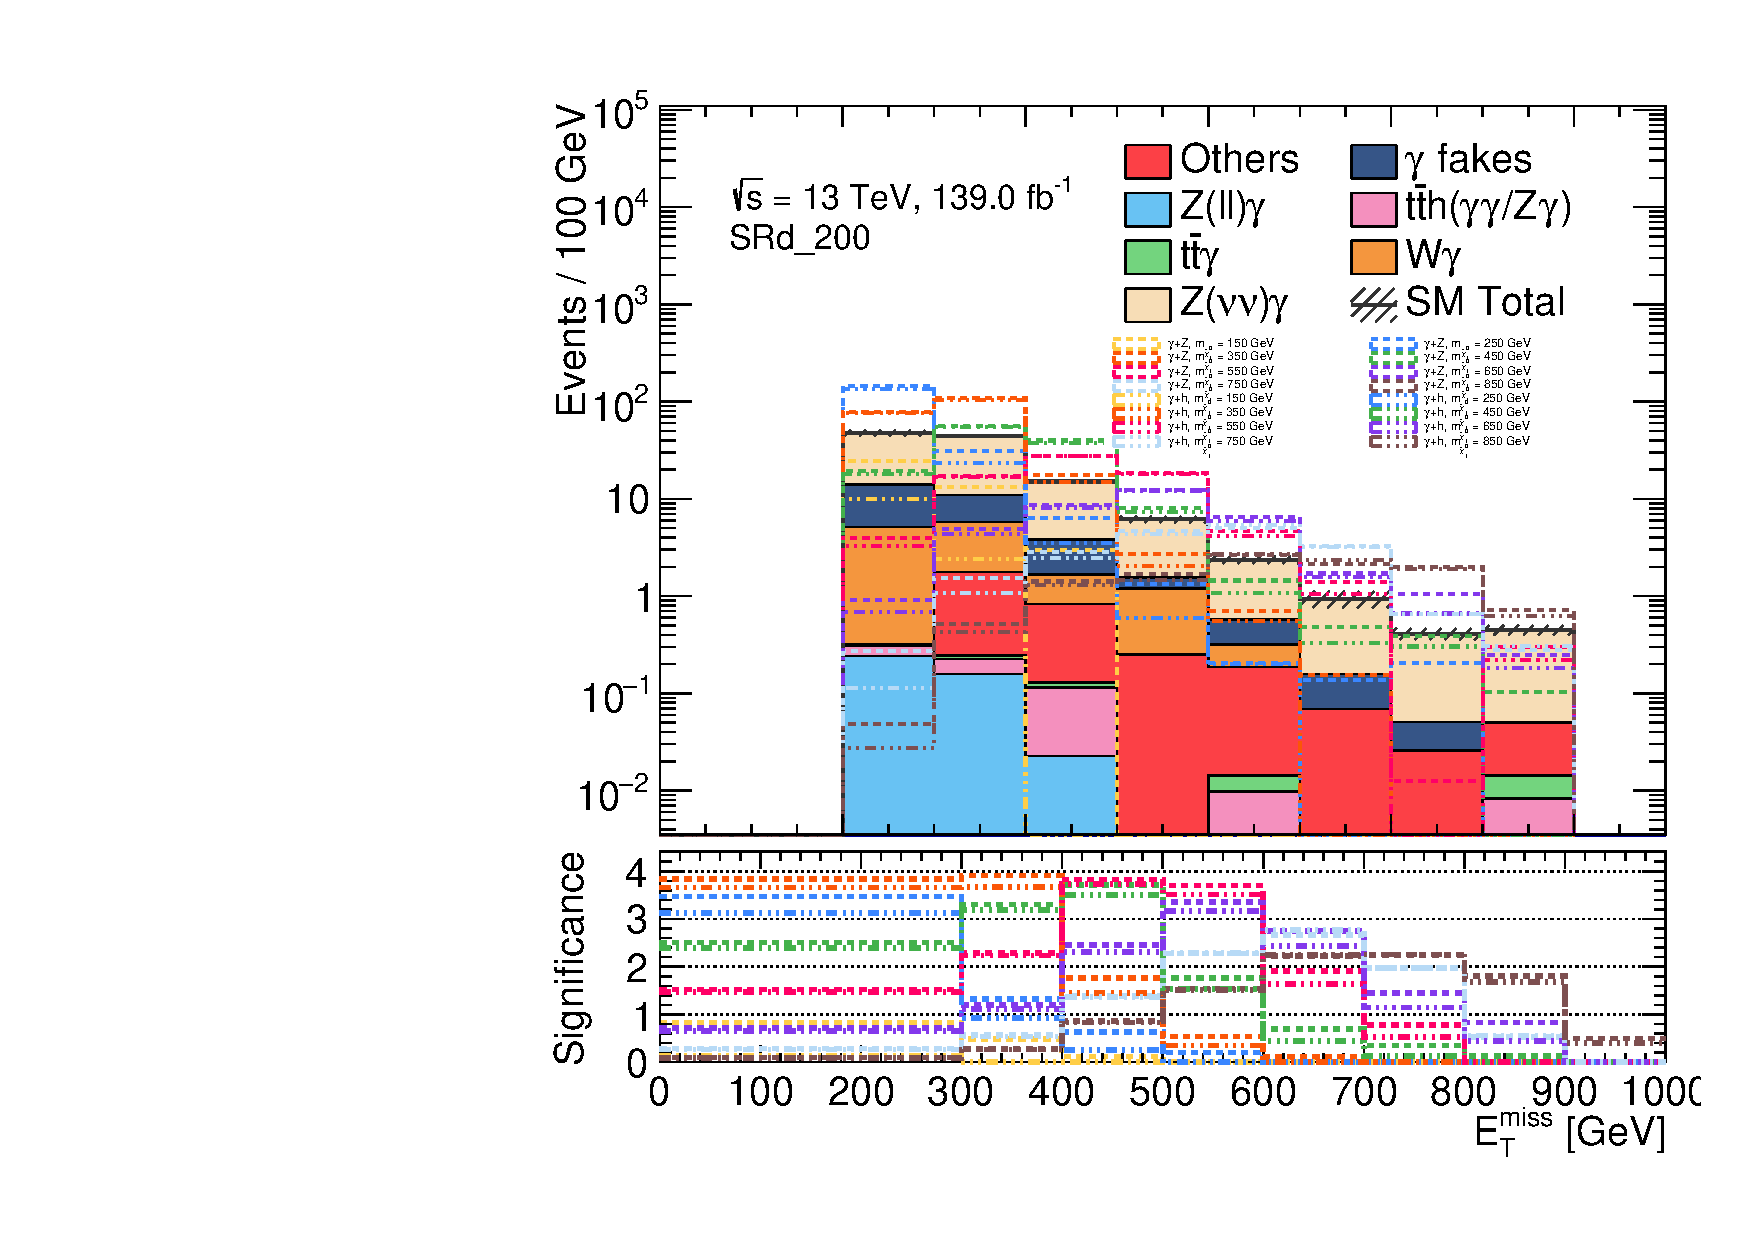
\includegraphics[width=0.49\textwidth]{images/analysis_EWK/v192_2_nosyst/can_SRd_200_met_et_afterFit.pdf}
    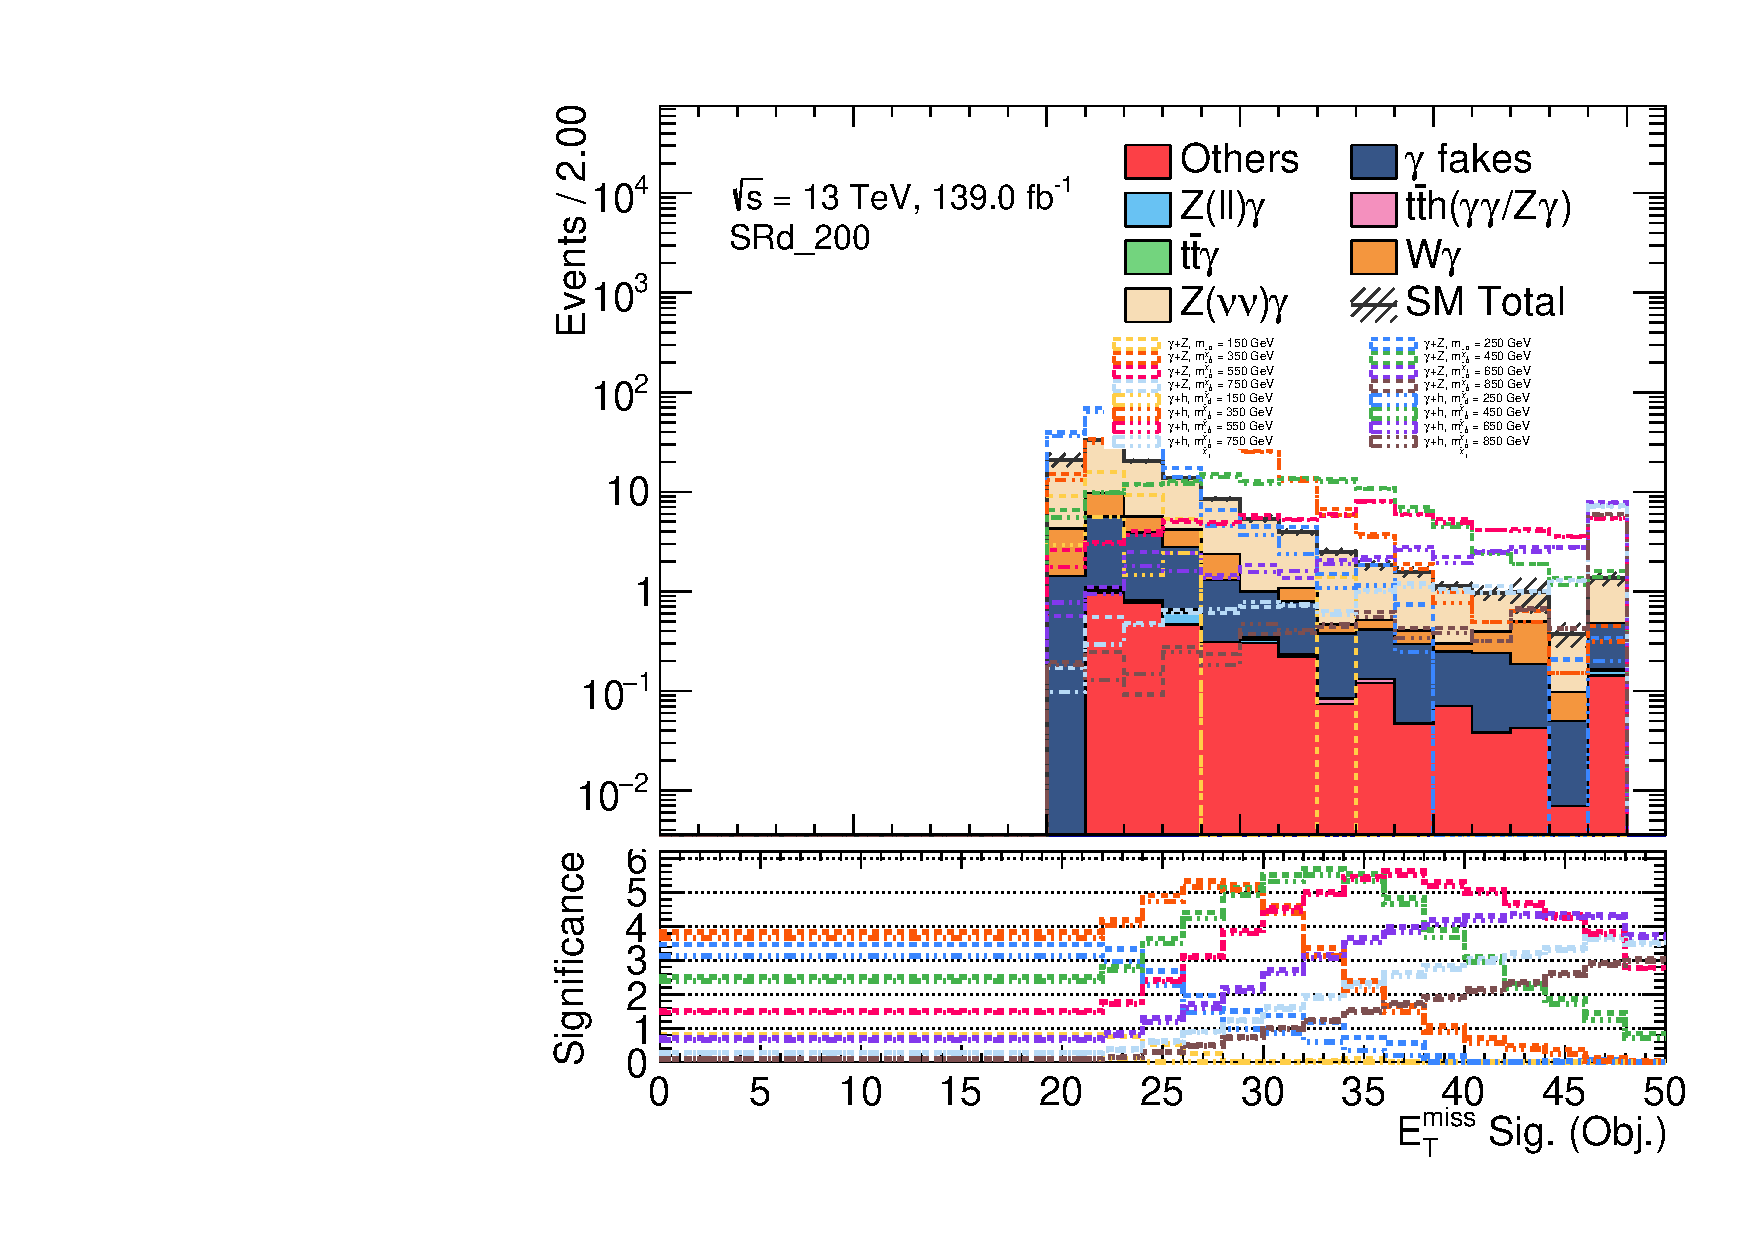
\includegraphics[width=0.49\textwidth]{images/analysis_EWK/v192_2_nosyst/can_SRd_200_met_sig_obj_afterFit.pdf}

    \caption{Distribuciones preliminares de \met y $\mathcal{S}$ en la región de señal SRd\_200 luego del ajuste de solo fondo, para el análisis de producción electrodébil. Las incertezas mostradas son sólo estadísticas.}
    \label{fig:srd_ewk}

\end{figure}

\begin{figure}[ht!]
  \centering

    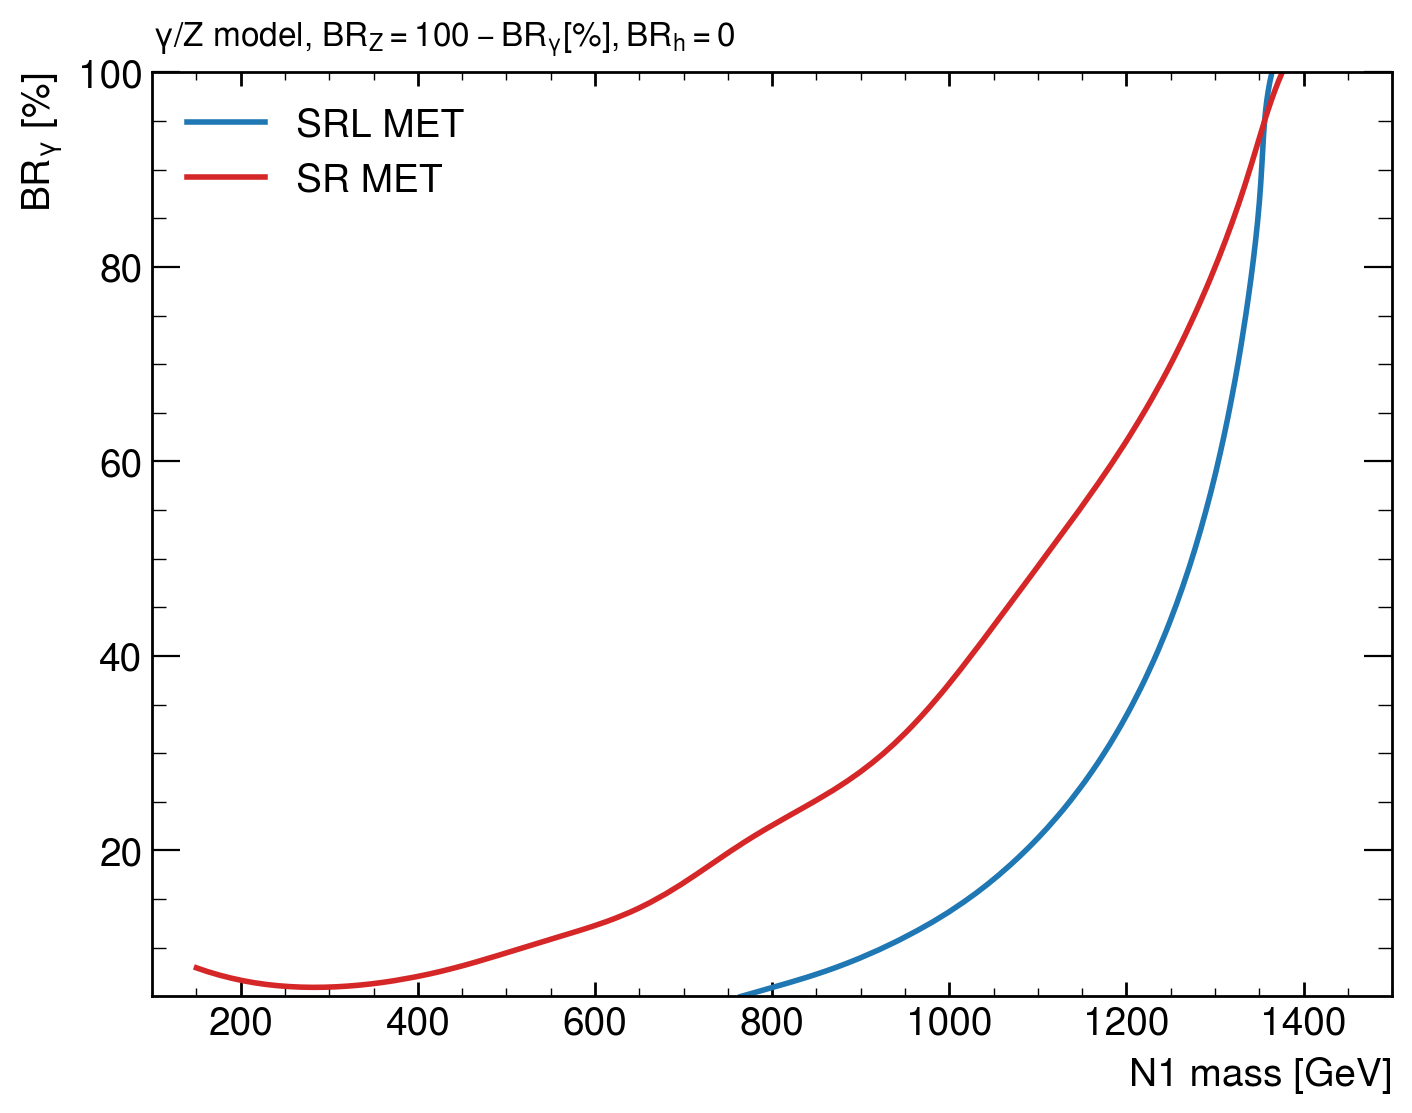
\includegraphics[width=0.49\textwidth]{images/analysis_EWK/plots_exp_excl_ewk/expected_limit_mass_vs_BR_yZ_cmp_SRL_vs_SR.png}
    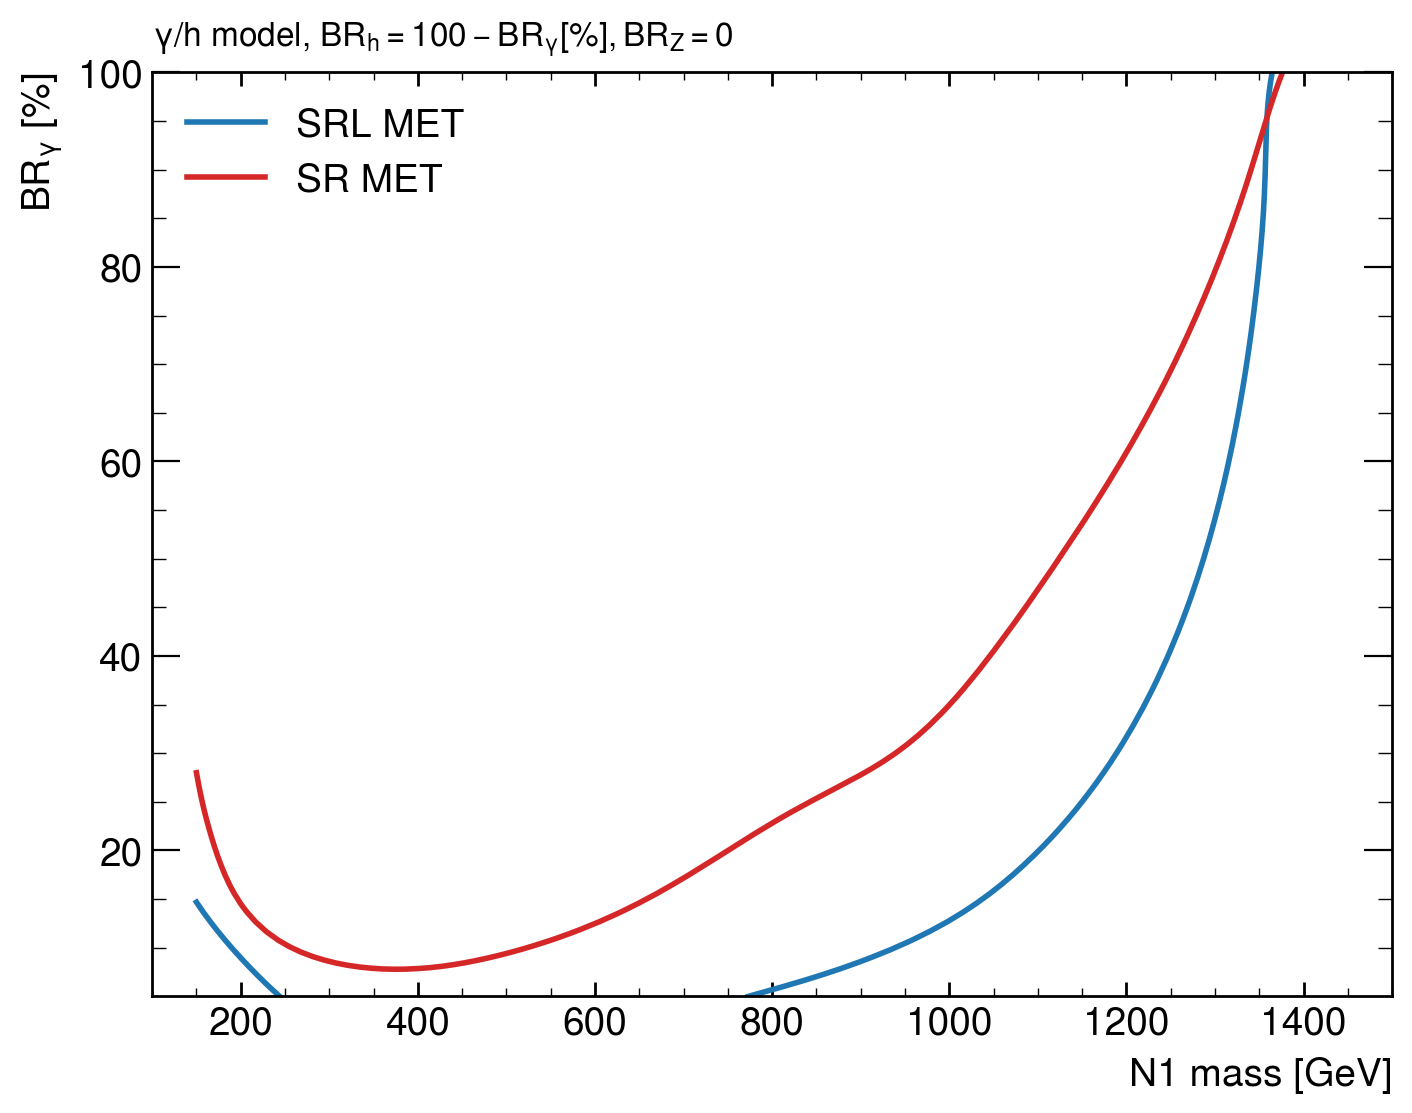
\includegraphics[width=0.49\textwidth]{images/analysis_EWK/plots_exp_excl_ewk/expected_limit_mass_vs_BR_yh_cmp_SRL_vs_SR.png}

    \caption{Límites esperados en función de la fracción de decaimiento del \ninoone a $\gamma+\gravino$ y su masa, para el modelo <<ph+Z>> (izquierda) y el modelo <<ph+h>>, comparando los resultados obtenidos empleando las regiones de señal de descubrimiento (rojo) y las de exclusión (azul).}
    \label{fig:sre_ewk}

\end{figure}

En la Figura \ref{fig:pull_ewk} se muestra el resumen de todos los fondos estimados y datos observados (excepto en las SRs) en todas las regiones del análisis.



\begin{figure}[ht!]
  \centering

    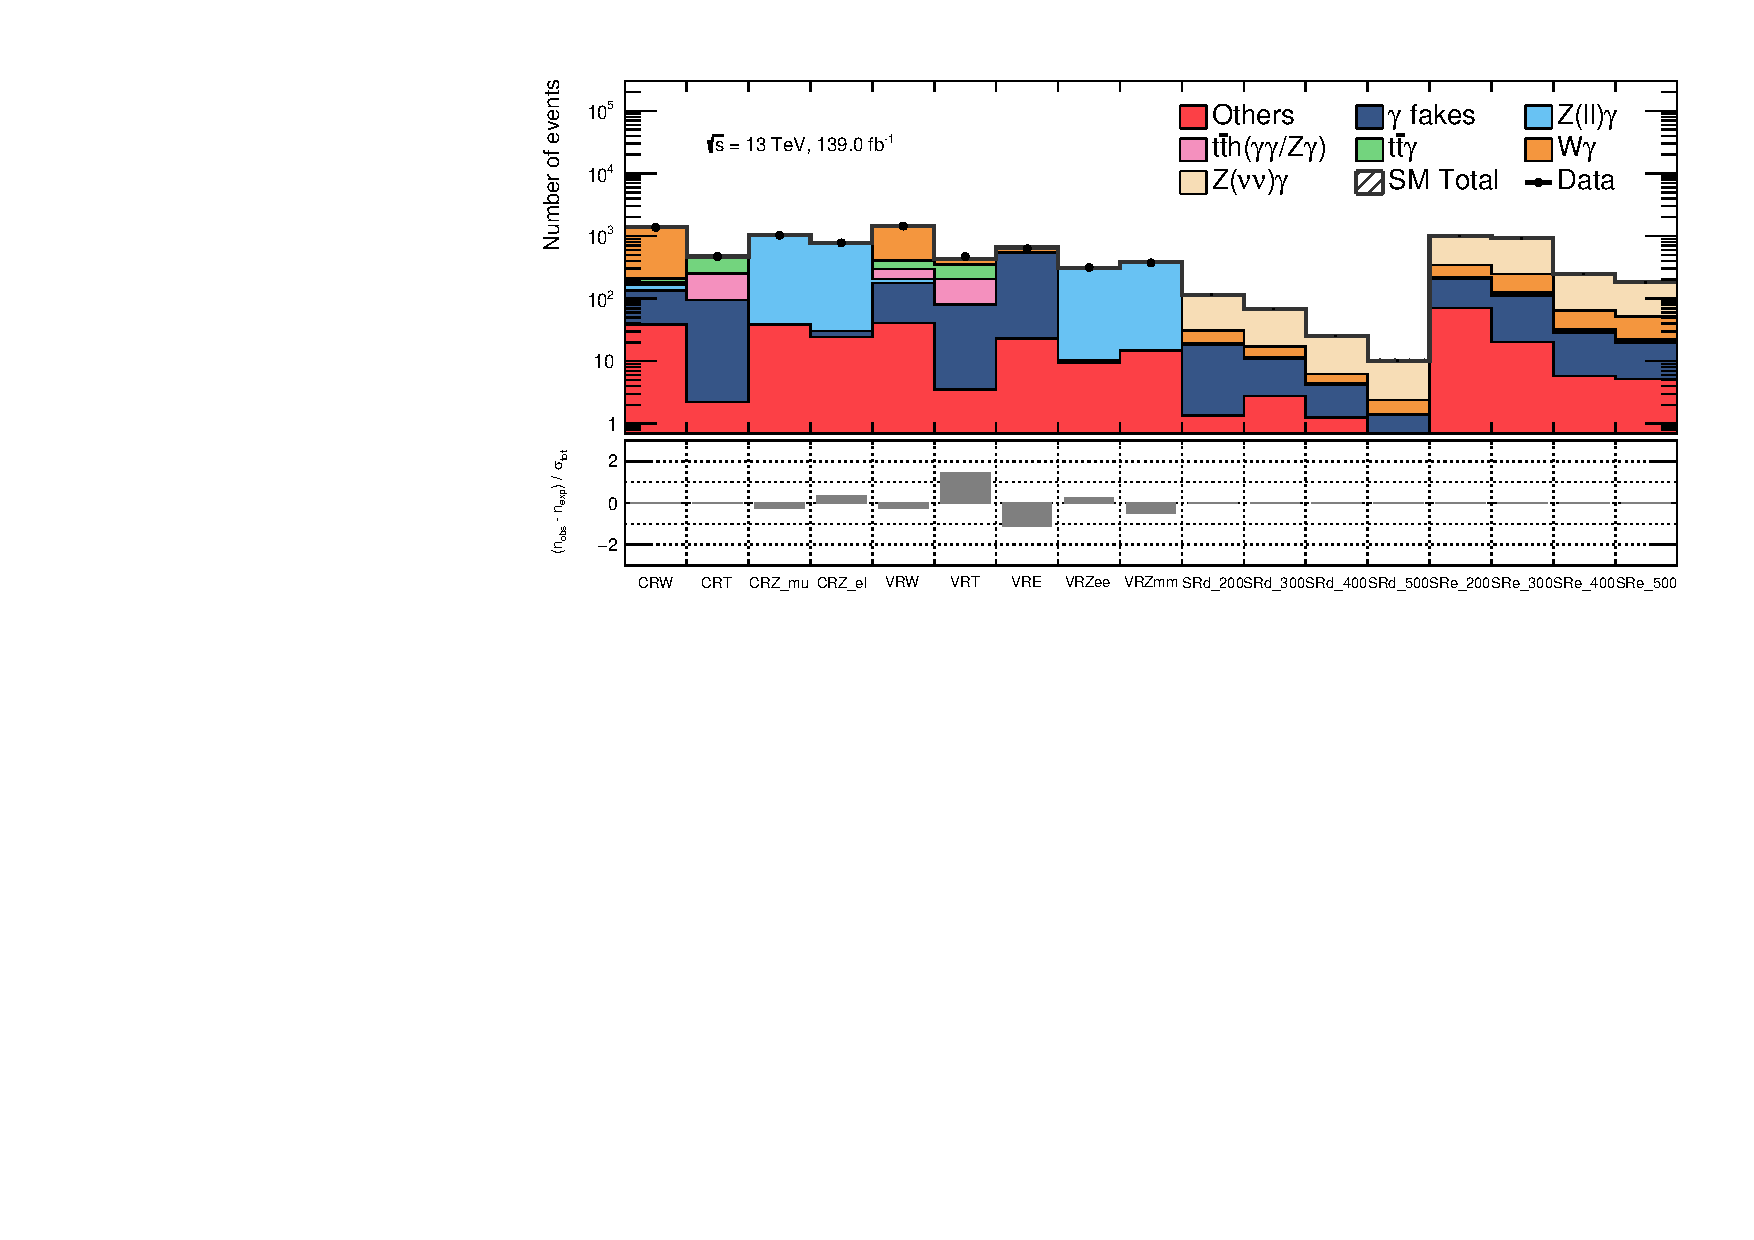
\includegraphics[width=\textwidth]{images/analysis_EWK/v192_2_nosyst/regions_pull.pdf}

    \caption{Resumen de las estimaciones de fondos y datos observados para las distintas regiones del análisis. Abajo se muestran las desviaciones entre los fondos y los datos.}
    \label{fig:pull_ewk}

\end{figure}

\begin{figure}[ht!]
  \centering

    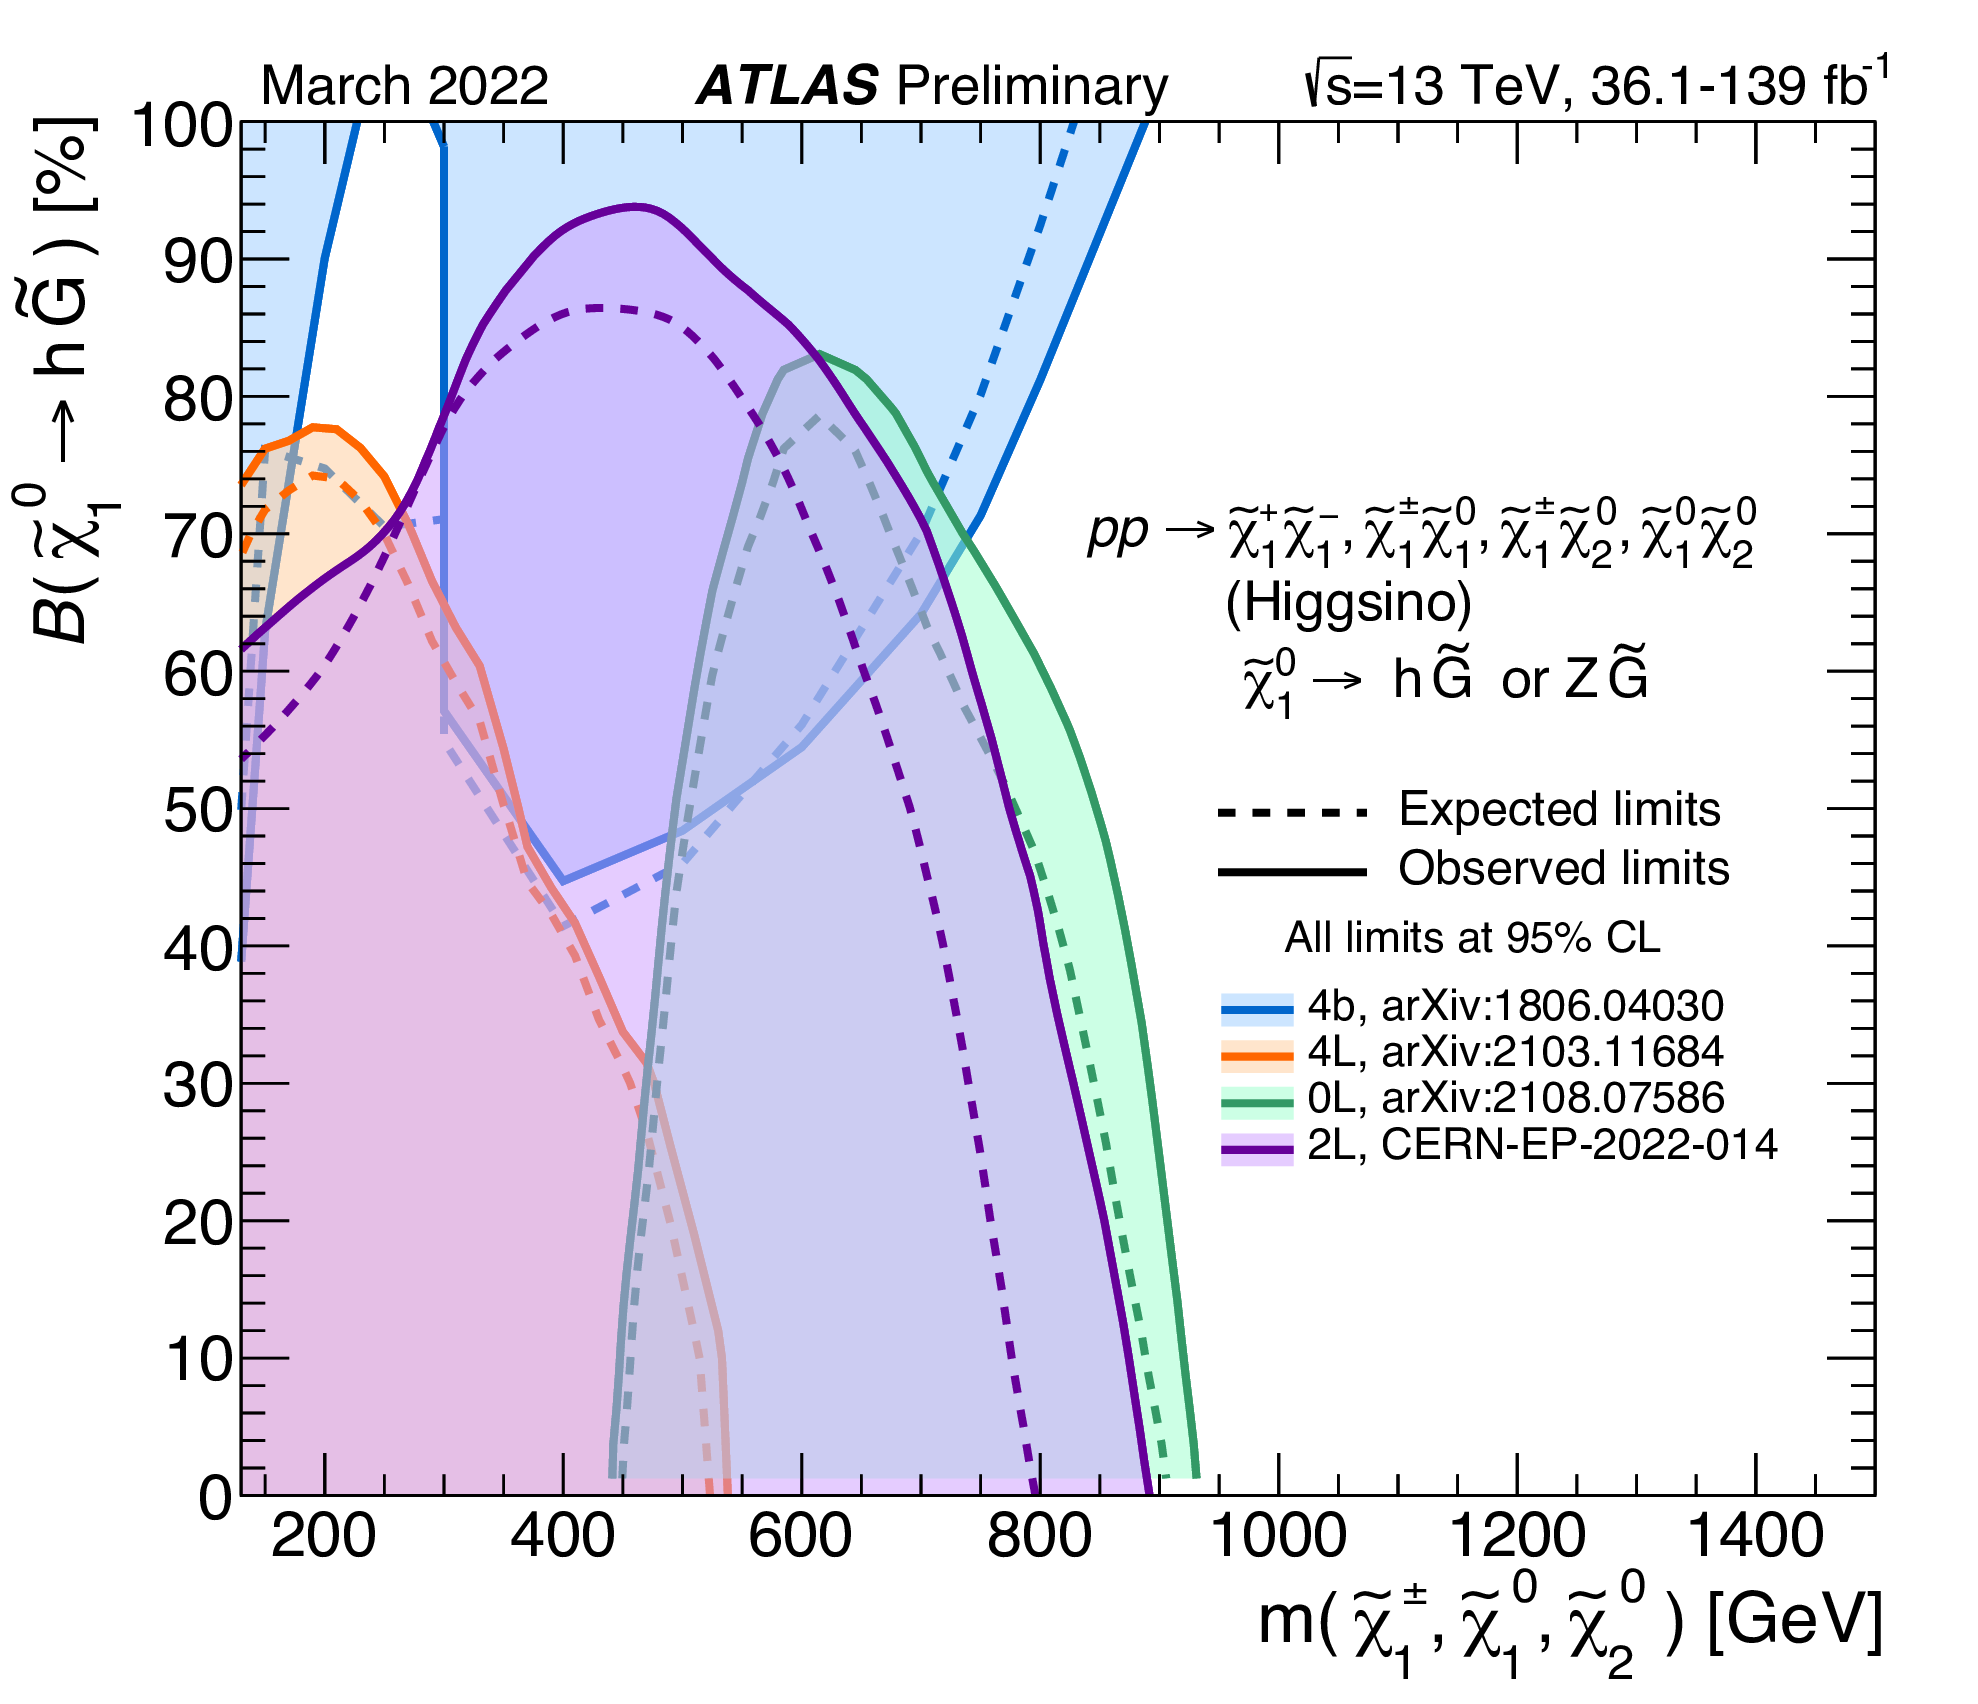
\includegraphics[width=0.65\textwidth]{images/analysis_EWK/actual_limits.png}

    \caption{Últimos límites impuestos a la masa de los gauginos para modelos GGM en función de su fracción de decaimiento a Higgs, combinando distintos resultados observados por la colaboración ATLAS \cite{susy_public_results}.}
    \label{fig:ewk_limits}

\end{figure}


